\documentclass[10pt,letterpaper]{article}
\usepackage[top=0.85in,left=2.00in,footskip=0.75in]{geometry}

% Use adjustwidth environment to exceed column width (see example table in text)
\usepackage{changepage}

% Use Unicode characters when possible
\usepackage[utf8]{inputenc}

% textcomp package and marvosym package for additional characters
\usepackage{textcomp,marvosym}

% fixltx2e package for \textsubscript
\usepackage{fixltx2e}

% amsmath and amssymb packages, useful for mathematical formulas and symbols
\usepackage{amsmath,amssymb}

% cite package, to clean up citations in the main text. Do not remove.
\usepackage{cite}

%lstlisting
\usepackage{listings}

% Use nameref to cite supporting information files (see Supporting Information section for more info)
\usepackage{nameref}
%\usepackage{hyperref}

% line numbers
\usepackage[right]{lineno}

% ligatures disabled
\usepackage{microtype}
%\DisableLigatures[f]{encoding = *, family = * }

% rotating package for sideways tables
\usepackage{rotating}

% Remove comment for double spacing
%\usepackage{setspace} 
%\doublespacing

%subfigures
\usepackage[lofdepth,lotdepth]{subfig}
% Text layout
%\raggedright
\setlength{\parindent}{0.5cm}
\textwidth 5.25in 
\textheight 8.75in

% Bold the 'Figure #' in the caption and separate it from the title/caption with a period
% Captions will be left justified
\usepackage[aboveskip=1pt,labelfont=bf,labelsep=period,justification=raggedright,singlelinecheck=off]{caption}
%\usepackage[aboveskip=1pt,labelfont=bf,labelsep=period,singlelinecheck=off]{caption}

% Use the PLoS provided BiBTeX style
\bibliographystyle{plos2009}

% Remove brackets from numbering in List of References
\makeatletter
\renewcommand{\@biblabel}[1]{\quad#1.}
\makeatother

% Leave date blank
\date{15.03.16}

% Header and Footer with logo
%\usepackage{lastpage,fancyhdr,graphicx}
%\pagestyle{myheadings}
%\pagestyle{fancy}
%\fancyhf{}
%\lhead{\includegraphics[natwidth=1.3in,natheight=0.4in]{PLOSlogo.png}}
%\rfoot{\thepage/\pageref{LastPage}}
%\renewcommand{\footrule}{\hrule height 2pt \vspace{2mm}}
%\fancyheadoffset[L]{2.25in}
%\fancyfootoffset[L]{2.25in}
%\lfoot{\sf PLOS}

%% Include all macros below

%\newcommand{\lorem}{{\bf LOREM}}
%\newcommand{\ipsum}{{\bf IPSUM}}

%% END MACROS SECTION


\begin{document}
\vspace*{0.30in}

% Title must be 150 characters or less
\begin{flushleft}
{\Large
\textbf\newline{ {\LARGE \textbf{Tecnologie Digitali - Relazione di Laboratorio: Misuratori di lunghezze d'onda}}}
}
\newline
% Insert Author names, affiliations and corresponding author email.
\\
Salvatore Bottaro\textsuperscript{1,*}
Lorenzo Maria Perrone\textsuperscript{1, $\dagger$},
%Name2 Surname\textsuperscript{2,\textpilcrow},
%Name3 Surname\textsuperscript{2,\textcurrency a},
%Name4 Surname\textsuperscript{2,\ddag},
%Name5 Surname\textsuperscript{2,\ddag},
%Name6 Surname\textsuperscript{2,\Yinyang},
%Name7 Surname\textsuperscript{3,*,\Yinyang}
\\
\bf{1} Dipartimento di Fisica, Università di Pisa
\\
%\bf{2} Affiliation Dept/Program/Center, Institution Name, City, State, Country
%\\
%\bf{3} Affiliation Dept/Program/Center, Institution Name, City, State, Country
%\\

% Insert additional author notes using the symbols described below. Insert symbol callouts after author names as necessary.
% 
% Remove or comment out the author notes below if they aren't used.
%
% Primary Equal Contribution Note
%\Yinyang These authors contributed equally to this work.

% Additional Equal Contribution Note
%\ddag These authors also contributed equally to this work.

% Current address notes
%\textcurrency a Insert current address of first author with an address update
% \textcurrency b Insert current address of second author with an address update
% \textcurrency c Insert current address of third author with an address update

% Deceased author note
%\dag Deceased

% Group/Consortium Author Note
%\textpilcrow Insert Collaborative Author line here
* E-mail: salvo.bottaro\\
$\dagger$ E-mail: lorenzo.perrone.lmp@gmail.com
\end{flushleft}

\section{Misuratore analogico di lunghezza d'onda}
Come seconda parte dell'esperienza, ci è stato messo a disposizione un integrato analogico, il \textsc{ws-7.56-to5} prodotto dalla Pacific Silicon Sensor, composto da due giunzioni p-n costruite sullo stesso substrato, come visibile nello schema in Figura (\ref{fig:schema_analog_sensor}). I due fotodiodi possiedono curve di responsività alla radiazione incidente differenti (il principio di funzionamento è lo stesso del sensore digitale \textsc{apds-9301}): il diodo superiore ha una risposta maggiore al blu, il secondo, quello inferiore, ha il picco sul rosso. Viene garantito che il rapporto dei due segnali è indipendente dalla luminosità incidente, purchè si sia in condizione di non saturazione; per tale motivo è possibile utilizzare la quantità $log(CH1/CH2)$ per stabilire una corrispondenza biunivoca con la lunghezza d'onda del segnale incidente. La curva di calibrazione per il nostro sensore è riportata in Figura (\ref{fig:calibrazione_analog}).\\

\begin{figure}
\centering
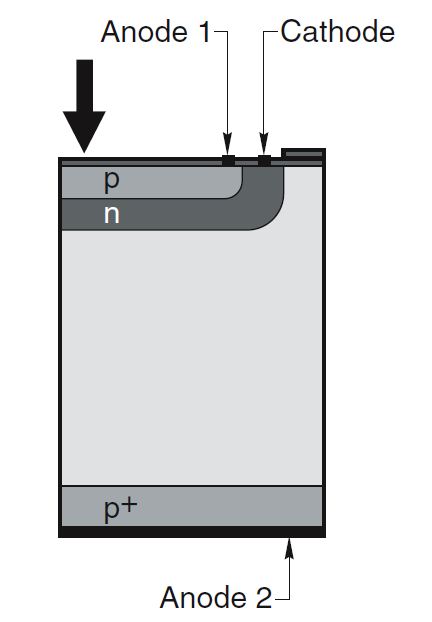
\includegraphics[width=0.2\linewidth]{./schema_analog_sensor}
\caption{Schema costruttivo dei fotodiodi del WS-765-TO5.}
\label{fig:schema_analog_sensor}
\end{figure}

\begin{figure}
\centering
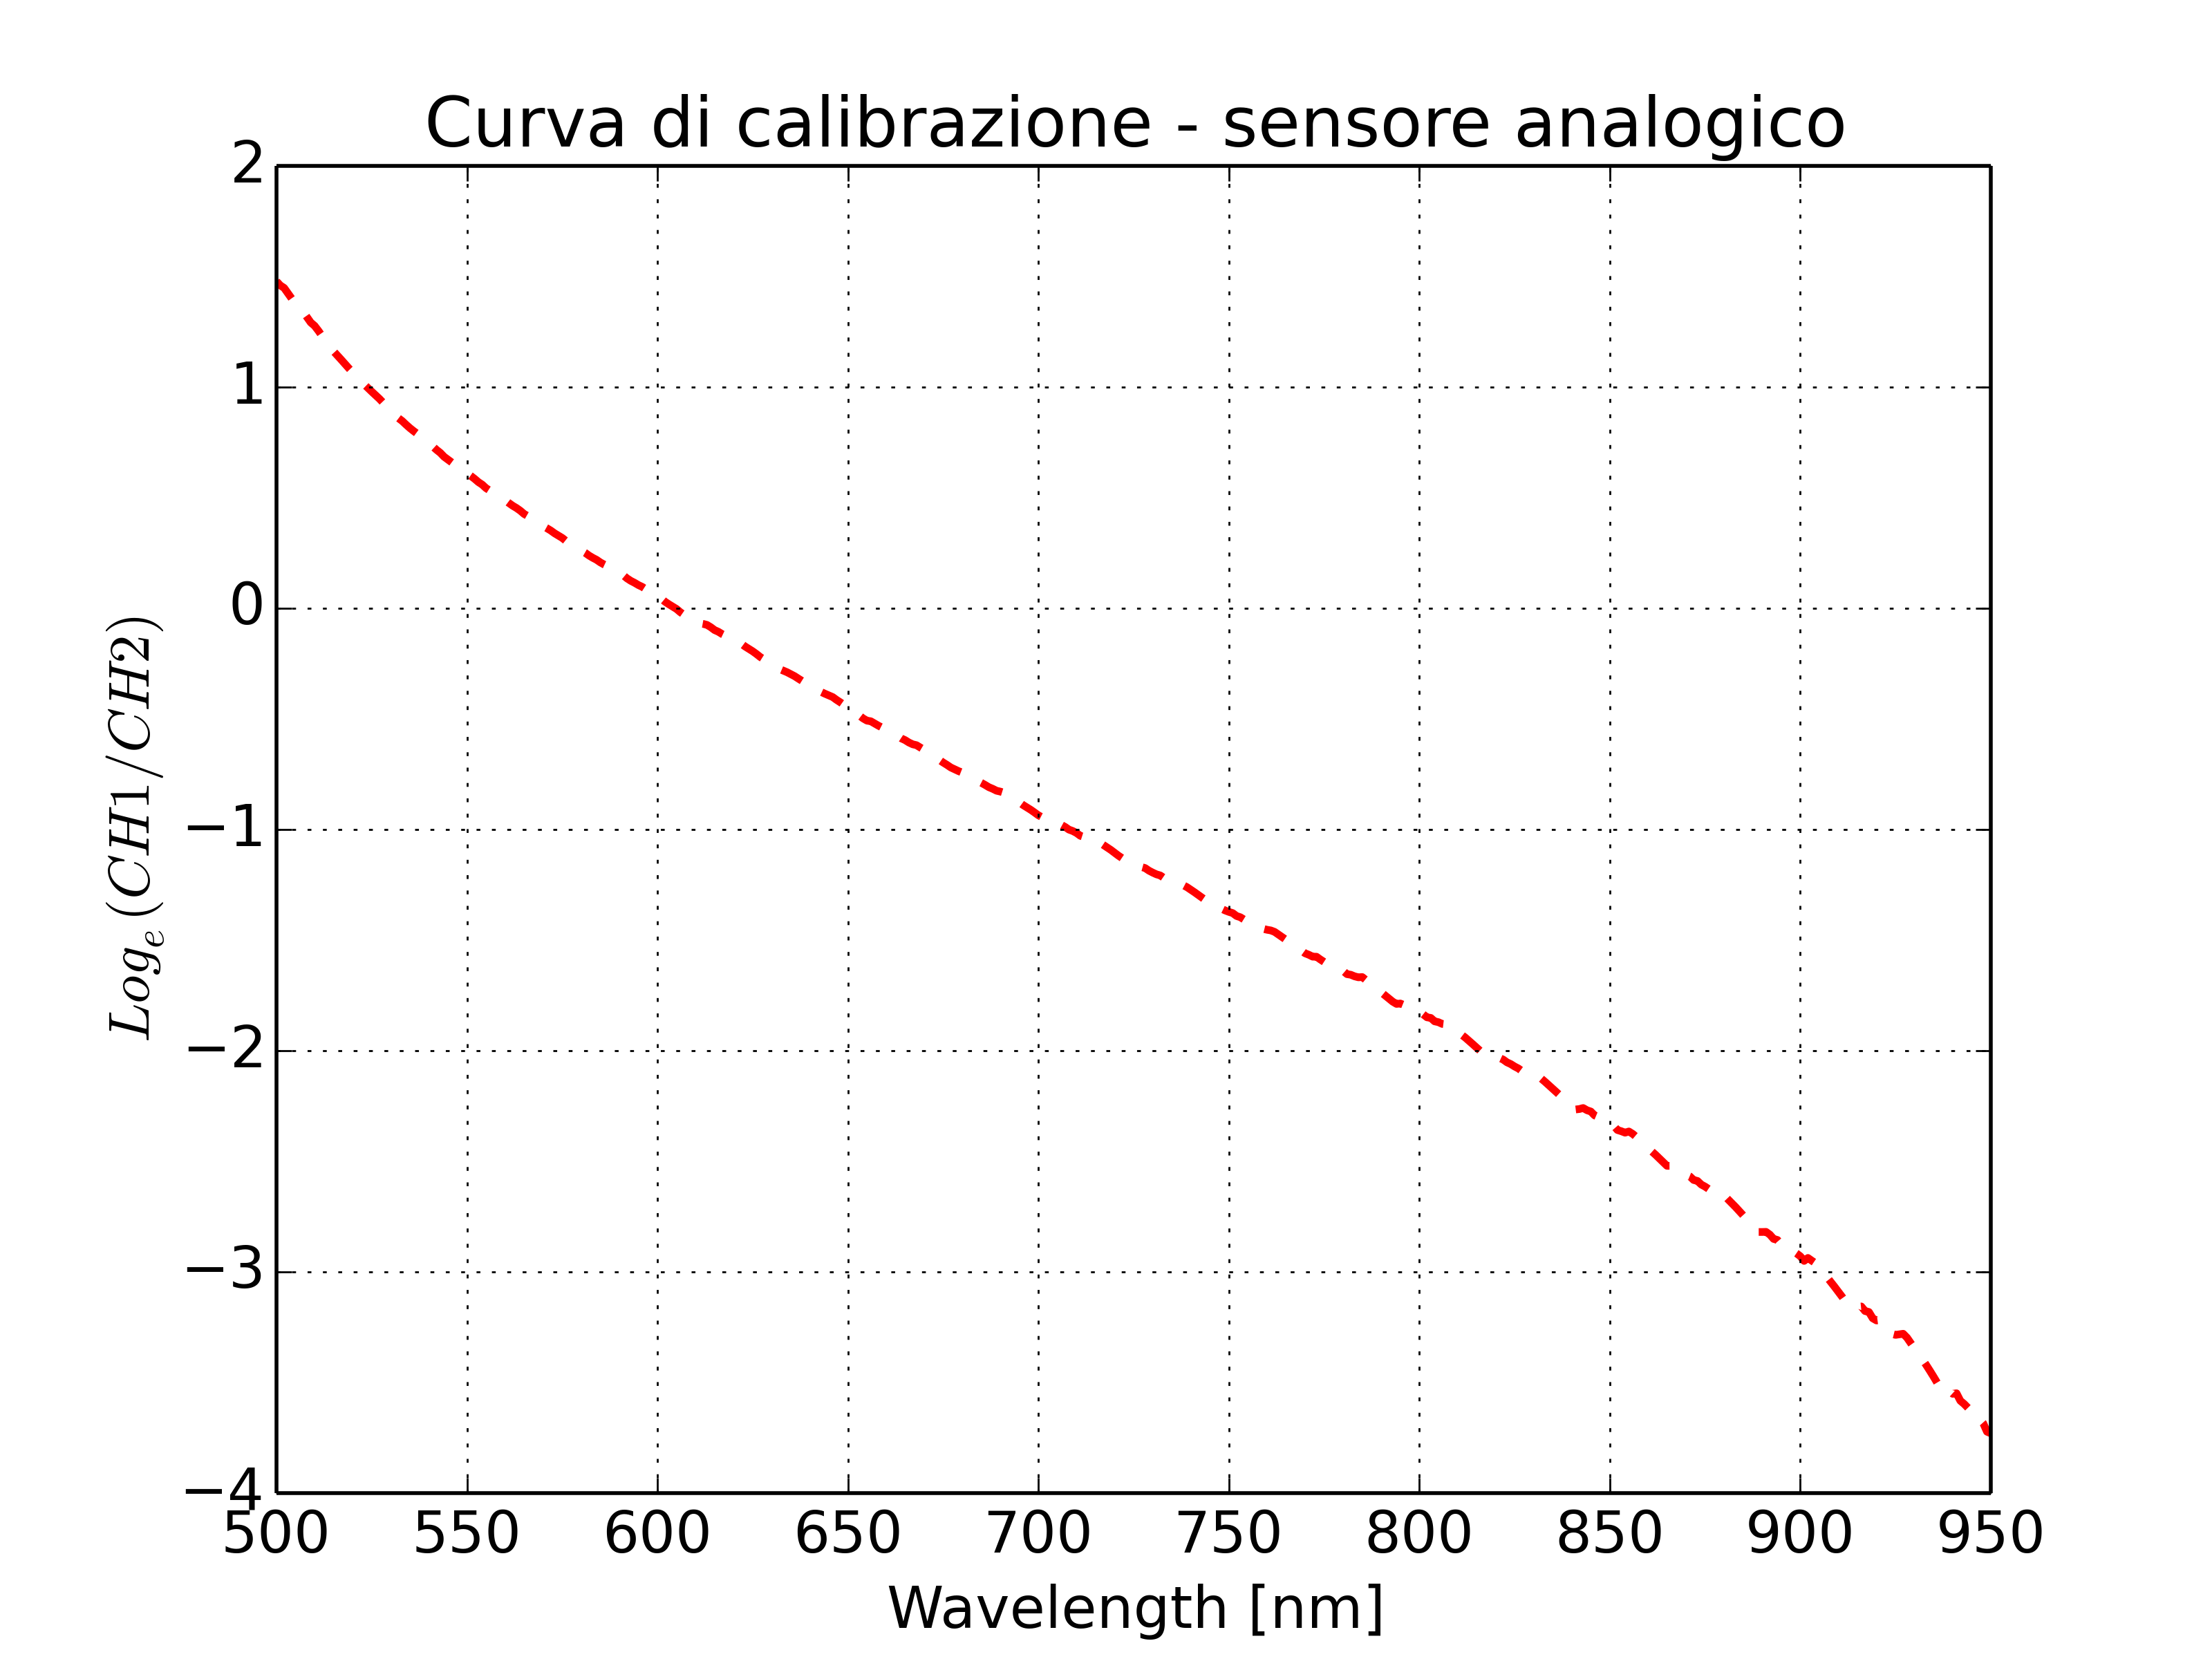
\includegraphics[width=0.8\linewidth]{./calibrazione_analog}
\caption{Curva di calibrazione del logaritmo del quoziente fra i segnali in funzione della lunghezza d'onda della radiazione.}
\label{fig:calibrazione_analog}
\end{figure}


Nella seguente tabella si riportano alcune fra le caratteristiche più rilevanti del \textsc{ws-7.56-to5}.

\begin{table}[h]
\centering
\begin{tabular}{c|c}
\hline Area attiva & 7.56$mm^2$ \\ 
 Range operativo $\lambda$ & 450-900 nm \\ 
 Risoluzione spettrale & 0.01 nm \\ 
 Livello di saturazione & 150 $\mu$W @0V \\ 
  & 3mW @5V \\ 
 Dark current  & 100 nA Max\\ 
  & 10 nA Typ \\
 Rise time & 1-10 $\mu$s (Diodo1-Diodo2) \\
 
\hline
\end{tabular} 
\end{table}
~\\

Poichè il sensore è composto da due fotodiodi, si deve montare un circuito con due op-amp in modalità invertente con due transimpedenze (eventualmente differenti); il catodo è a comune e andrà collegato ad entrambi gli ingressi non-invertenti, come mostrato nello schema in Figura (\ref{fig:circuito_analog}).\\

\begin{figure}
\centering
\subfloat[Subfigure 1 list of figures text][Schema di montaggio della coppia di fotodiodi del WS-756-TO5]{
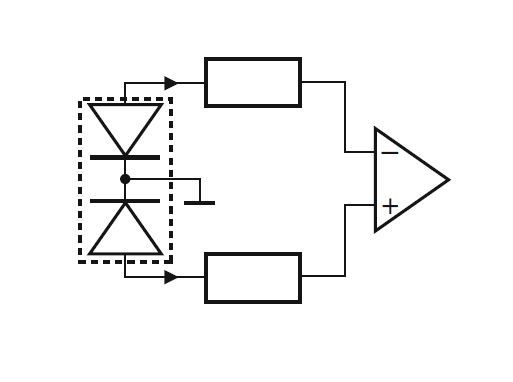
\includegraphics[width=0.5\linewidth]{./circuito_analog}
\label{fig:circuito_analog}}
%\qquad
\subfloat[Subfigure 2 list of figures text][Curva di responsività spettrale dei due diodi in funzione della lunghezza d'onda incidente.]{
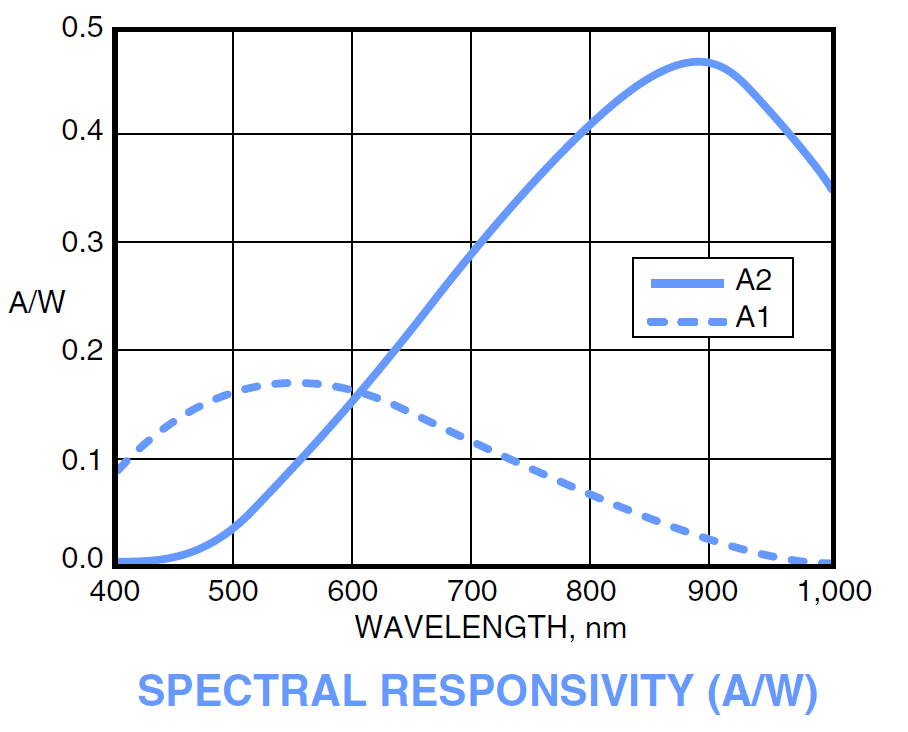
\includegraphics[width=0.6\linewidth]{./spectral_respo}
\label{fig:spectral_respo}}
%\qquad

\caption{}
\label{schema+respons}
\end{figure}



Per dimensionare opportunamente le trans-impedenze è sufficiente considerare la curva di responsività (Figura (\ref{fig:spectral_respo})) e stimare gli ordini di grandezza delle tensioni risultanti: infatti, come si evince dal grafico, per potenze incidenti limitate superiormente dal valore di saturazione (si prenda il caso non polarizzato), l'ordine di grandezza della corrente in uscita è delle decine, o al massimo centinaia, di $\mu$A. Affinchè si possano rivelare delle tensioni dell'ordine dei volt con i canali \textsc{CB33} e \textsc{CB65}, possiamo impiegare delle resistenze a trans-impedenza dell'ordine del centinaio di k$\Omega$. Le nostre prove sono state effettuate con $R_1 = 82.3 k\Omega$ e $R_2 = 82.2 k\Omega$ prima e $R_1 = 219 k\Omega$, $R_2 = 220 k\Omega$ poi.\\


Come prima acquisizione, mostriamo in Figura (\ref{fig:luce_stanza_enel}) il segnale prodotto dall'illuminazione ambientale della stanza, in cui è facilmente visibile la frequenza di 50Hz della rete elettrica (in realtà noi misuriamo 100Hz, il doppio, poichè l'intensità luminosa delle lampada va come il quadrato di $V_{ENEL}(t)$). Notiamo in particolare le tensioni negative, dovute all'uso dell'op-amp in modalità invertente come si vede dallo schema circuitale. Per verificare che le frequenze siano quelle previste, eseguiamo una veloce \textsc{fast-fourier transform} di entrambi i segnali dei canali, riportata in Figura (\ref{fig:fft_lucestanza}). Come si nota, avendo tolto il segnale di frequenza nulla, vi sono picchi nelle frequenze di armoniche multiple di 100Hz.

\begin{figure}
\centering
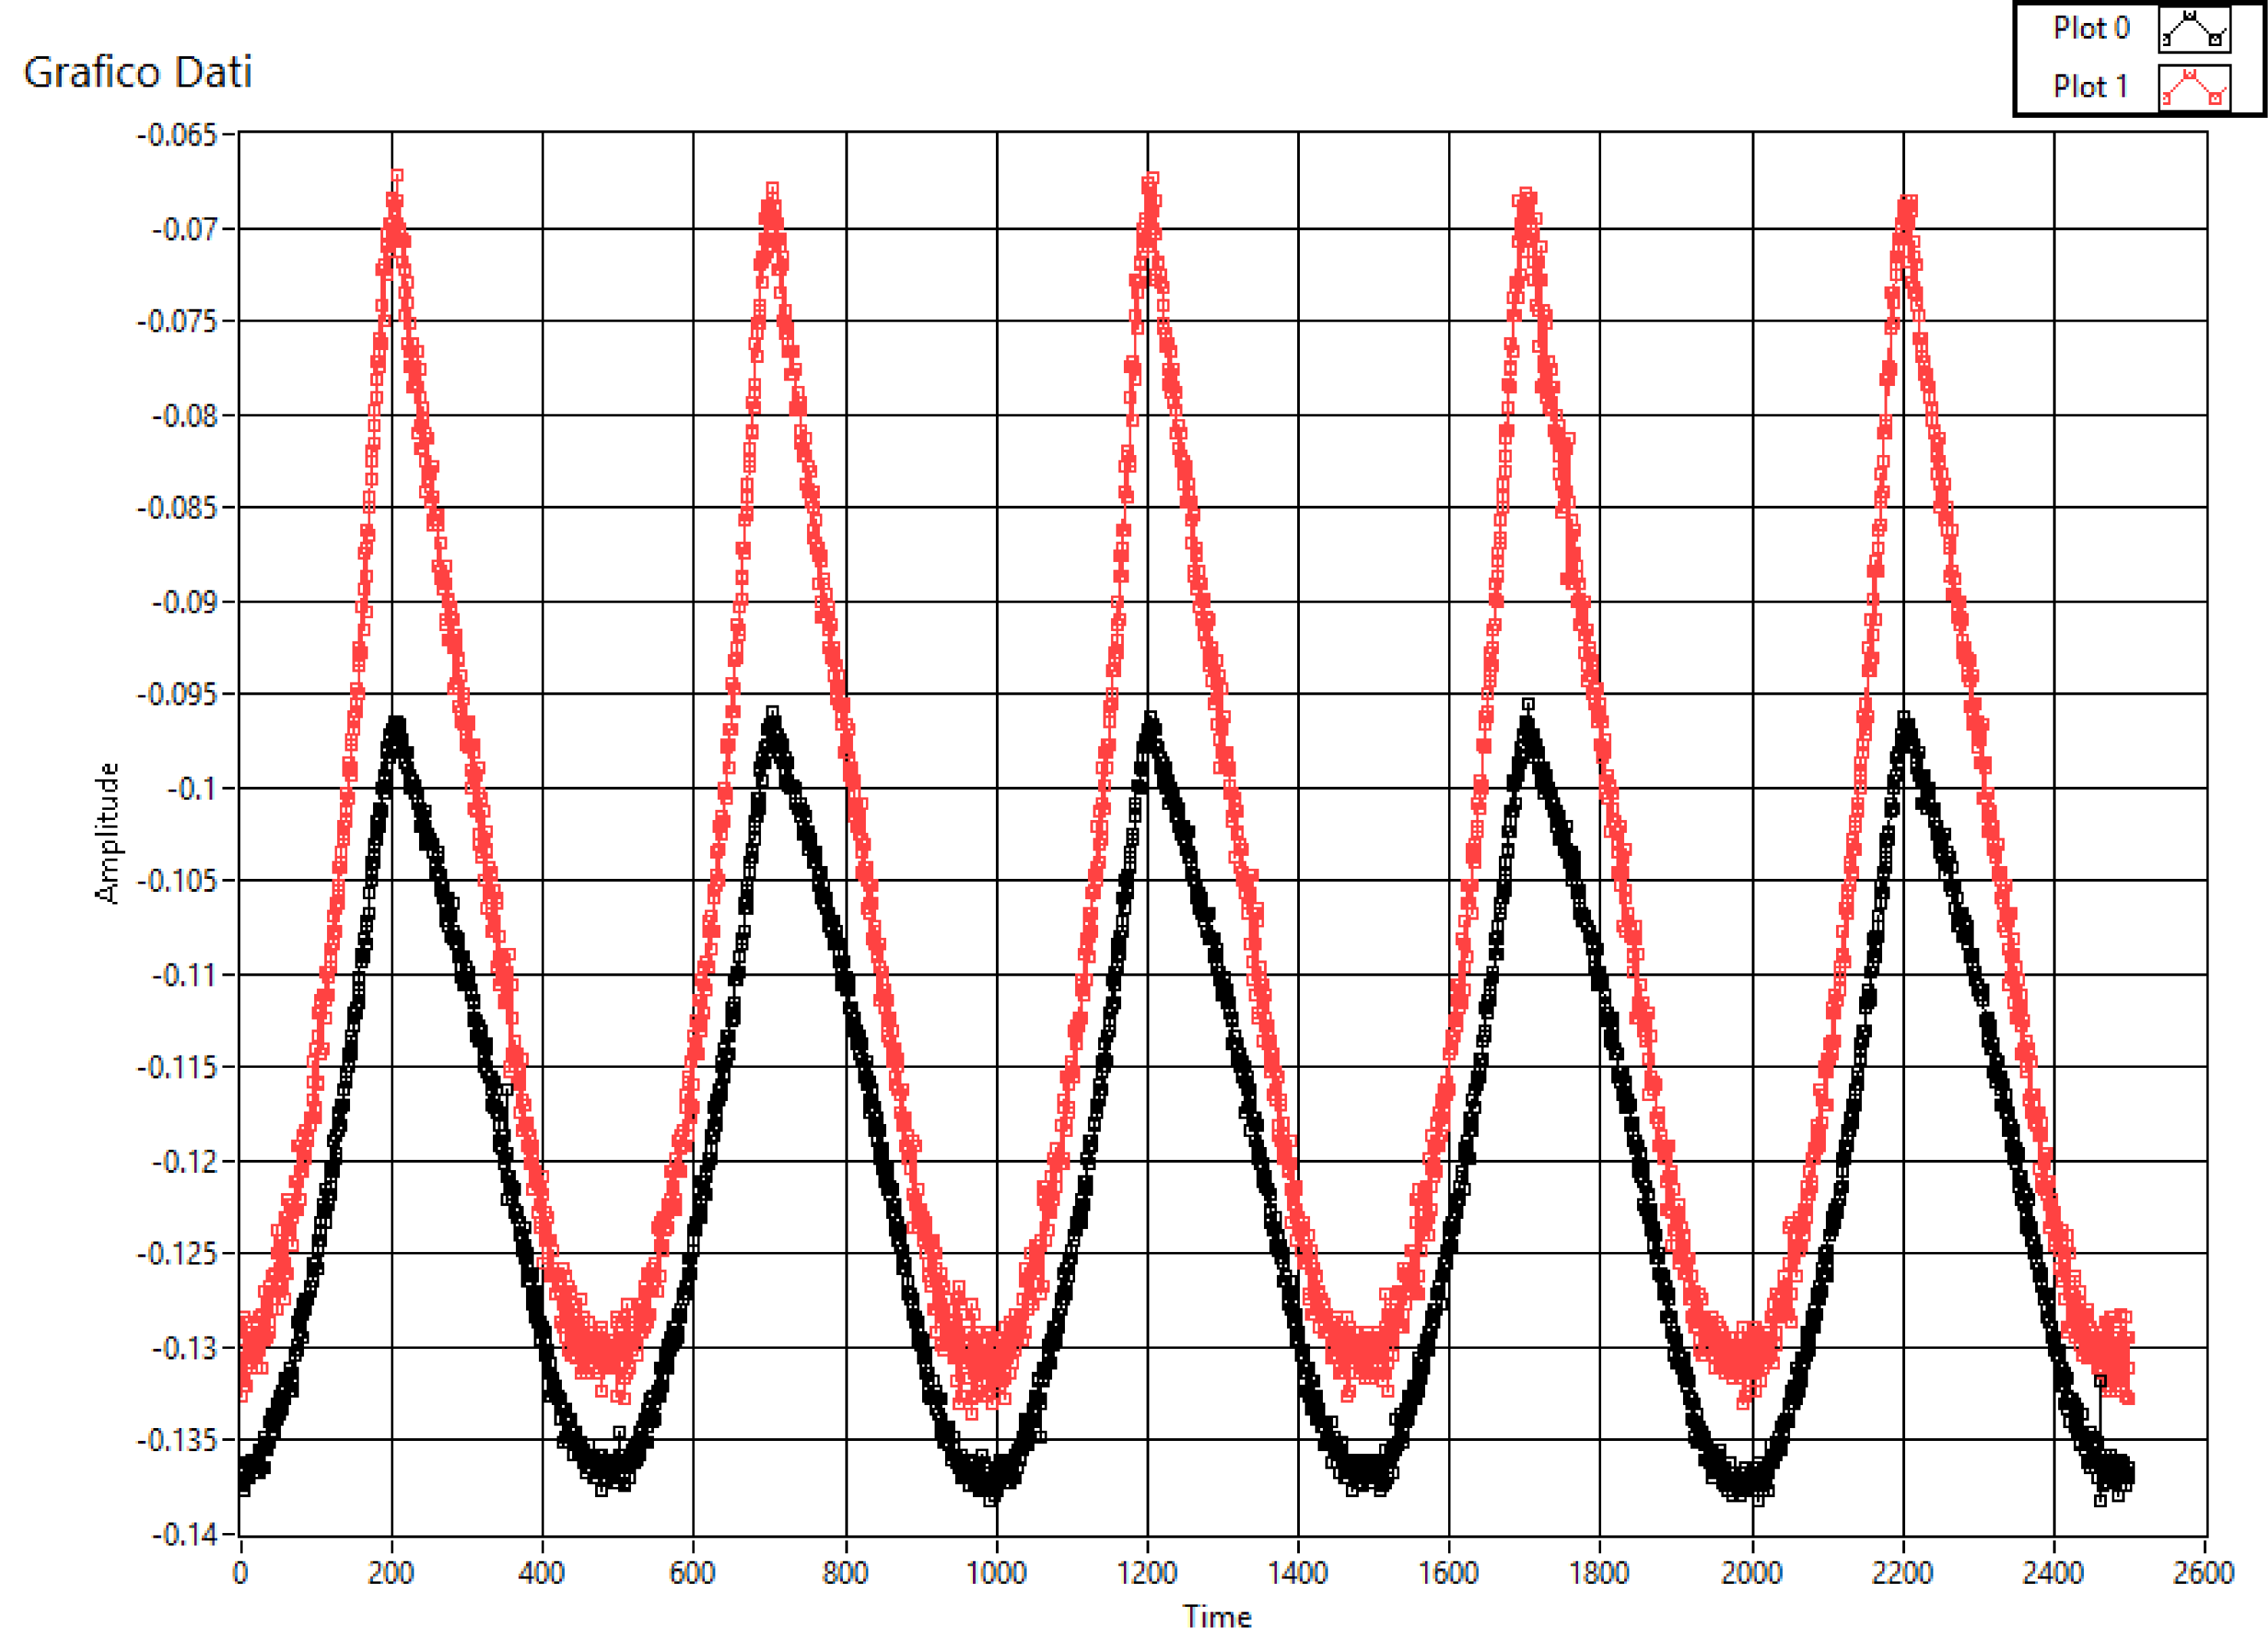
\includegraphics[width=0.7\linewidth]{./luce_stanza_enel}
\caption{Segnale relativo all'illuminazione della stanza data dalle lampade.}
\label{fig:luce_stanza_enel}
\end{figure}

\begin{figure}
\centering
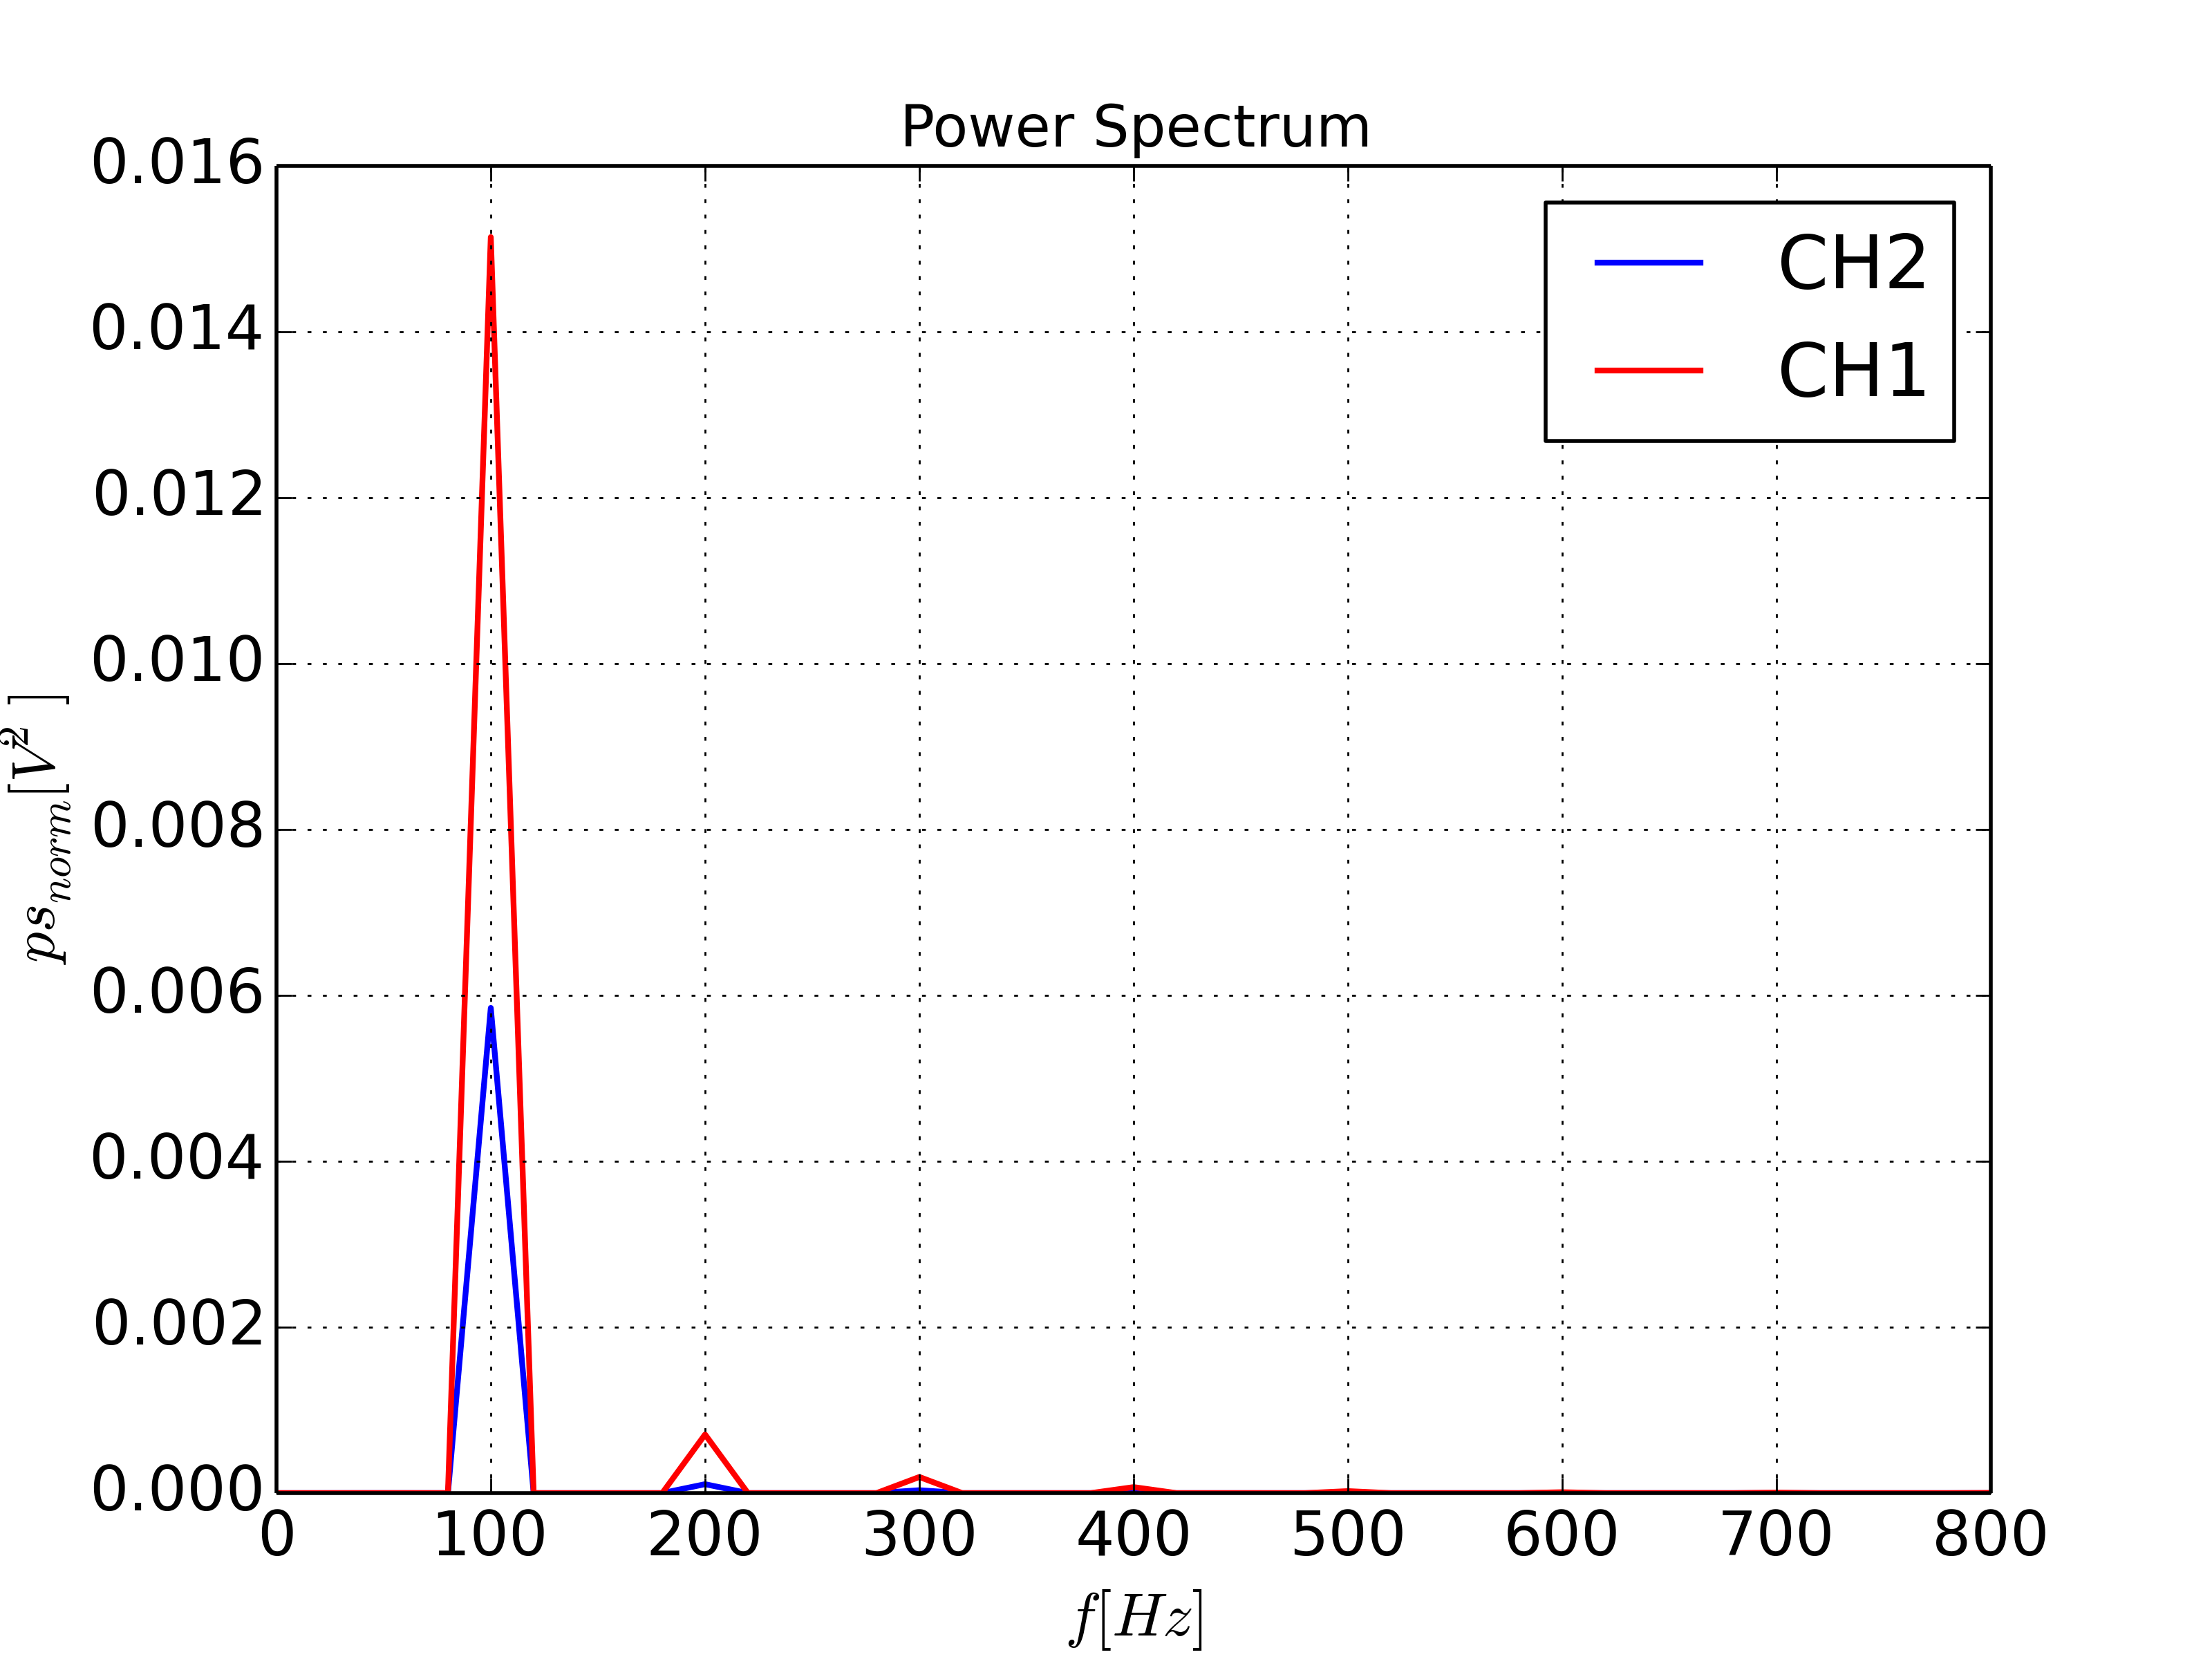
\includegraphics[width=0.7\linewidth]{./fft_lucestanza}
\caption{Fast Fourier transform del segnale di luce ambientale.}
\label{fig:fft_lucestanza}
\end{figure}


In condizioni di \textit{buio}, cioè in assenza di illuminazione e cercando di evitare fonti di calore che potrebbero essere rilevate come IR, la risposta in tensione è diversa da zero per entrambi i fotodiodi, poichè si attesta su un valore medio prossimo a 7-8mV, e sopratutto è positiva, contrariamente al comportamento del circuito in condizioni normali di lavoro ad esempio con la luce ambientale.\\
In particolare il segno diverso ci fa sospettare che possa trattarsi dell'effetto della corrente oscura (\textit{dark current}), dovuta al trasporto dei portatori di carica minoritari e che scorre dal catodo all'anodo di un dispositivo a semiconduttore, quindi nella direzione giusta per determinare l'effetto che stiamo osservando. Più precisamente: come riportato nella tabella con le specifiche tecniche del \textsc{ws-7.56-to5}, questo fotodiodo è caratterizzato da una dark current tipica di 10 nA, che, su una transimpedenza di 220 k$\Omega$ (circa), determina una tensione rilevata di 2.2mV, che è lo stesso ordine di grandezza del segnale di buio, ma corrisponde a circa un terzo di quello effettivamente rilevato. Tuttavia, grazie alla nostra ormai annuale esperienza con gli op-amp, siamo in grado di ipotizzare l'incidenza di un'altra grandezza: l'input offset current del \textsc{$\mu$a741cp} che come valore tipico riportato sul datasheet ha 20nA alle nostre condizioni di lavoro. Evidentemente il suo contributo si somma alla dark current, triplicando la tensione rilevata sulla transimpedenza per cui 220k$\Omega*30$nA $\simeq$ 7mV, molto vicino a quanto osservato.\\
Ad ogni modo, questo offset \textit{buio} non pregiudica in modo sostanziale le misure successive poichè si è cercato di rilevare tensioni di almeno 1-2 ordini di grandezza maggiori.\\

Può essere interessante discutere della possibilità di eliminare in maniera sistematica questo segnale dovuto al passaggio nella transimpedenza della dark current e dell'input offset current. Un modo che ci è sembrato abbastanza furbo consiste nell'impiegare un secondo sensore analogico \textbf{coperto} da collegare a polarità invertita alla transimpedenza: questi produrrà una sua propria dark current, sperabilmente molto prossima in valore a quella del sensore originario, ma in senso opposto, annullandone gli effetti. Il difetto principale di questa procedura sta nell'aver rinunciato a rimediare all'input offset current che quindi produrrà sempre un offset di tensione in uscita. O si tiene conto di ciò nel trattamento dei dati, compensando artificialmente per la tensione mancante, che però sotto condizioni differenti di lavoro e di alimentazione potrebbe variare, oppure si introduce un circuito sommatore a valle dell'op-amp che riceve in ingresso il segnale originario più quello prodotto da un ulteriore op-amp con una transimpedenza dello stesso valore.\\ 

\subsection{Caratterizzazione dei LED}
Mettiamo alla prova il nostro rilevatore con (tutti) i LED a disposizione del laboratorio. Ogni LED è stato posto in corrispondenza dell'area esposta della giunzione e quanto meglio isolato dall'illuminazione esterna della stanza; quindi sono state acquisiti per ciascuno circa $10^4$ campionamenti con il VI \textsc{acquis\_base2}, da cui è stata calcolata la media aritmetica e lo scarto quadratico medio. Per ciascuno di essi è stato estratto il valore del logaritmo dei rapporti fra i due segnali (come spiegato nell'introduzione al sensore analogico) e plottati insieme alla curva di calibrazione del \textsc{ws-7.56-to5}, in modo da verificare se la lunghezza d'onda stimata a partire da tale curva coincida con quella effettiva riportata sul datasheet. Nella Tabella (\ref{tabella_LED}) vengono riassunti i LED impiegati e le loro $\lambda$ di fabbrica, ove disponibili.

\begin{table}[h]
\centering
% This LaTeX table template is generated by emacs 24.3.1
\begin{tabular}{l|c|c|c}
\hline
\textbf{LED} & \textbf{Wavelength} (nm) & $log(CH1/CH2)$ & $\delta log$ \\
\hline
\textsc{hlmpd101-645} & 645 & -0.539 & 0.006 \\
\textsc{hlmpc115-red} & 637 & -0.522 & 0.003 \\
\textsc{hlmpc315-Y} & 585 & 0.172 & 0.006 \\
\textsc{la3366} & 615 & -0.101 & 0.003 \\
\textsc{lb3333} & 470 & 2.26 & 0.02 \\
\textsc{led450} & 450 & 2.87 & 0.02 \\
\textsc{lo3336} & 606 & -0.101 & 0.002 \\
\textsc{lpk376} & 560 & 0.65 & 0.04 \\
\textsc{ls3336} & 633 & -0.332 & 0.001 \\
\textsc{lt3333} & 528 & 0.908 & 0.01 \\
\textsc{ly3336} & 587 & 0.209 & 0.001 \\
\textsc{sfh4873-880} & 880 & -2.439 & 0.004 \\
\textsc{ssl-lxa} & 660 & -0.58 & 0.02 \\
\textsc{tshg8400-830} & 830 & -1.964 & 0.007 \\
\hline
\end{tabular}
\caption{title}
\label{tabella_LED}
\end{table}
~\\


Si riporta in Figura (\ref{fig:calibrazione_led}) il grafico con il logaritmo del rapporto $CH1/CH2$ dei LED in funzione di $\lambda$, insieme con i punti della curva di calibrazione. Come si può notare, in generale l'accordo è piuttosto buono con i punti di calibrazione: stimiamo che non vi siano più di una ventina di nm di differenza fra i punti corrispondenti ai LED e la curva. Rileviamo, inoltre, due punti sperimentali dei LED blu \textsc{lb3333} e \textsc{led450} che si trovano a lunghezze d'onda inferiori al limite minimo della curva di calibrazione, ma posizionati in modo tale da disporsi abbastanza bene lungo un prolungamento ideale di tale curva.\\



Vogliamo essere più quantitativi, perciò per valutare in maniera più precisa lo scarto fra $\lambda_{THEO}$ (che sarebbe quella di fabbrica) e la $\lambda_{CAL}$, cioè quella che risulterebbe dal $log(CH1/CH2)$ secondo la calibrazione, è possibile scrivere un semplice algoritmo che colloca il log del rapporto lungo la curva, per estrapolare $\lambda_{CAL}$. Nel grafico in Figura (\ref{fig:LED_confronto}), viene plottato lo scarto fra queste due lunghezze d'onda per ciascun LED. Per quanto riguarda i LED nel blu, si tenga presente che lo scarto calcolato è quello fra $\lambda_{THEO}$ e il valore minimo di $\lambda$ dato dalla curva di calibrazione, pari a 500nm: supponiamo che l'accordo possa essere molto migliore se avessimo dei dati per lunghezze d'onda inferiori.\\


\begin{figure}
\centering
\subfloat[Subfigure 1 list of figures text][Dispersione dei LED sulla curva di calibrazione del sensore analogico.]{
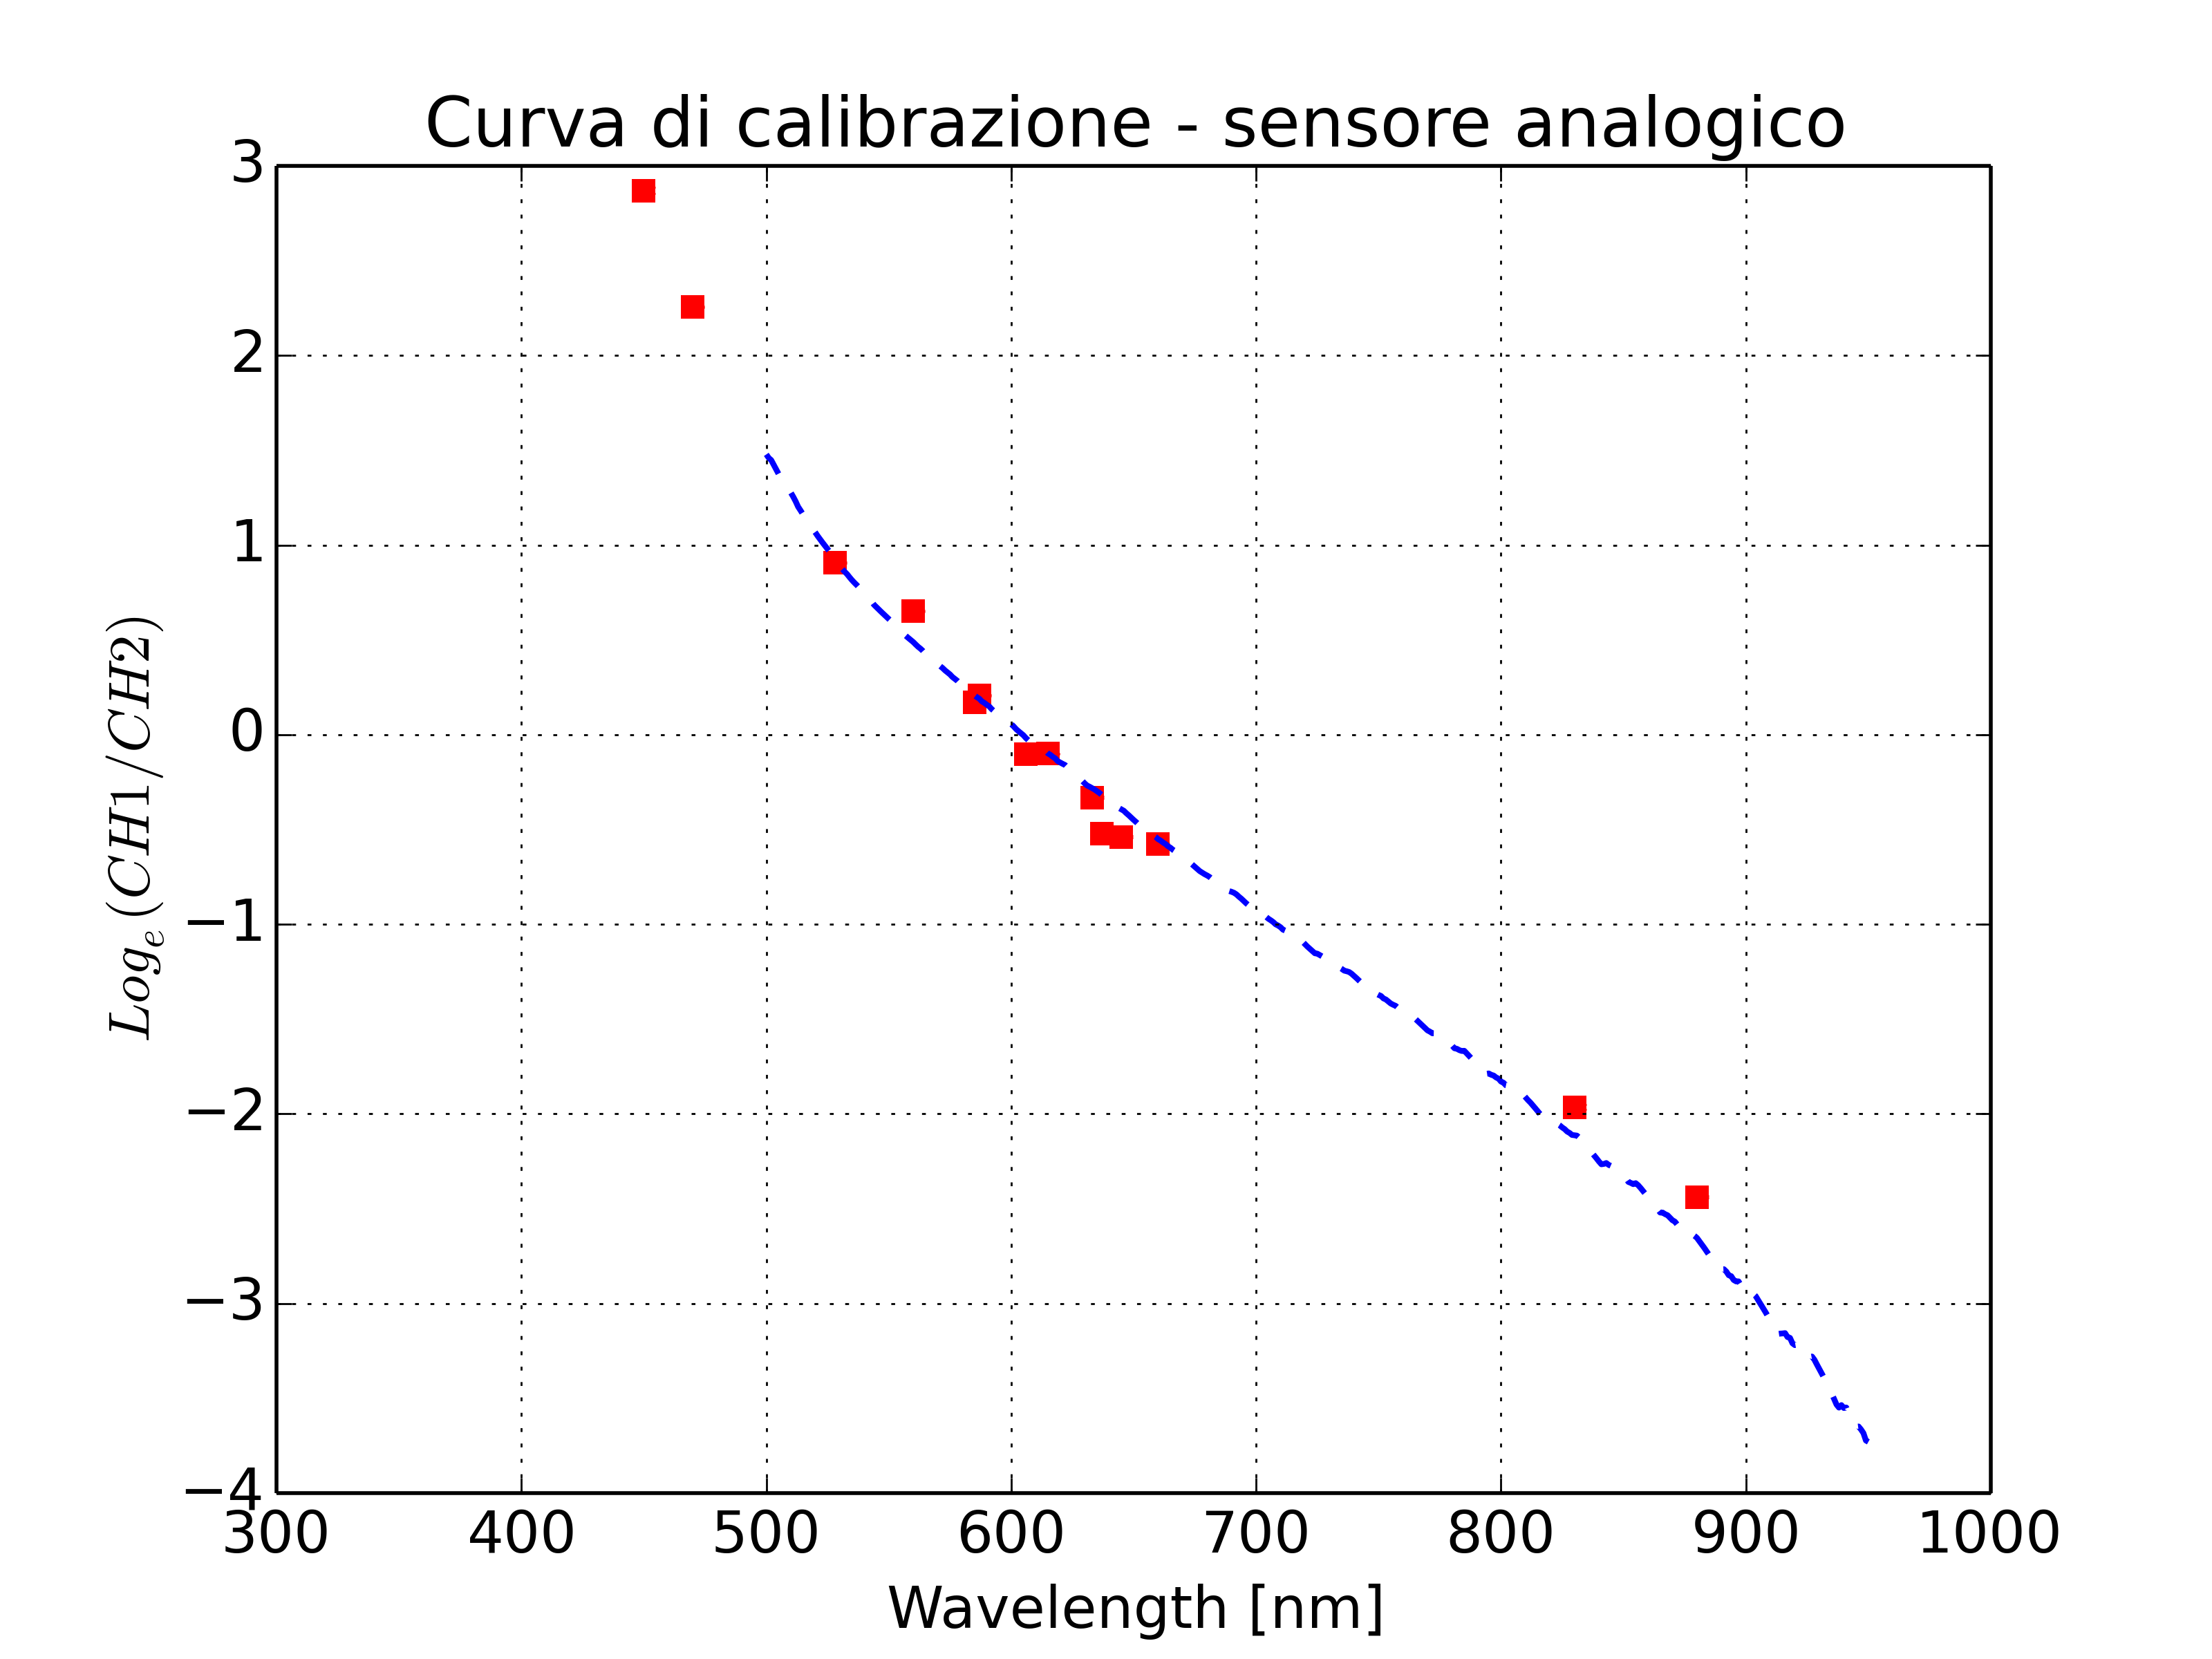
\includegraphics[width=0.6\linewidth]{./calibrazione_led}
\label{fig:calibrazione_led}}
%\qquad
\subfloat[Subfigure 2 list of figures text][Scarto fra lunghezze d'onda di "fabbrica" e da "calibrazione" per ciascun LED.]{
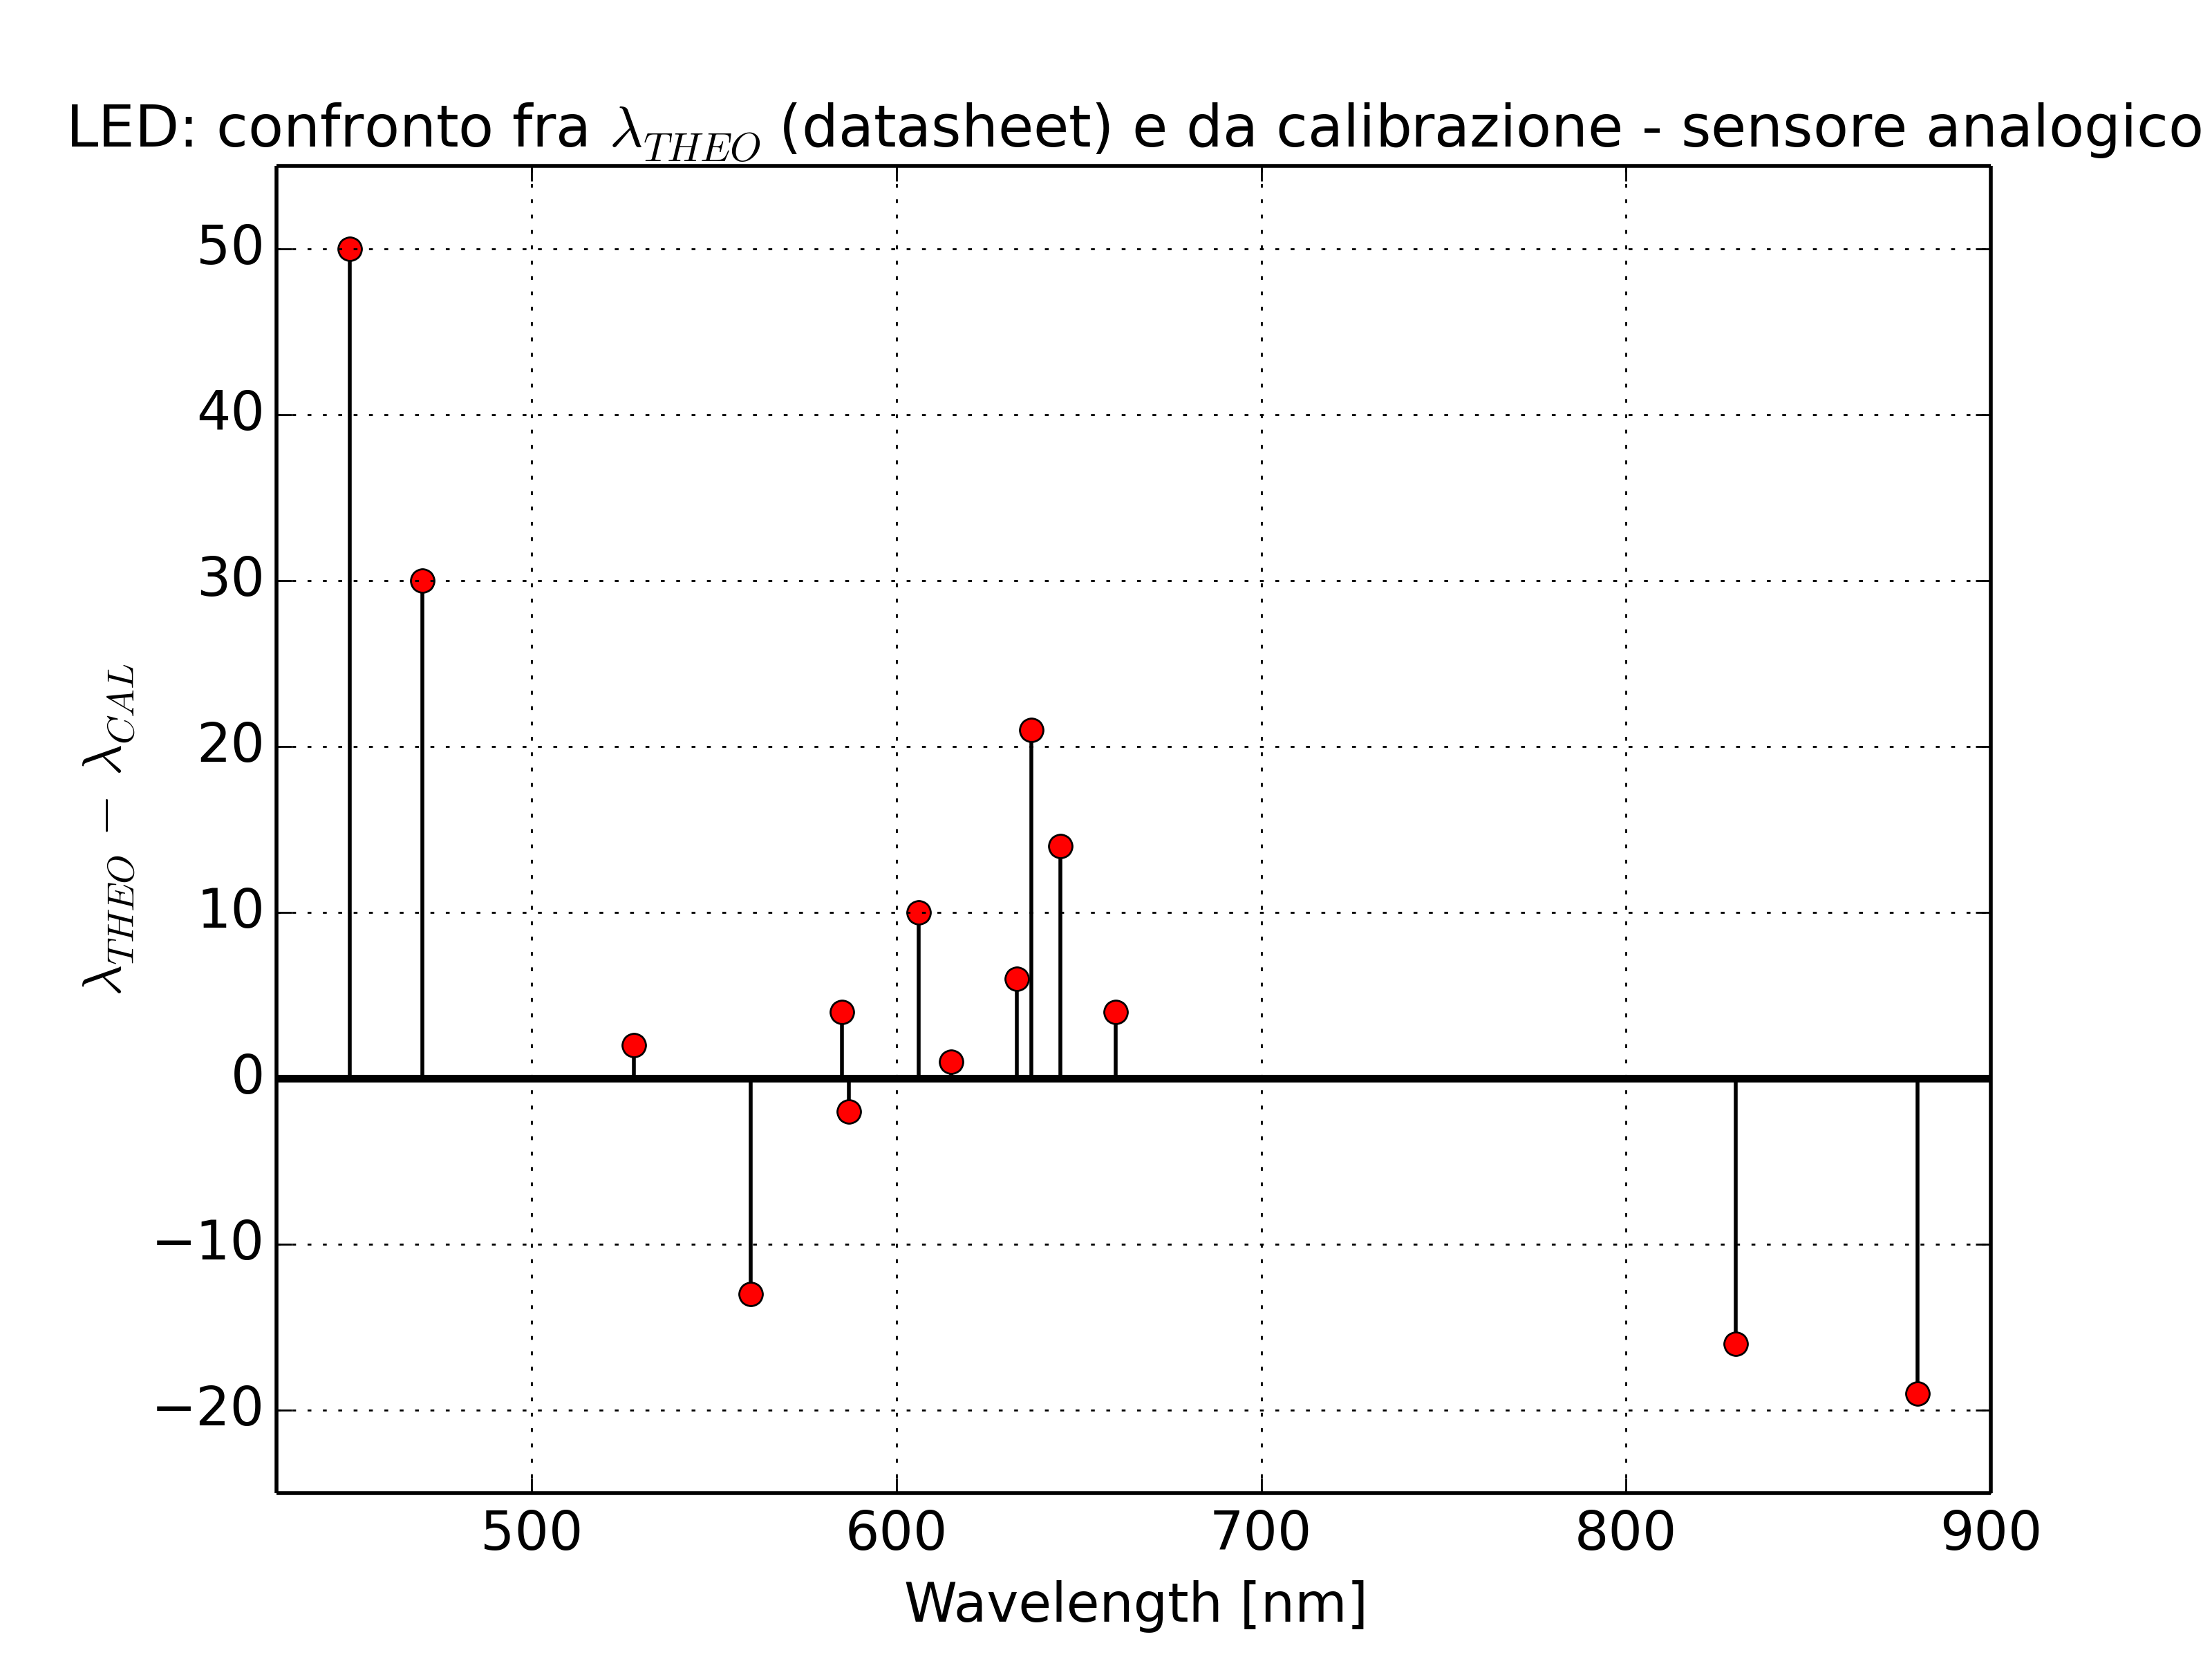
\includegraphics[width=0.6\linewidth]{./LED_confronto}
\label{fig:LED_confronto}}
%\qquad

\caption{Rilevazione della lunghezza d'onda dei LED e confronto con il valore atteso.}
\label{LED_wavel}
\end{figure}

\subsection{Caratterizzazione dei colori RGB di un monitor}
Riproponendo la stessa analisi effettuata con l'integrato \textsc{apds-9301}, e con le stesse condizioni di lavoro per lo script che riproduce i colori sul monitor in uso \footnote{300 triplette RGB intervallate l'una dall'altra da 0.1s}, cerchiamo di rilevare ancora una volta le lunghezze d'onda \textit{effettive} dei colori mostrati su schermo. In Figura (\ref{fig:analog_monitor_colori}) sono plottati i segnali di tensione sui due canali in funzione del tempo. Si ricorda che le triplette RGB generate dallo script sono della forma seguente:

\begin{table}[h]
\centering
\begin{tabular}{c|c|c}
 \textbf{R} &\textbf{ G} & \textbf{B} \\ 
 \hline 1 & 0 & 0 \\ 
 1 & 0.1 & 0 \\ 
 1 & 0.2 & 0 \\ 
 . & . & . \\ 

 1 & 1 & 0 \\ 
 0.9 & 1 & 0 \\ 
 0.8 & 1 & 0 \\ 
 . & . & . \\ 
 0 & 1 & 0 \\ 
 0 & 1 & 0.1 \\
\end{tabular}
\quad
\begin{tabular}{c|c|c}

 0 & 1 & 0.2 \\ 
 . & . & . \\ 

 0 & 1 & 1 \\ 
 0 & 0.9 & 1 \\ 
 . & . & . \\ 
 0 & 0 & 1 \\ 
 0.1 & 0 & 1 \\ 
 . & . & . \\ 
 1 & 0 & 1 \\ 
 . & . & . \\ 
\hline 
\end{tabular} 
\end{table}
~\\

cioè non vi sono mai tutti e tre i LED accesi contemporaneamente, ma solo due per volta.  Le tensioni sono negative (per l'uso invertente dell'op-amp) per cui per ritrovare la familiare forma dell'esperienza della week-09 (se la numerazione è corretta) bisogna immaginarle ribaltate. I picchi negativi corrispondono alle situazioni di RGB del tipo (110, 101, 011), quelle in cui due LED sono accesi contemporanemante al massimo della loro intensità. Le \textit{valli} (immaginando ribaltata l'immagine) sono invece relate alle triplette pure (100, 010, 001), quindi solo rosso, verde o blu in quest'ordine. Si noti come il segnale del CH2 (in rosso) nel grafico, ha una risposta molto marcata sul rosso (colore), maggiore di quella del CH1 (plot bianco) che invece prevale sul verde e sul blu. Questo è in linea con quanto ci aspettavamo a partire dallo studio del grafico della responsività spettrale riportato in Figura (\ref{fig:spectral_respo}).\\

\begin{figure}
\centering
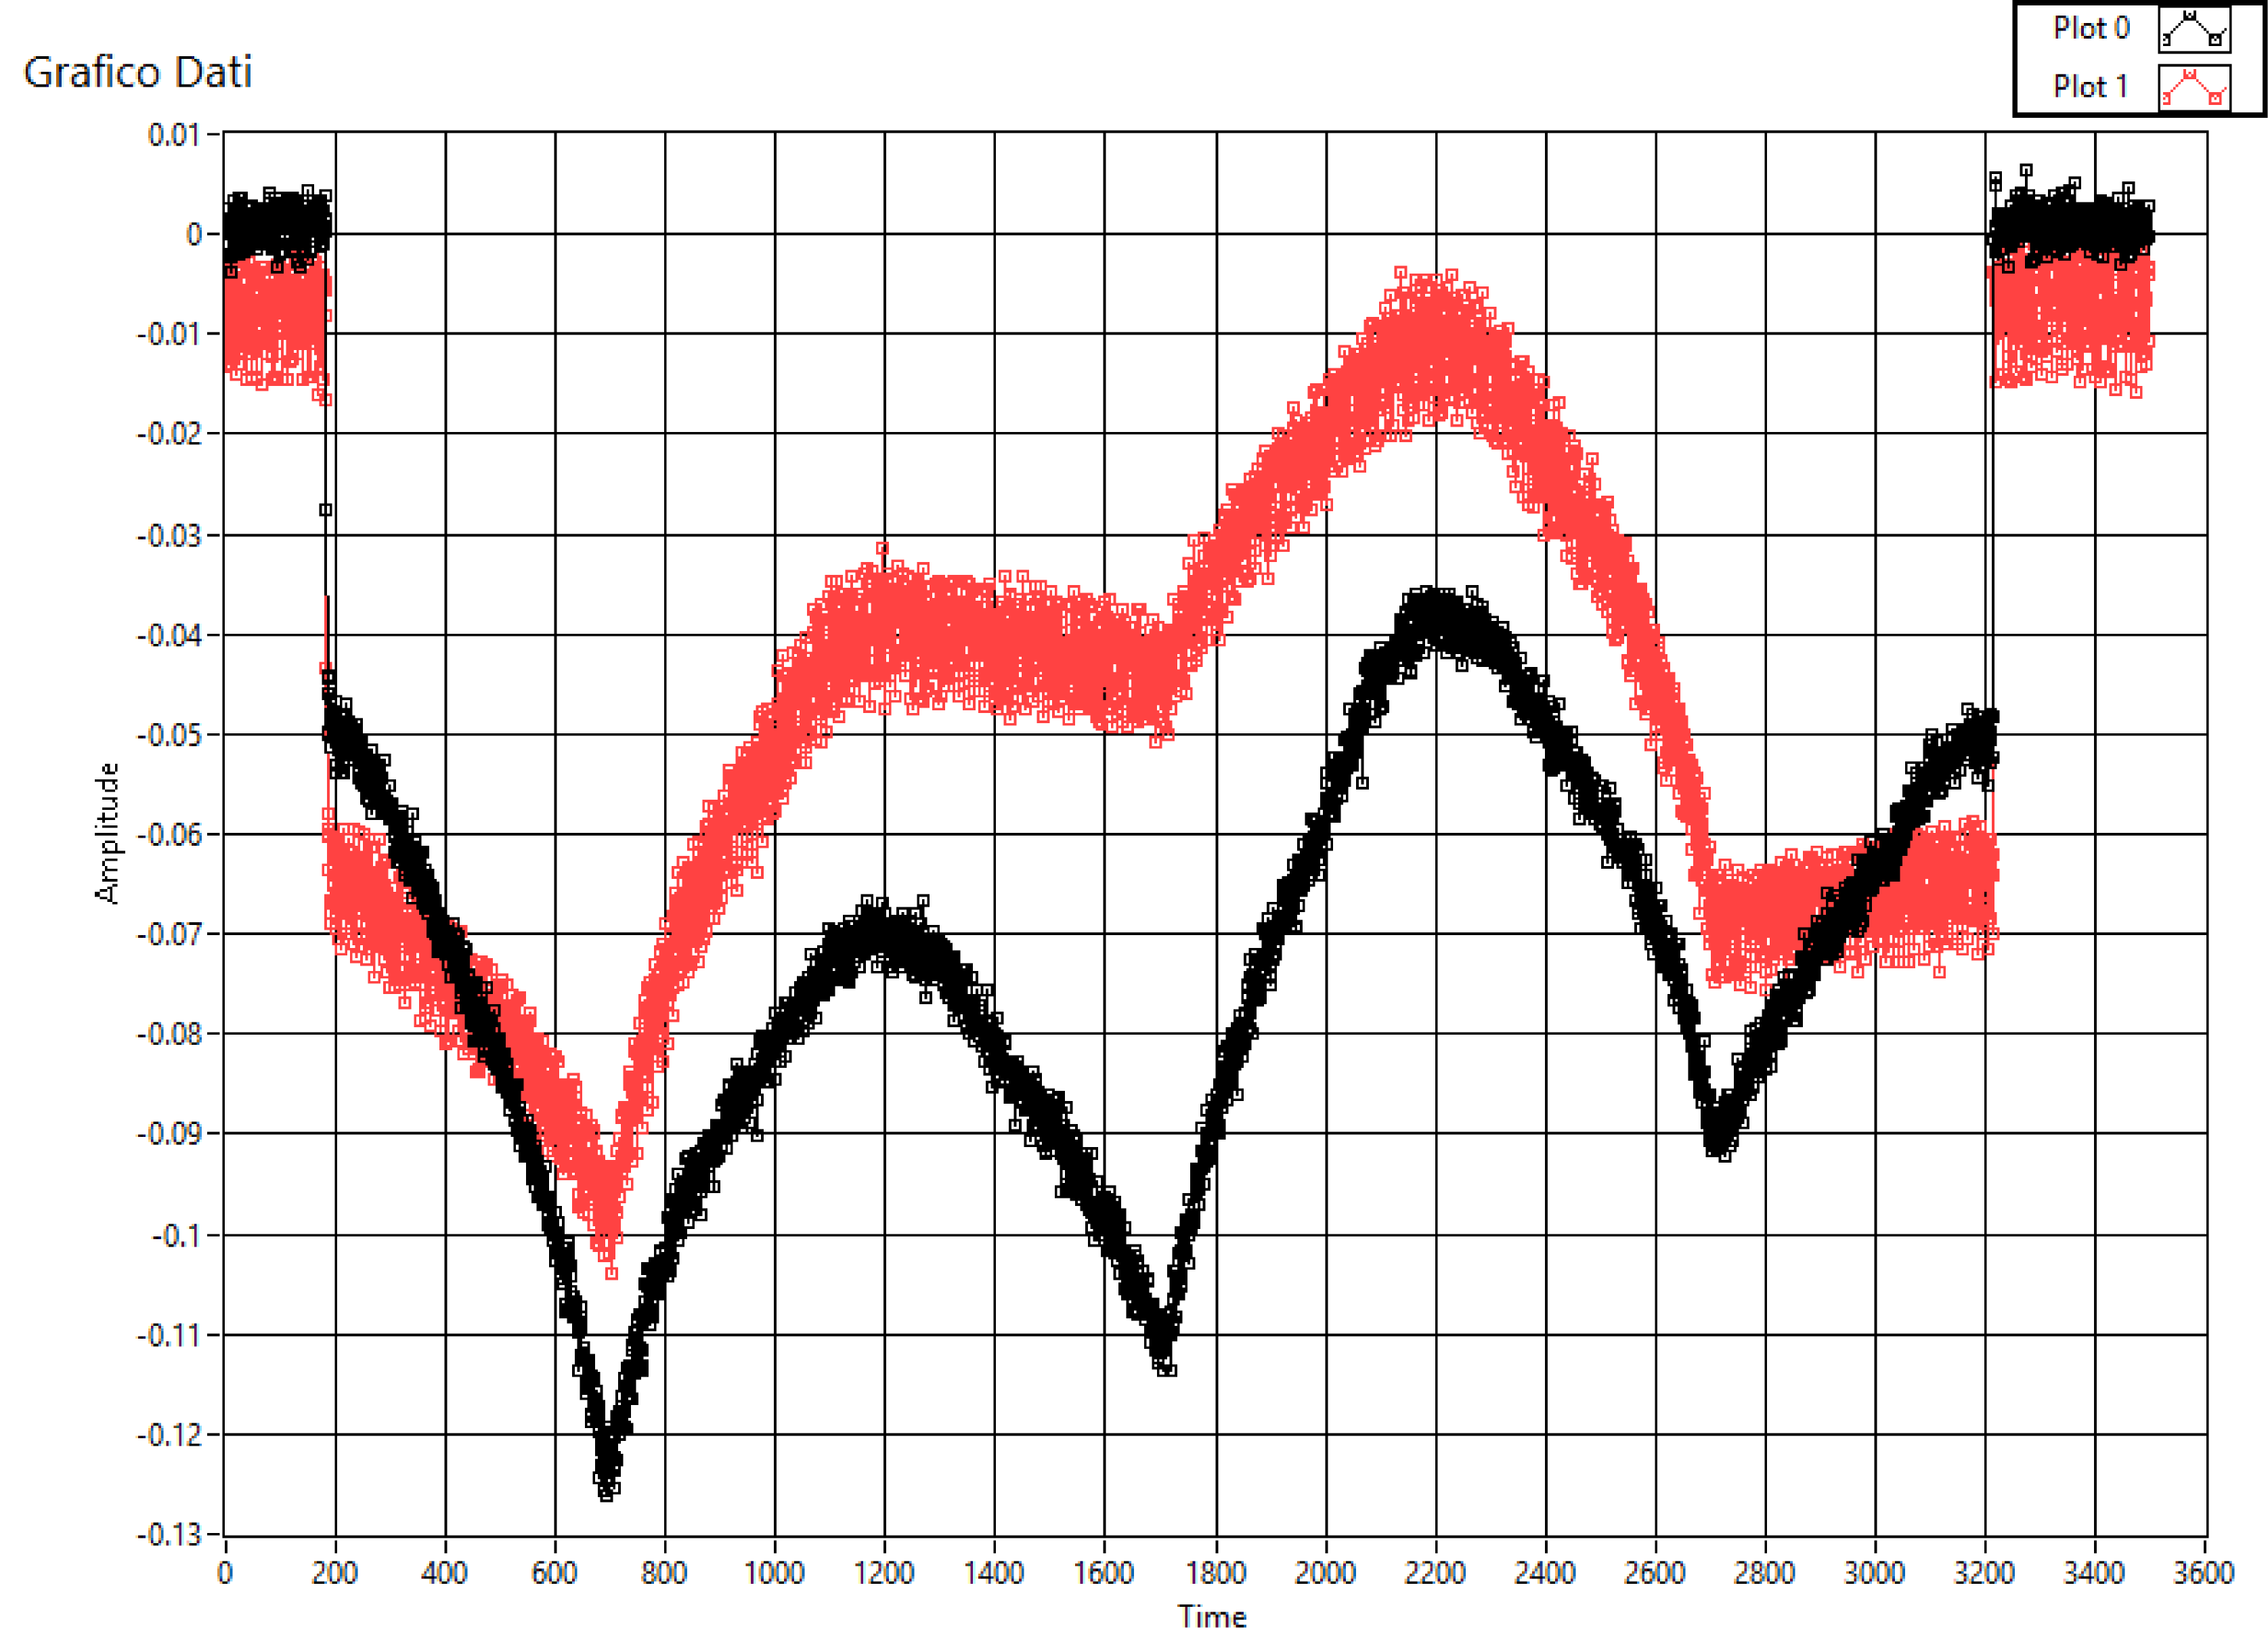
\includegraphics[width=0.7\linewidth]{./analog_monitor_colori}
\caption{Segnali di tensione dei due canali CH1, CH2 durante lo svolgimento dello script.}
\label{fig:analog_monitor_colori}
\end{figure}


Un'ulteriore caratteristica del plot è la sua evidente \textit{rumorosità}, vale a dire la dispersione piuttosto ampia delle tensioni in un breve intervallo di tempo: i parametri di acquisizione del segnale sono stati settati in modo da ottenere 10 acquisizioni per ogni tripletta RGB mostrata su schermo. Una spiegazione di questo fenomeno può essere dovuta ai microspostamenti del sensore che inevitabilmente sono avvenuti durante l'acquisizione (il sensore era mantenuto a diretto contatto con lo schermo), che possono aver introdotto delle interferenze da parte della luce ambientale, così come la familiare distorsione cromatica che si verifica quando viene esercitata della pressione su delle porzioni di monitor LCD, che potrebbero aver reso il colore disomogeneo.\\



Risulta naturale, a questo punto, ripulire il segnale mediando su queste dieci misure per ottenere dei rapporti CH1/CH2 puliti. Il risultato è in Figura (\ref{fig:analog_segnale_log_average}) dove, sulla scala di sinistra, vi sono le tensioni e i punti sperimentali sono provvisti di errore (scarto quadratico medio), mentre sulla scala di destra in blu vi è il logaritmo del rapporto. Sappiamo, dalla calibrazione del sensore, che valori alti del $log(CH1/CH2)$ corrispondono a lunghezze d'onda minori, per cui indicativamente verifichiamo che procedendo dal rosso al blu $\lambda$ diminuisce per poi riaumentare tornando sul rosso.\\


\begin{figure}
\centering
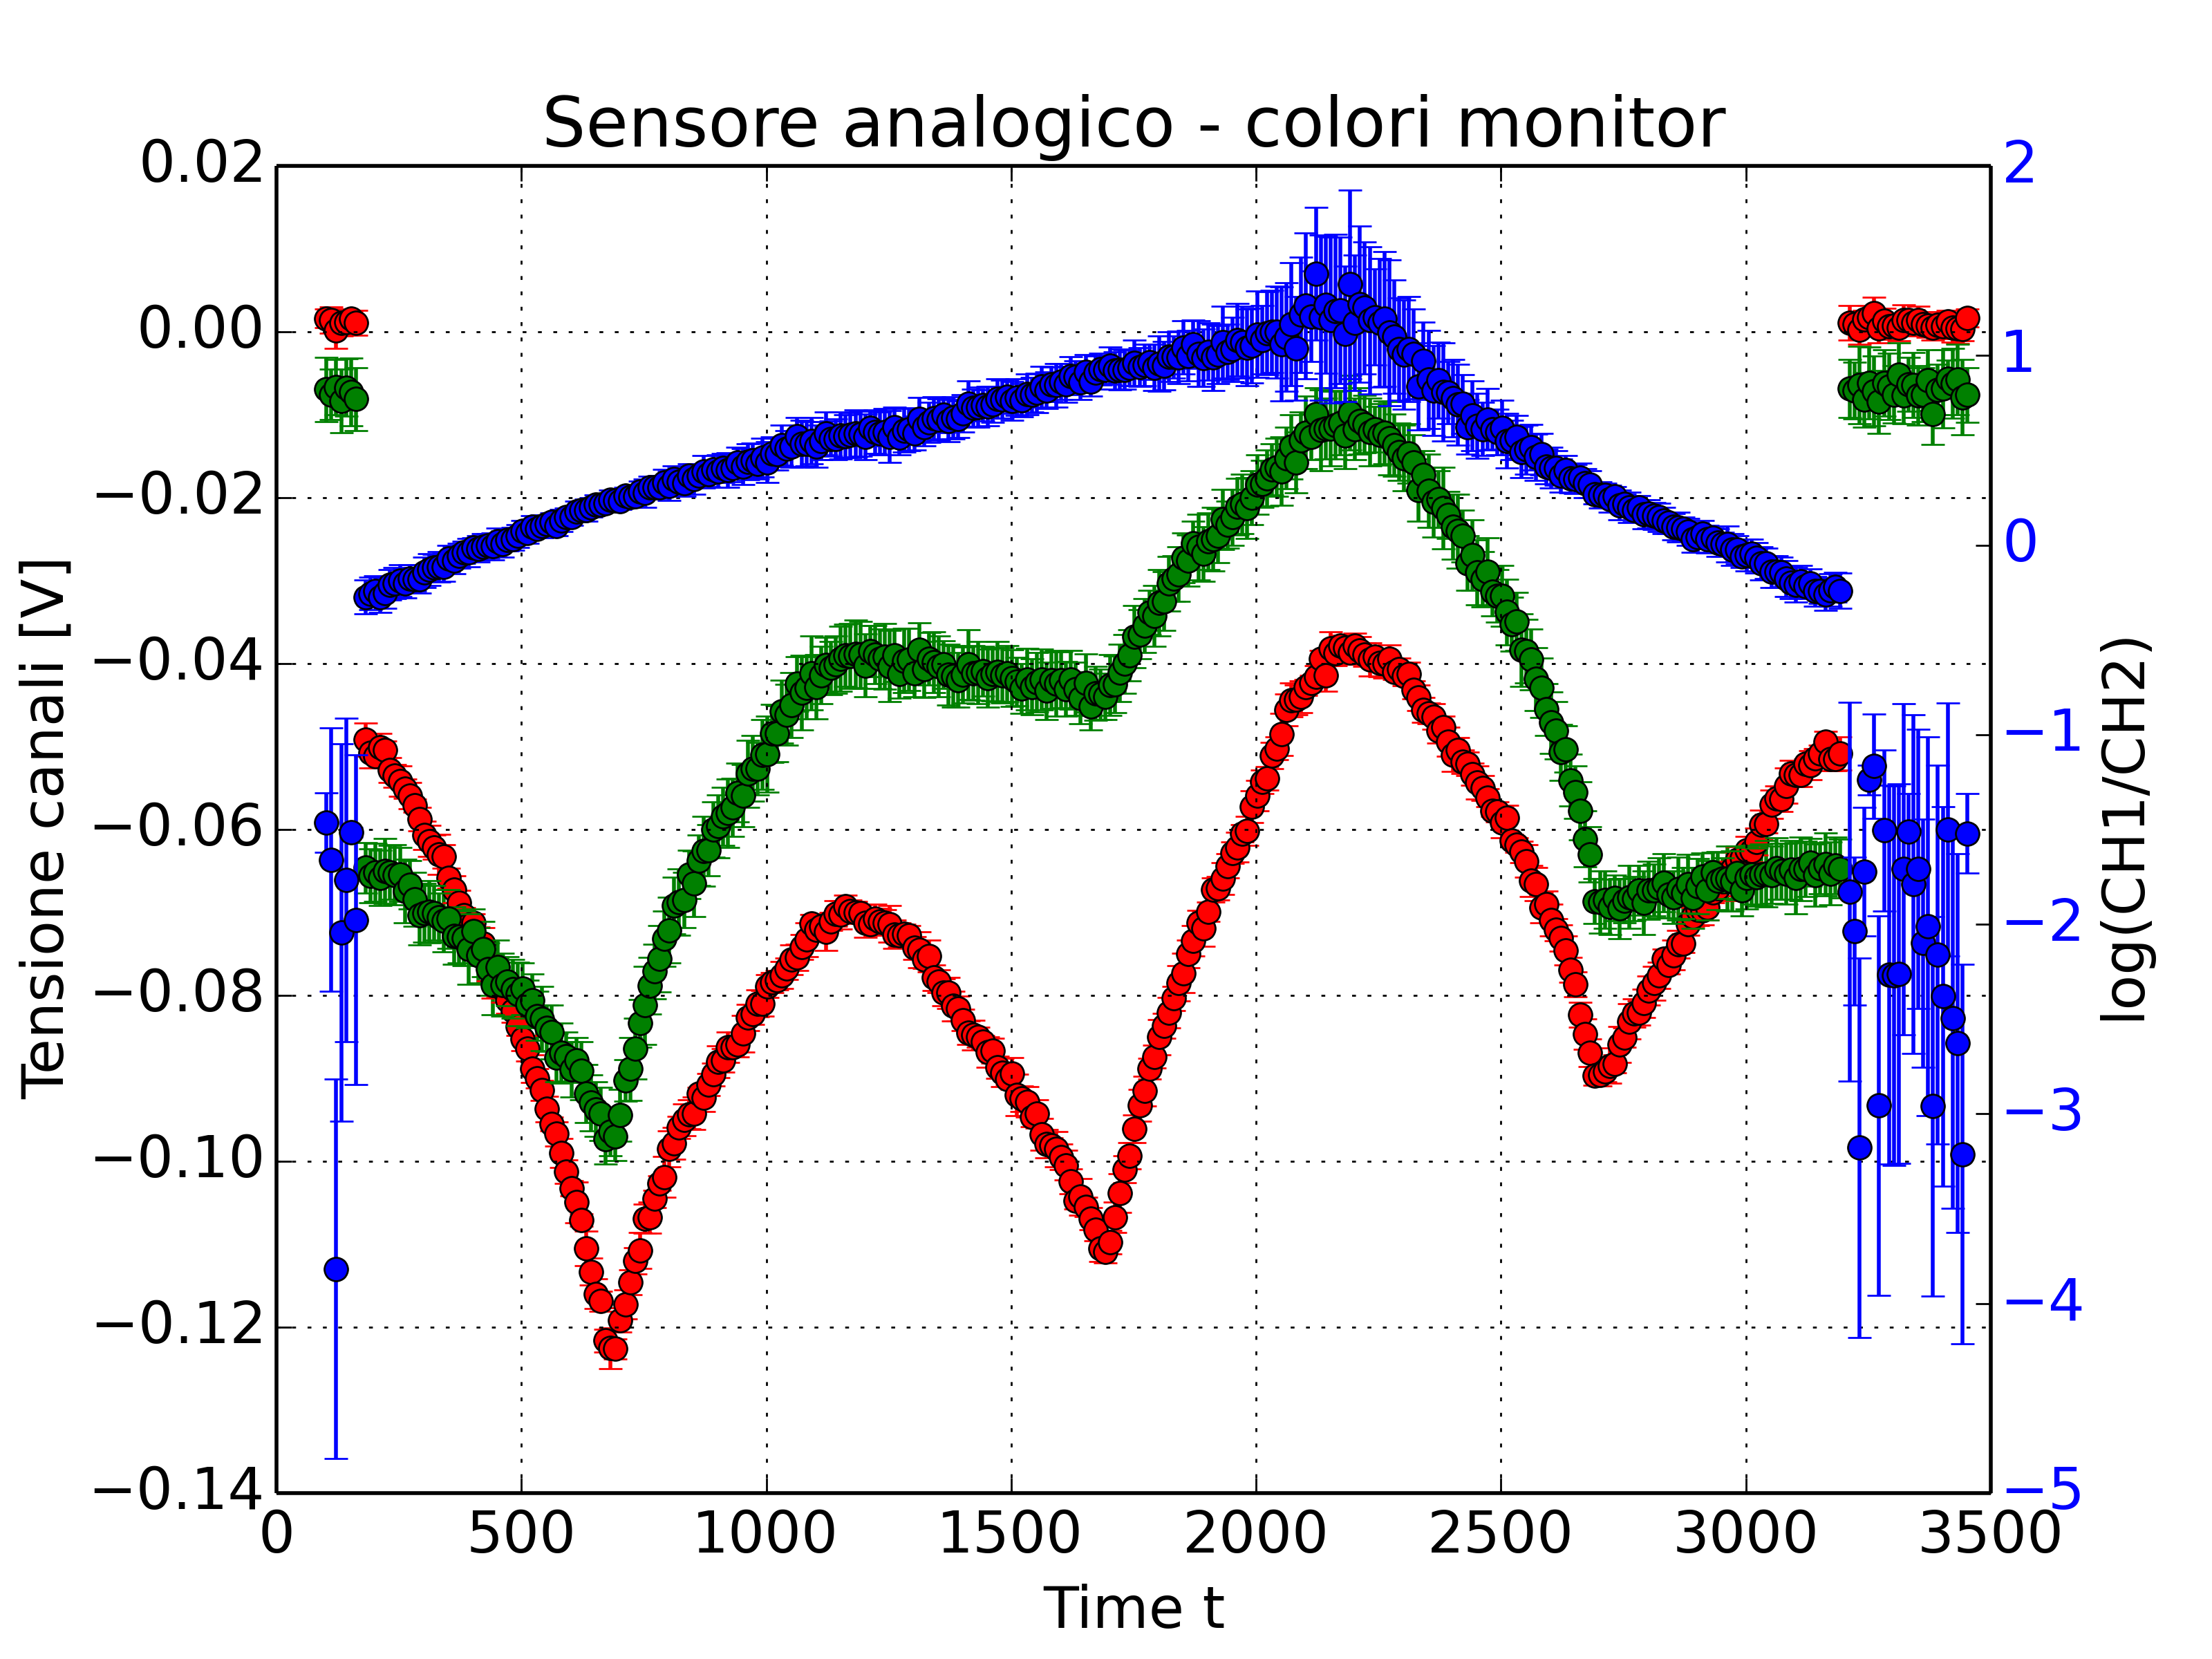
\includegraphics[width=0.7\linewidth]{./analog_segnale_log_average}
\caption{Segnale acquisito dal sensore mediato e ripulito, e logaritmo del rapporto.}
\label{fig:analog_segnale_log_average}
\end{figure}

Per mezzo dello stesso algoritmo usato in precedenza con i LED, sfruttando la curva di calibrazione possiamo stimare la lunghezza d'onda a partire dal log: i valori ottenuti sono provvisti di barra di errore, dato da quello calcolato sul $log(CH1/CH2)$ e si possono vedere in Figura (\ref{fig:monitor_stima_lunghezzaonda}), dove la scala di destra, questa volta, è usata per la \textit{wavelength}. Nella Tabella (\ref{RGB_lambda}) vengono riassunte le $\lambda$ stimate con questo metodo per i colori \textit{puri} RED, GREEN, BLUE. Per riferimento, sono riportati gli intervalli in nm in cui vengono definiti i colori: i dati sono tratti da Wikipedia che a sua volta cita come referenza \cite[Thomas J. Bruno, Paris D. N. Svoronos. CRC Handbook of Fundamental Spectroscopic Correlation Charts]{bib3}. Notiamo che il rosso riusciamo a stimarlo piuttosto bene, il verde inizia ad essere tendente al giallo, invece il blu è accettabile solo entro i limiti dell'errore. Si ricordi che comunque il limite inferiore che possiamo quantificare è dato dalla scala di calibrazione, che termina a 500nm.\\

\begin{table}[h]
\centering
\begin{tabular}{c|c|c|c}
  & \textbf{RED} & \textbf{GREEN} & \textbf{BLUE} \\ 
 \hline Wavelength (nm) & 632(17) & 552(18) & 503(20) \\
 Colour ranges (nm) & 620-750 & 495-570 & 450-495 \\ 
\hline 
\end{tabular} 
\caption{Lunghezza d'onda dei colori puri RGB}
\label{RGB_lambda}
\end{table}

\begin{figure}
\centering
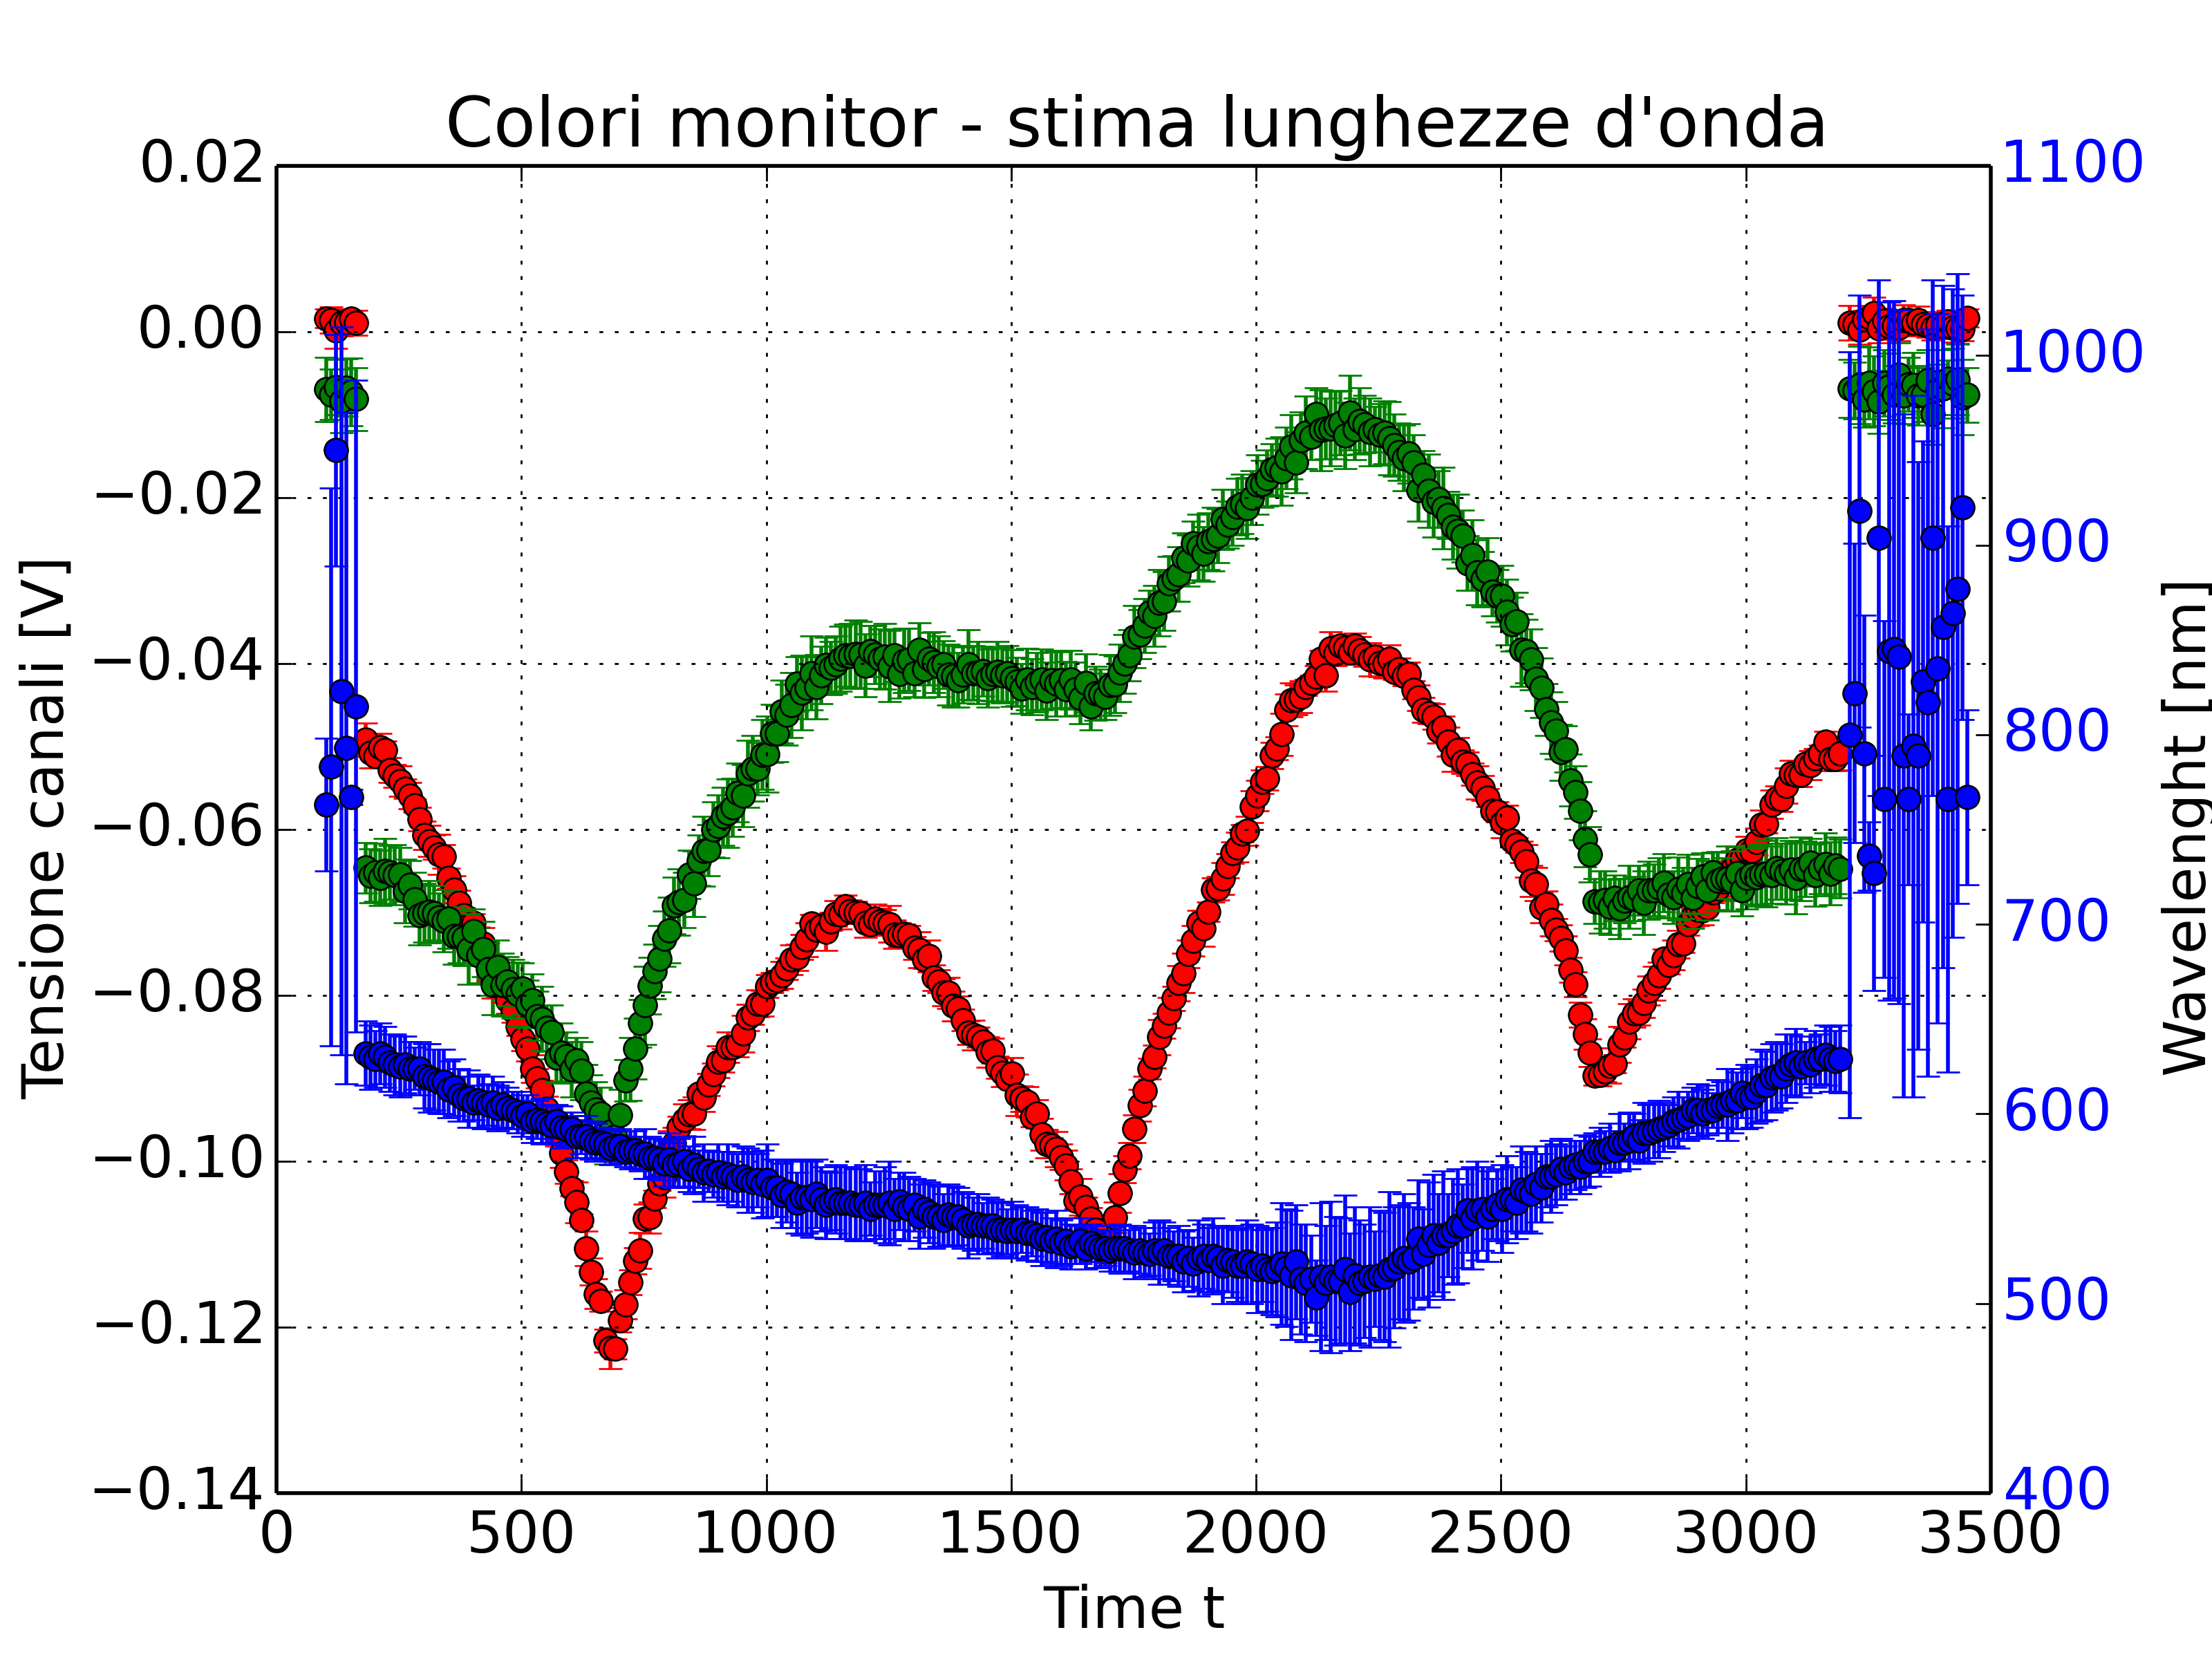
\includegraphics[width=0.7\linewidth]{./monitor_stima_lunghezzaonda}
\caption{Stima della lunghezza d'onda a partire dal logaritmo del rapporto dei segnali, per ogni colore visualizzato sullo schermo.}
\label{fig:monitor_stima_lunghezzaonda}
\end{figure}

Una particolarità che osserviamo anche in questo caso (cfr. sensore digitale) è la presenza di un segnale non nullo in corrispondenza del colore nero proiettato sul monitor LCD. Questa volta il fenomeno è maggiormente evidente poichè è asimmetrico rispetto ai due fotodiodi: il diodo corrispondente al CH2, con curva di responsività piccata sul rosso (nei plot precedenti è la curva verde), rileva un segnale non trascurabile, contrariamente al diodo del CH1 che mostra tensioni compatibili con lo zero. Per essere più precisi: bisogna ricordarsi che esiste un segnale di buio stimato intorno ai 7-8mV che in questo caso incide in misura evidente ma il suo effetto si compensa con quella radiazione di calore infrarossa che viene emanata dal monitor e comunque rilevata dal sensore. In particolare, nel caso del CH1 questi due contributi si annullano a vicenda (uno è negativo e il secondo positivo), mentre nel CH2 prevale l'effetto dell'IR (come ci aspettiamo in base alla responsività spettrale). Si può provare a sottrarre questo fondo IR dal CH2 (il CH1 lo lasciamo inalterato) per vedere se otteniamo delle lunghezze d'onda maggiormente compatibili con i valori di riferimento. \\
Il plot è in Figura (\ref{fig:monitor_stima_lunghezzaonda_senzaIR}): si noti la saturazione a 500nm in corrispondenza del BLU. La stessa tabella di prima può essere riscritta come:

\begin{table}[h]
\centering
\begin{tabular}{c|c|c|c}
  & \textbf{RED} & \textbf{GREEN} & \textbf{BLUE} \\ 
 \hline Wavelength (nm) & 627(18) & 538(15) & $<$500(20) \\
 Colour ranges (nm) & 620-750 & 495-570 & 450-495 \\ 
\hline 
\end{tabular} 
\caption{Lunghezza d'onda dei colori puri RGB - no IR}
\label{RGB_lambda_noIR}
\end{table}
~\\

Il rosso è rimasto più o meno fisso, mentre per il verde abbiamo una corrispondenza molto migliore e quasi coincidente con un verde \textit{puro}. Per quanto riguarda il BLU possiamo agire nel seguente modo: per mezzo di Octave cerchiamo un polinomio interpolatore dei punti di calibrazione e prolunghiamolo per lunghezze d'onda comprese nel range 450-500nm.\\

 
\begin{figure}
\centering
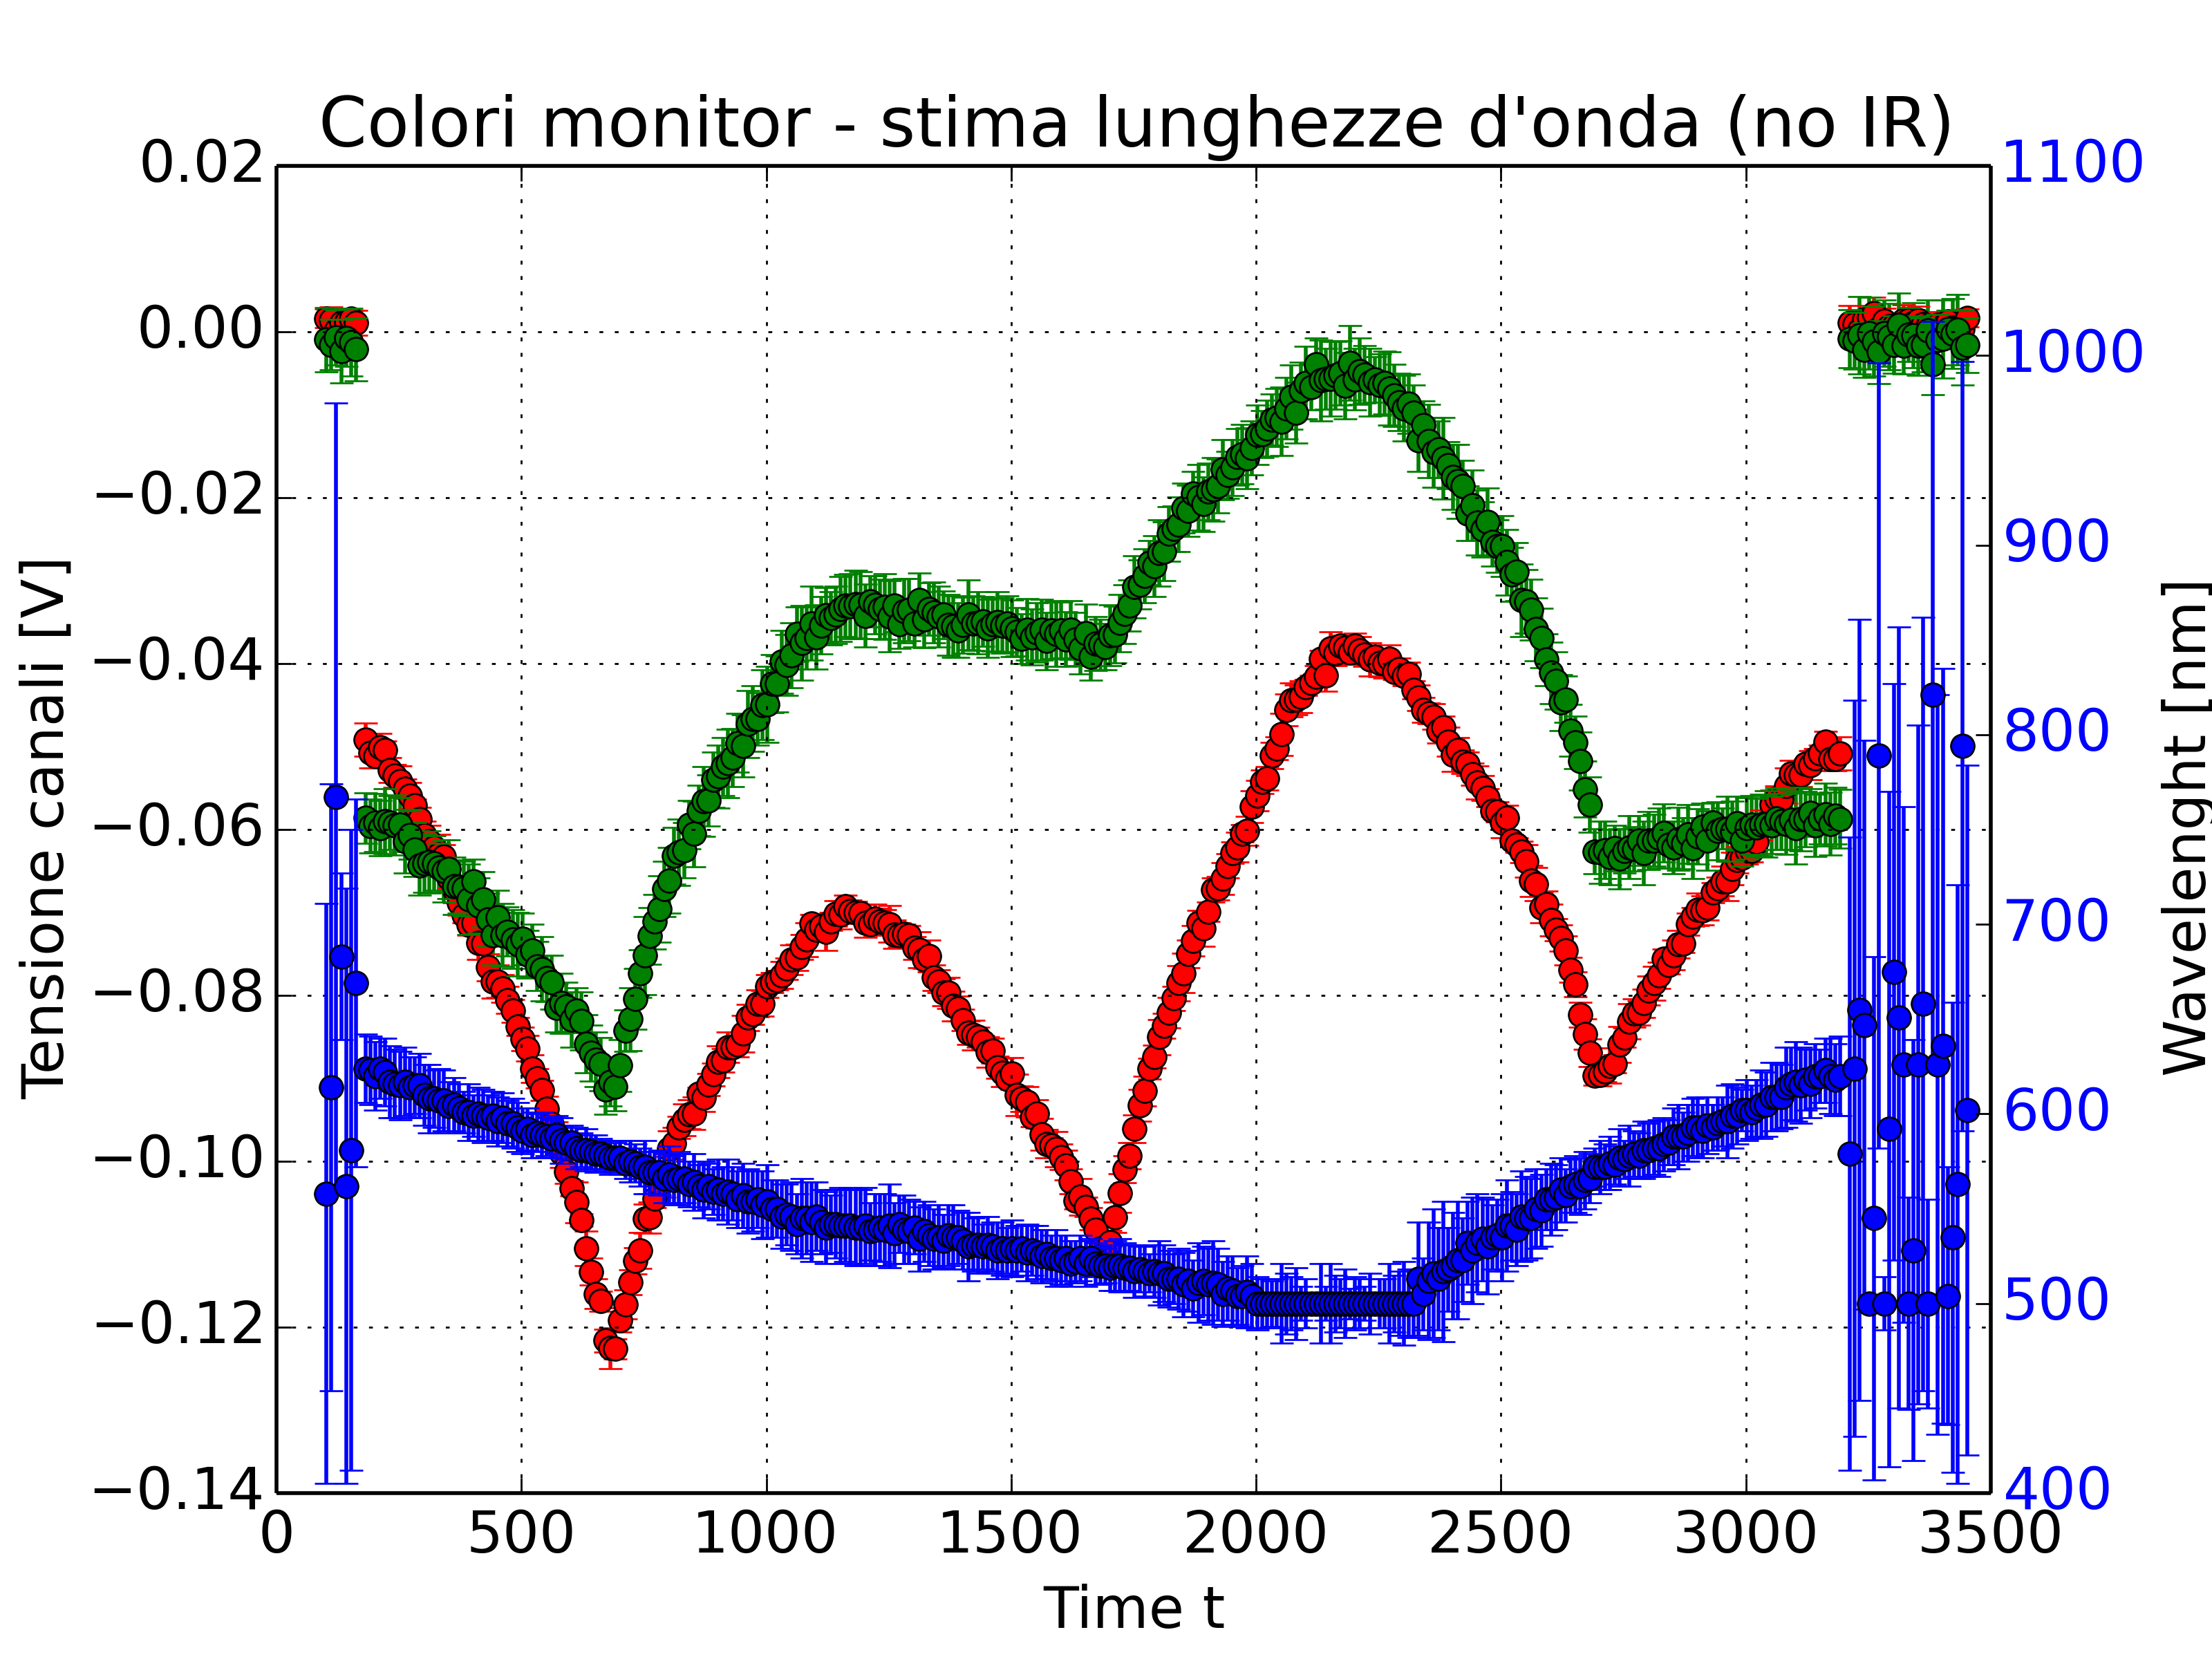
\includegraphics[width=0.7\linewidth]{./monitor_stima_lunghezzaonda_senzaIR}
\caption{Stima della lunghezza d'onda a partire dal logaritmo del rapporto dei segnali, per ogni colore visualizzato sullo schermo, senza IR}
\label{fig:monitor_stima_lunghezzaonda_senzaIR}
\end{figure}


Una certa arbitrarietà sorge nella scelta del grado del polinomio di interpolazione che può condurre ad esiti totalmente differenti fra loro, come una divergenza a $+ \infty$ o a $- \infty$ al diminuire di $\lambda$. Tuttavia possiamo in qualche modo aiutarci modellizzando le curve di responsività come due gaussiane centrate attorno al loro valore massimo (chiaramente esplicitato nel datasheet e riportato nella tabella riassuntiva di inizio capitolo), con larghezza stimabile a partire dal Grafico (\ref{fig:spectral_respo}). Questa modellizzazione è riportata in Figura (\ref{modell+resp}) assieme alla curva originaria per un confronto. Se guardiamo la Figura (\ref{fig:calibrazione_analog}) dove è plottata la curva di calibrazione del sensore analogico per compararla quella del modello gaussiano notiamo ovviamente delle differenze, in particolare nella sua concavità, dovute essenzialmente al fatto che verso le code degli spettri l'approssimazione gaussiana è sempre meno rispettata: si noti, ad esempio, il comportamento del segnale del CH1 per lunghezze d'onda decrescenti. In ogni caso è utile per selezionare il migliore polinomio di interpolazione, scelto di grado 11. La curva di calibrazione \textit{estesa} è in Figura (\ref{fig:calibrazione_ext}) e le lunghezze d'onda estrapolate da questa sono in Figura (\ref{fig:monitor_stima_lunghezzaonda_senzaIR_extended}). \\

\begin{figure}
\centering
\subfloat[Subfigure 1 list of figures text][Modellizzazione della curva di responsività: la curva in rosso rappresenta il logaritmo naturale del rapporto. Per due gaussiane il risultato è una parabola se le loro larghezze sono differenti, altrimenti una retta.]{
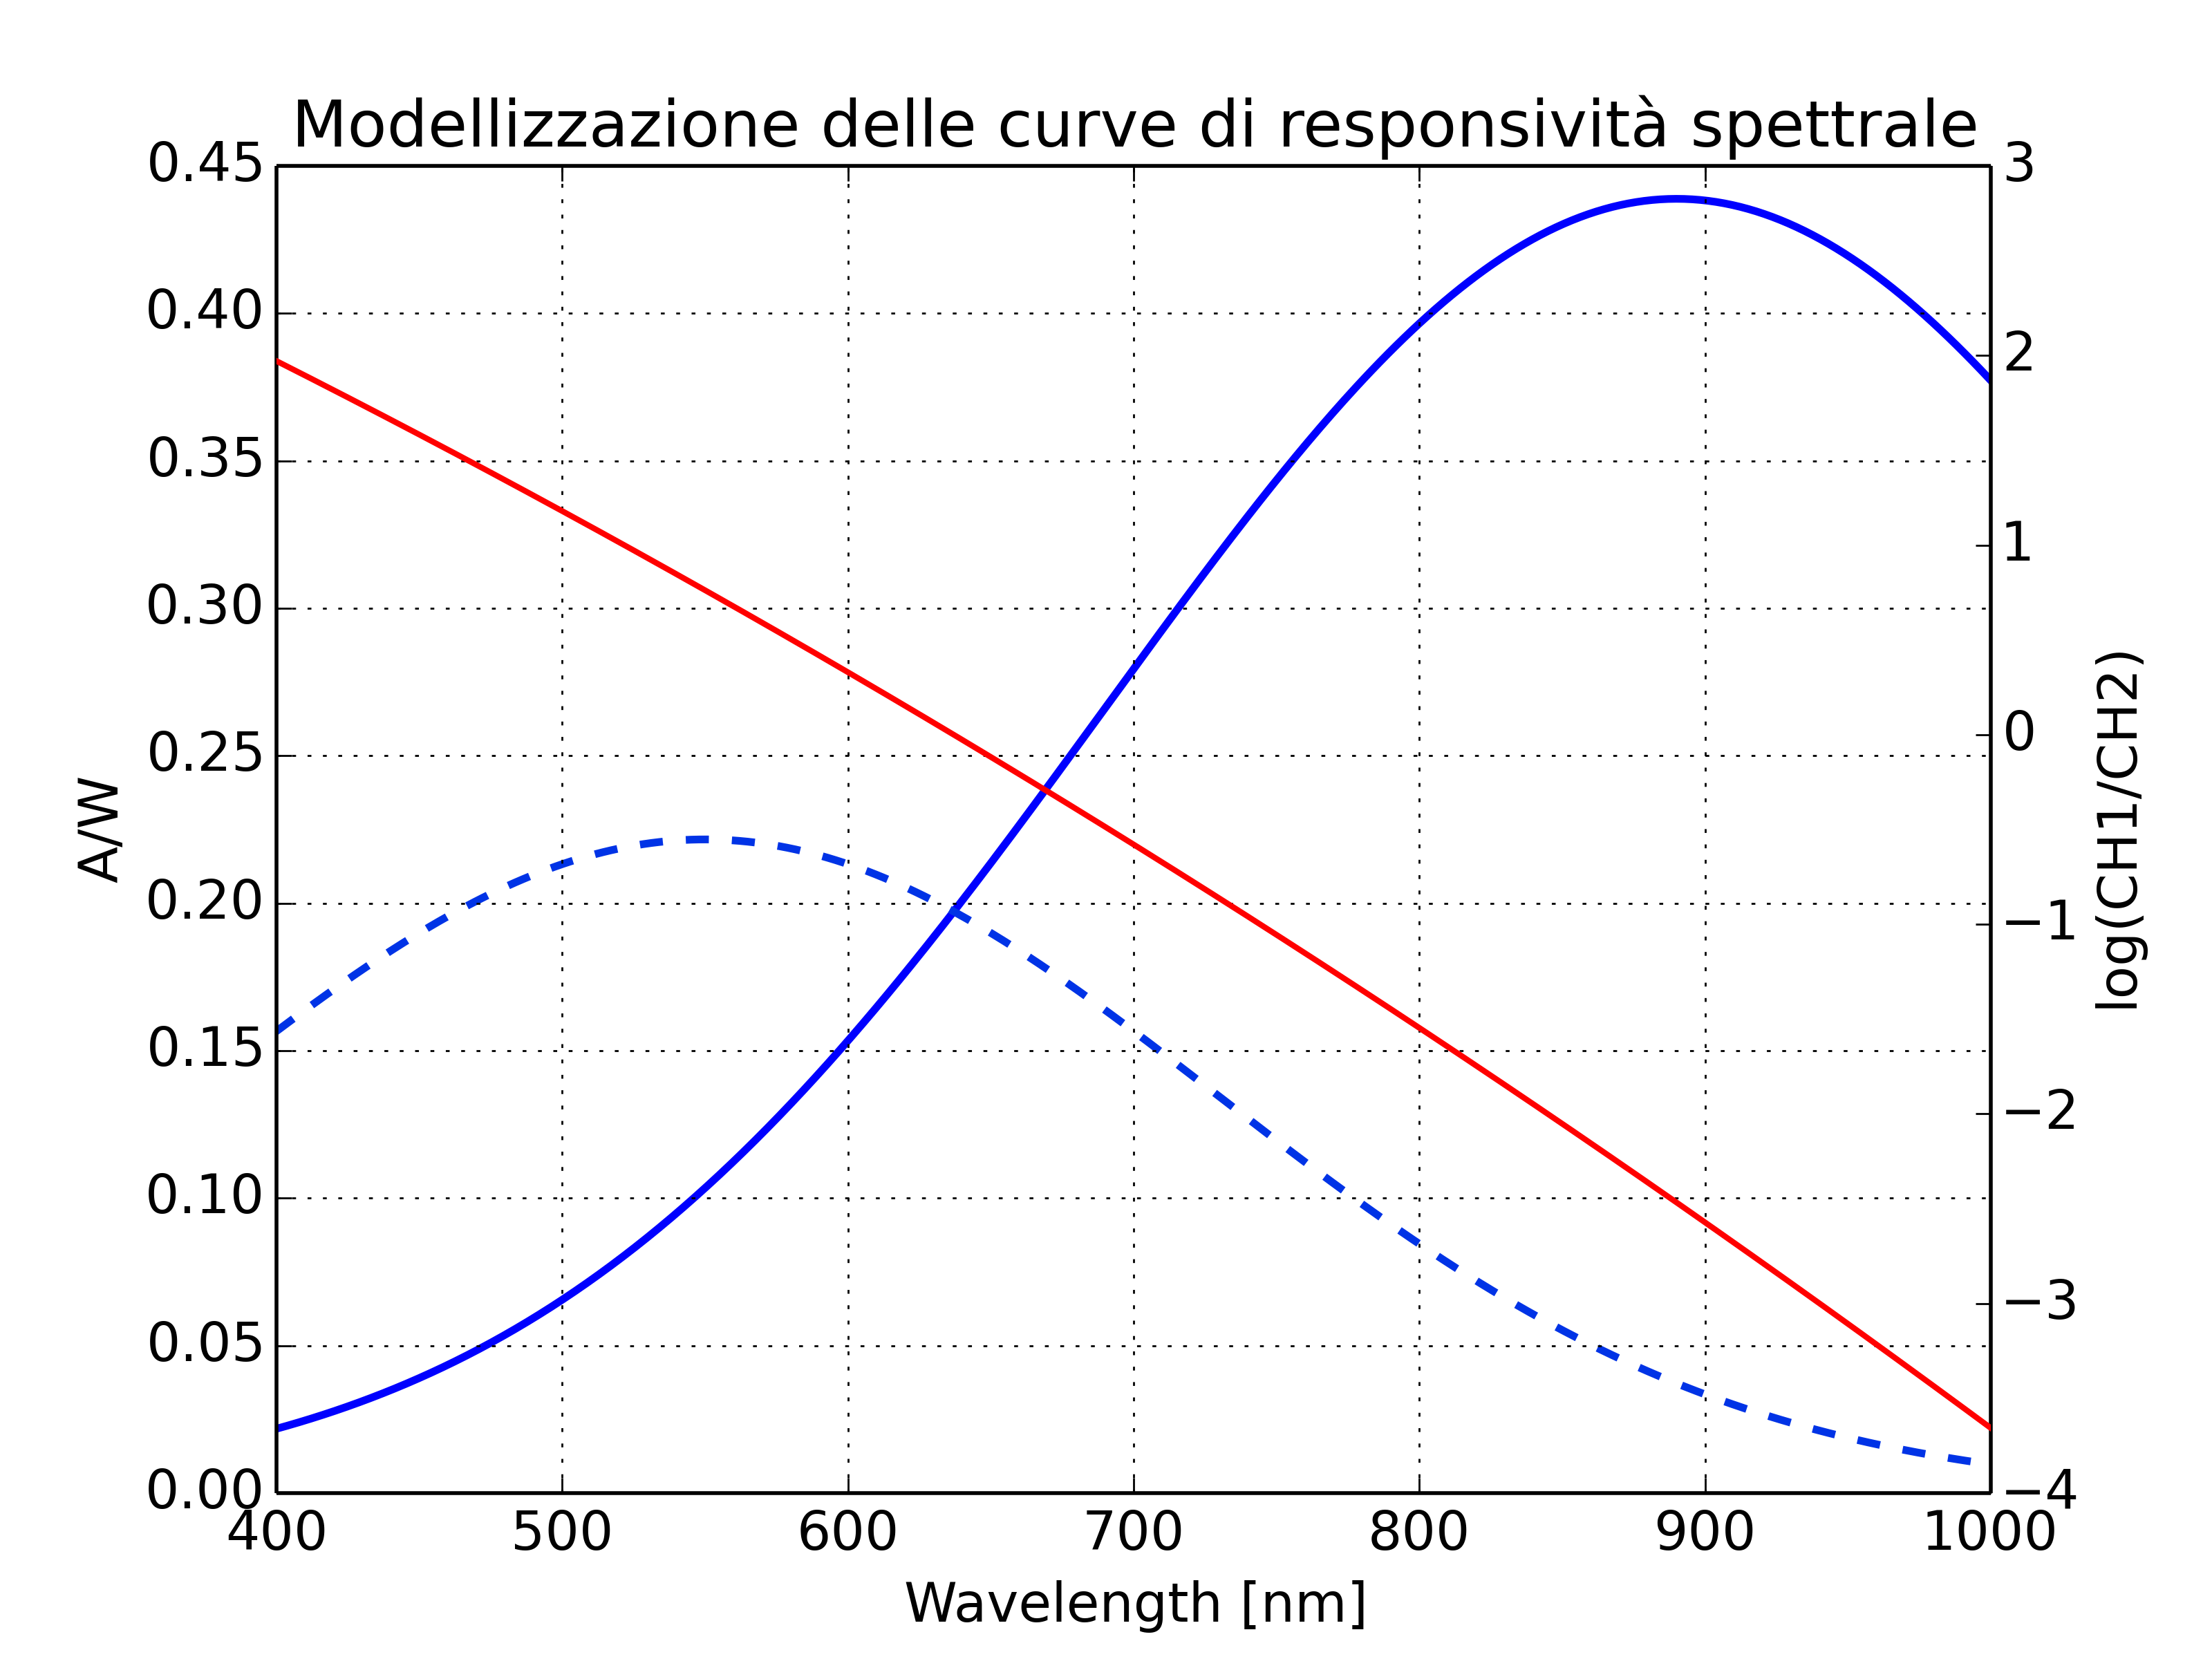
\includegraphics[width=0.6\linewidth]{./normal_respons}
\label{fig:normal_respons}}
%\qquad
\subfloat[Subfigure 2 list of figures text][Curva di responsività spettrale dei due diodi in funzione della lunghezza d'onda incidente.]{
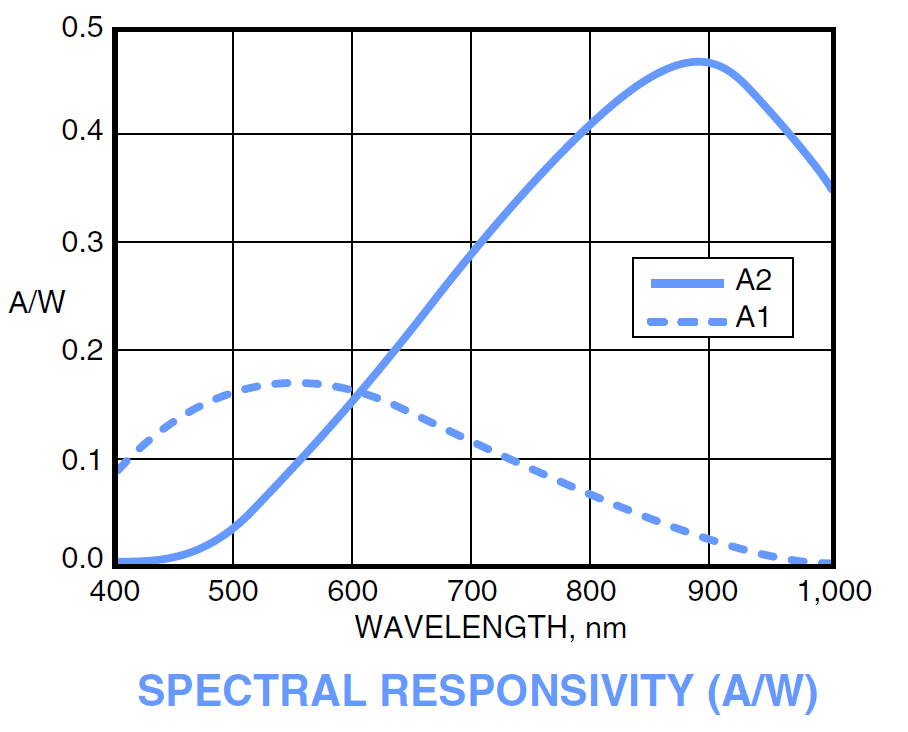
\includegraphics[width=0.6\linewidth]{./spectral_respo}
\label{fig:spectral_respo1}}
%\qquad

\caption{}
\label{modell+resp}
\end{figure}


\begin{figure}
\centering
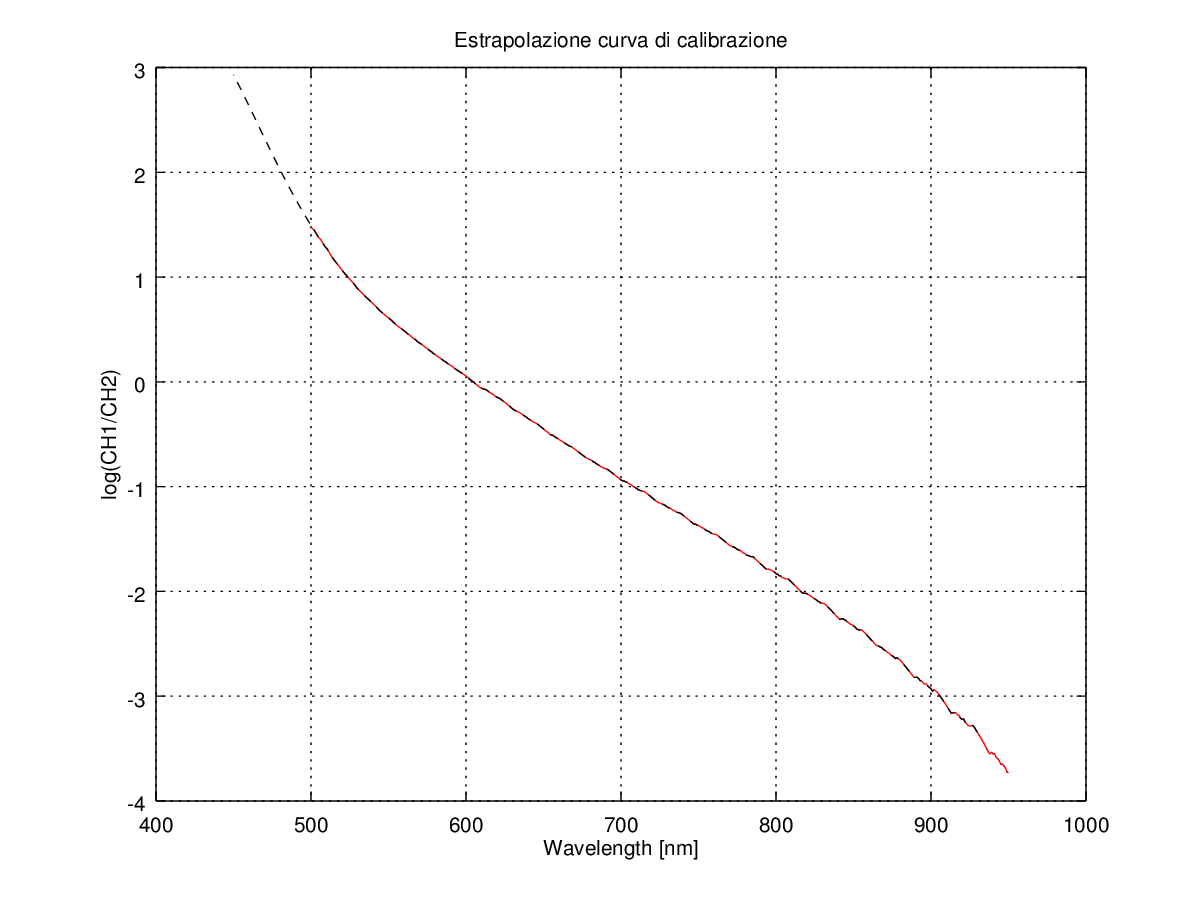
\includegraphics[width=0.7\linewidth]{./calibrazione_ext}
\caption{Curva di calibrazione "estesa" interpolata con un polinomio di grado 11.}
\label{fig:calibrazione_ext}
\end{figure}

\begin{figure}
\centering
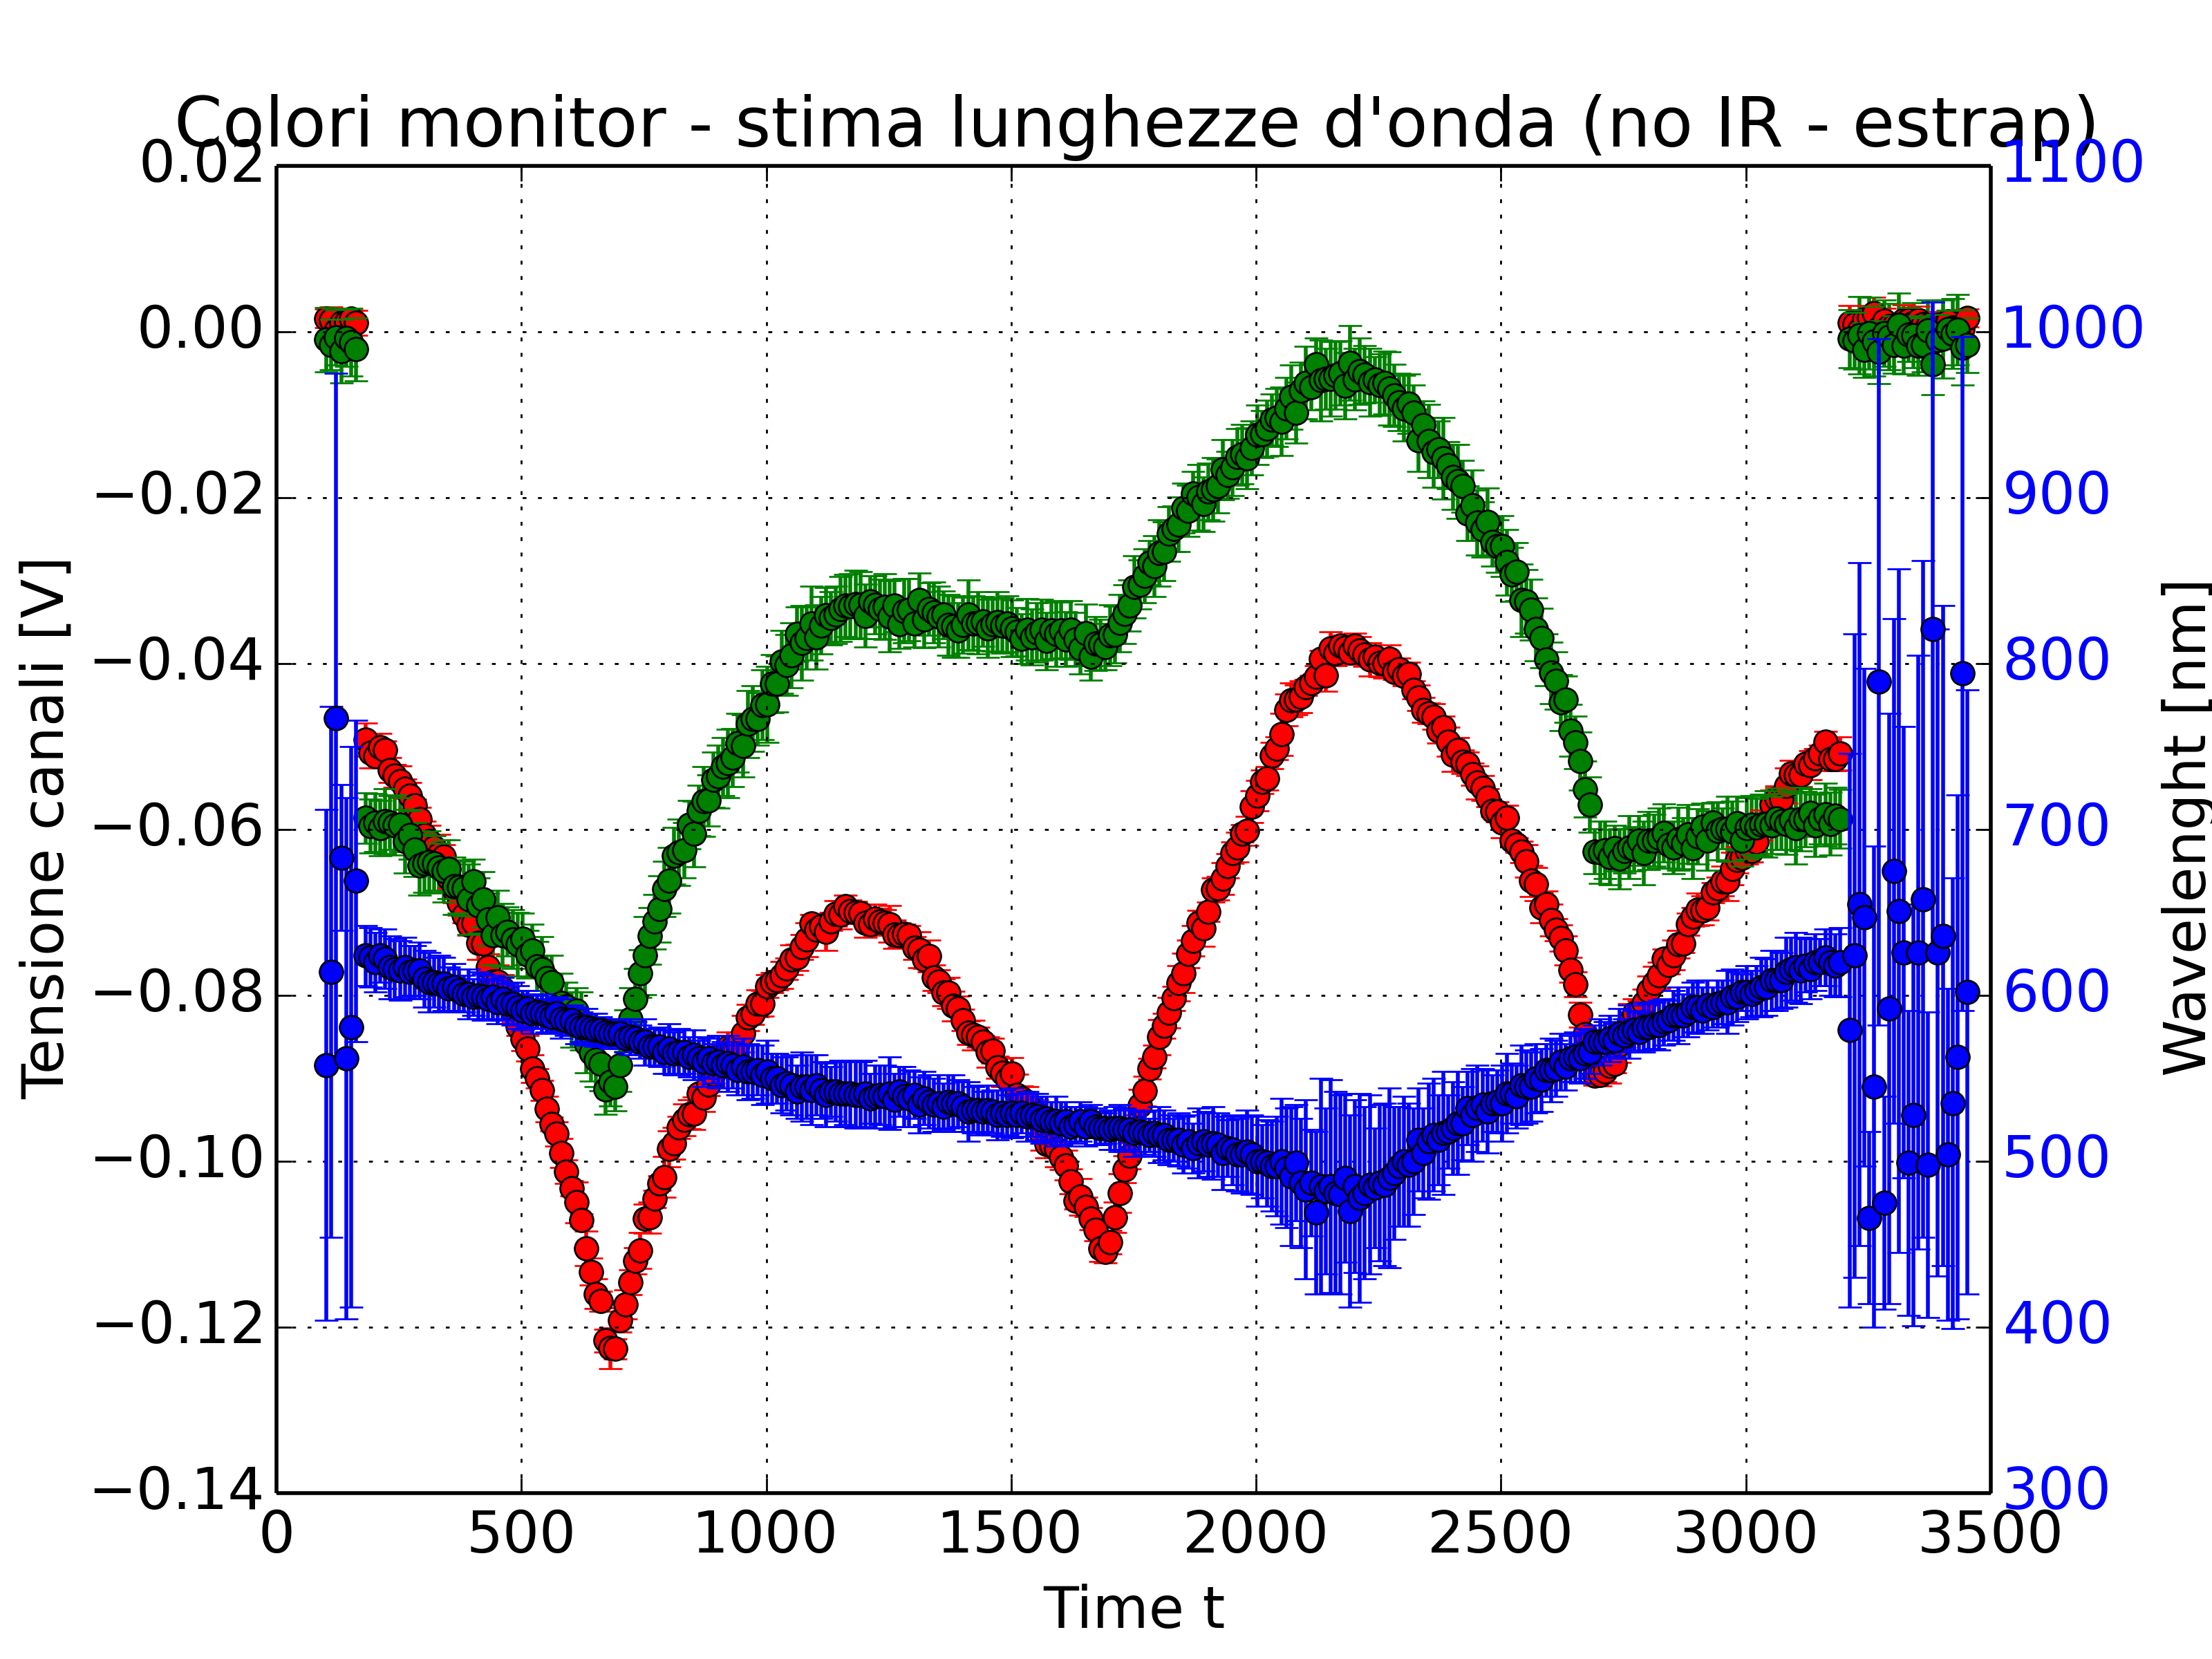
\includegraphics[width=0.7\linewidth]{./monitor_stima_lunghezzaonda_senzaIR_extended}
\caption{Stima della lunghezza d'onda del monitor: senza fondo IR ed usando la curva di calibrazione "estesa".}
\label{fig:monitor_stima_lunghezzaonda_senzaIR_extended}
\end{figure}

I risultati delle $\lambda$ per i colori puri sono riassunti in Tabella (\ref{RGB_lambda_noIR_ext}): il rosso e il verde sono (ovviamente) rimasti gli stessi, in buon accordo con le lunghezze d'onda effettive; finalmente il blu, nonostante un errore considerevole dovuto essenzialmente alla bassissima responsività del fotodiodo 2 a lunghezze d'onda fra 400-500 nm, e quindi con un errore percentuale affatto trascurabile, risulta avere una $\lambda$ decisamente buona, circa a metà dell'intervallo di definizione.\\

\begin{table}[h]
\centering
\begin{tabular}{c|c|c|c}
  & \textbf{RED} & \textbf{GREEN} & \textbf{BLUE} \\ 
 \hline Wavelength (nm) & 627(18) & 538(15) & 470(50) \\
 Colour ranges (nm) & 620-750 & 495-570 & 450-495 \\ 
\hline 
\end{tabular} 
\caption{Lunghezza d'onda dei colori puri RGB - no IR}
\label{RGB_lambda_noIR_ext}
\end{table}
~\\

Per dimostrare in maniera forse più significativa la validità dell'estrapolazione offerta della curva di calibrazione per lunghezze d'onda fra 450-500 nm, ritorniamo al grafico dei LED di Figura (\ref{fig:calibrazione_led}): si ricorda che per i LED nel blu non vi erano punti della curva con cui quantificare l'eventuale scostamento della lunghezza d'onda. Proviamo, quindi, a riplottare esattamente lo stesso grafico usando, questa volta, la curva \textit{estesa} per verificare se la nostra estrapolazione è stata efficace. Il risultato, in Figura (\ref{LED_wavel_ext}) è davvero buono ed offre una giustificazione indipendente del procedimento seguito, da cui segue che anche i valori di $\lambda$ ottenuti per il blu del monitor possiedono una certa significatività.

\begin{figure}
\centering
\subfloat[Subfigure 1 list of figures text][Dispersione dei LED sulla curva di calibrazione 'estesa' del sensore analogico.]{
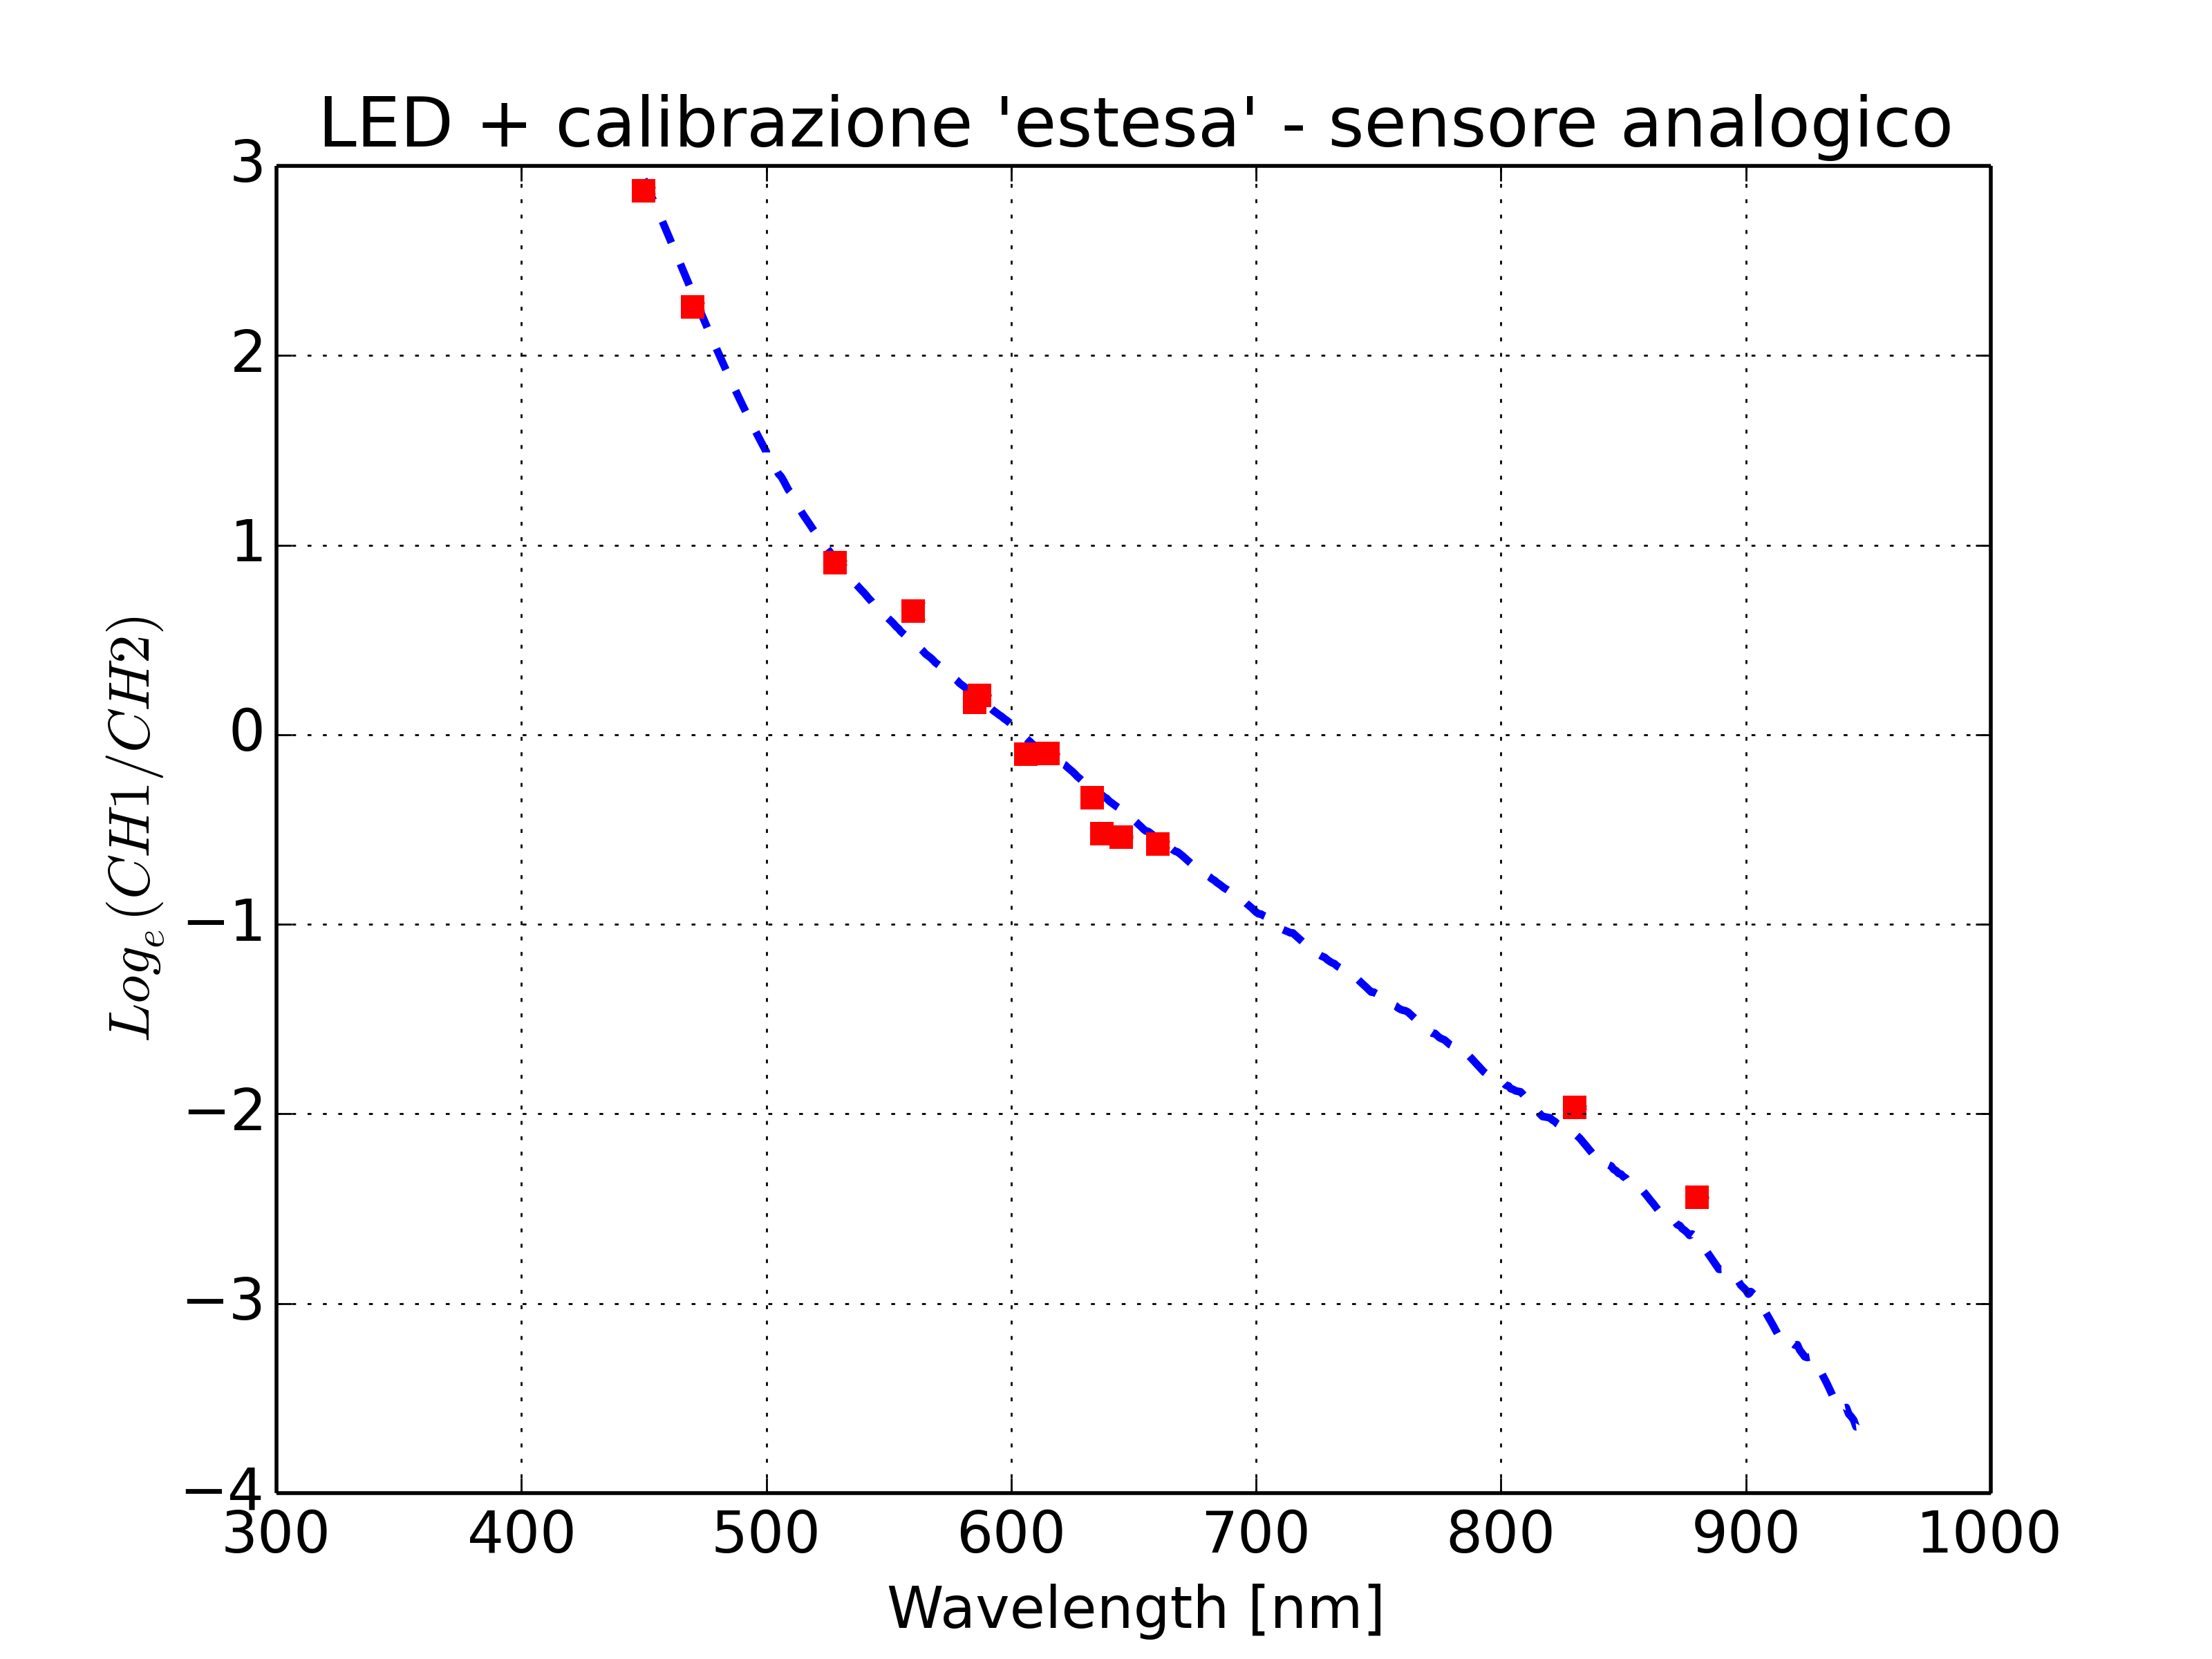
\includegraphics[width=0.6\linewidth]{./calibrazione_LED_extended}
\label{fig:calibrazione_led_extended}}
%\qquad
\subfloat[Subfigure 2 list of figures text][Scarto fra lunghezze d'onda di "fabbrica" e da "calibrazione" per ciascun LED.]{
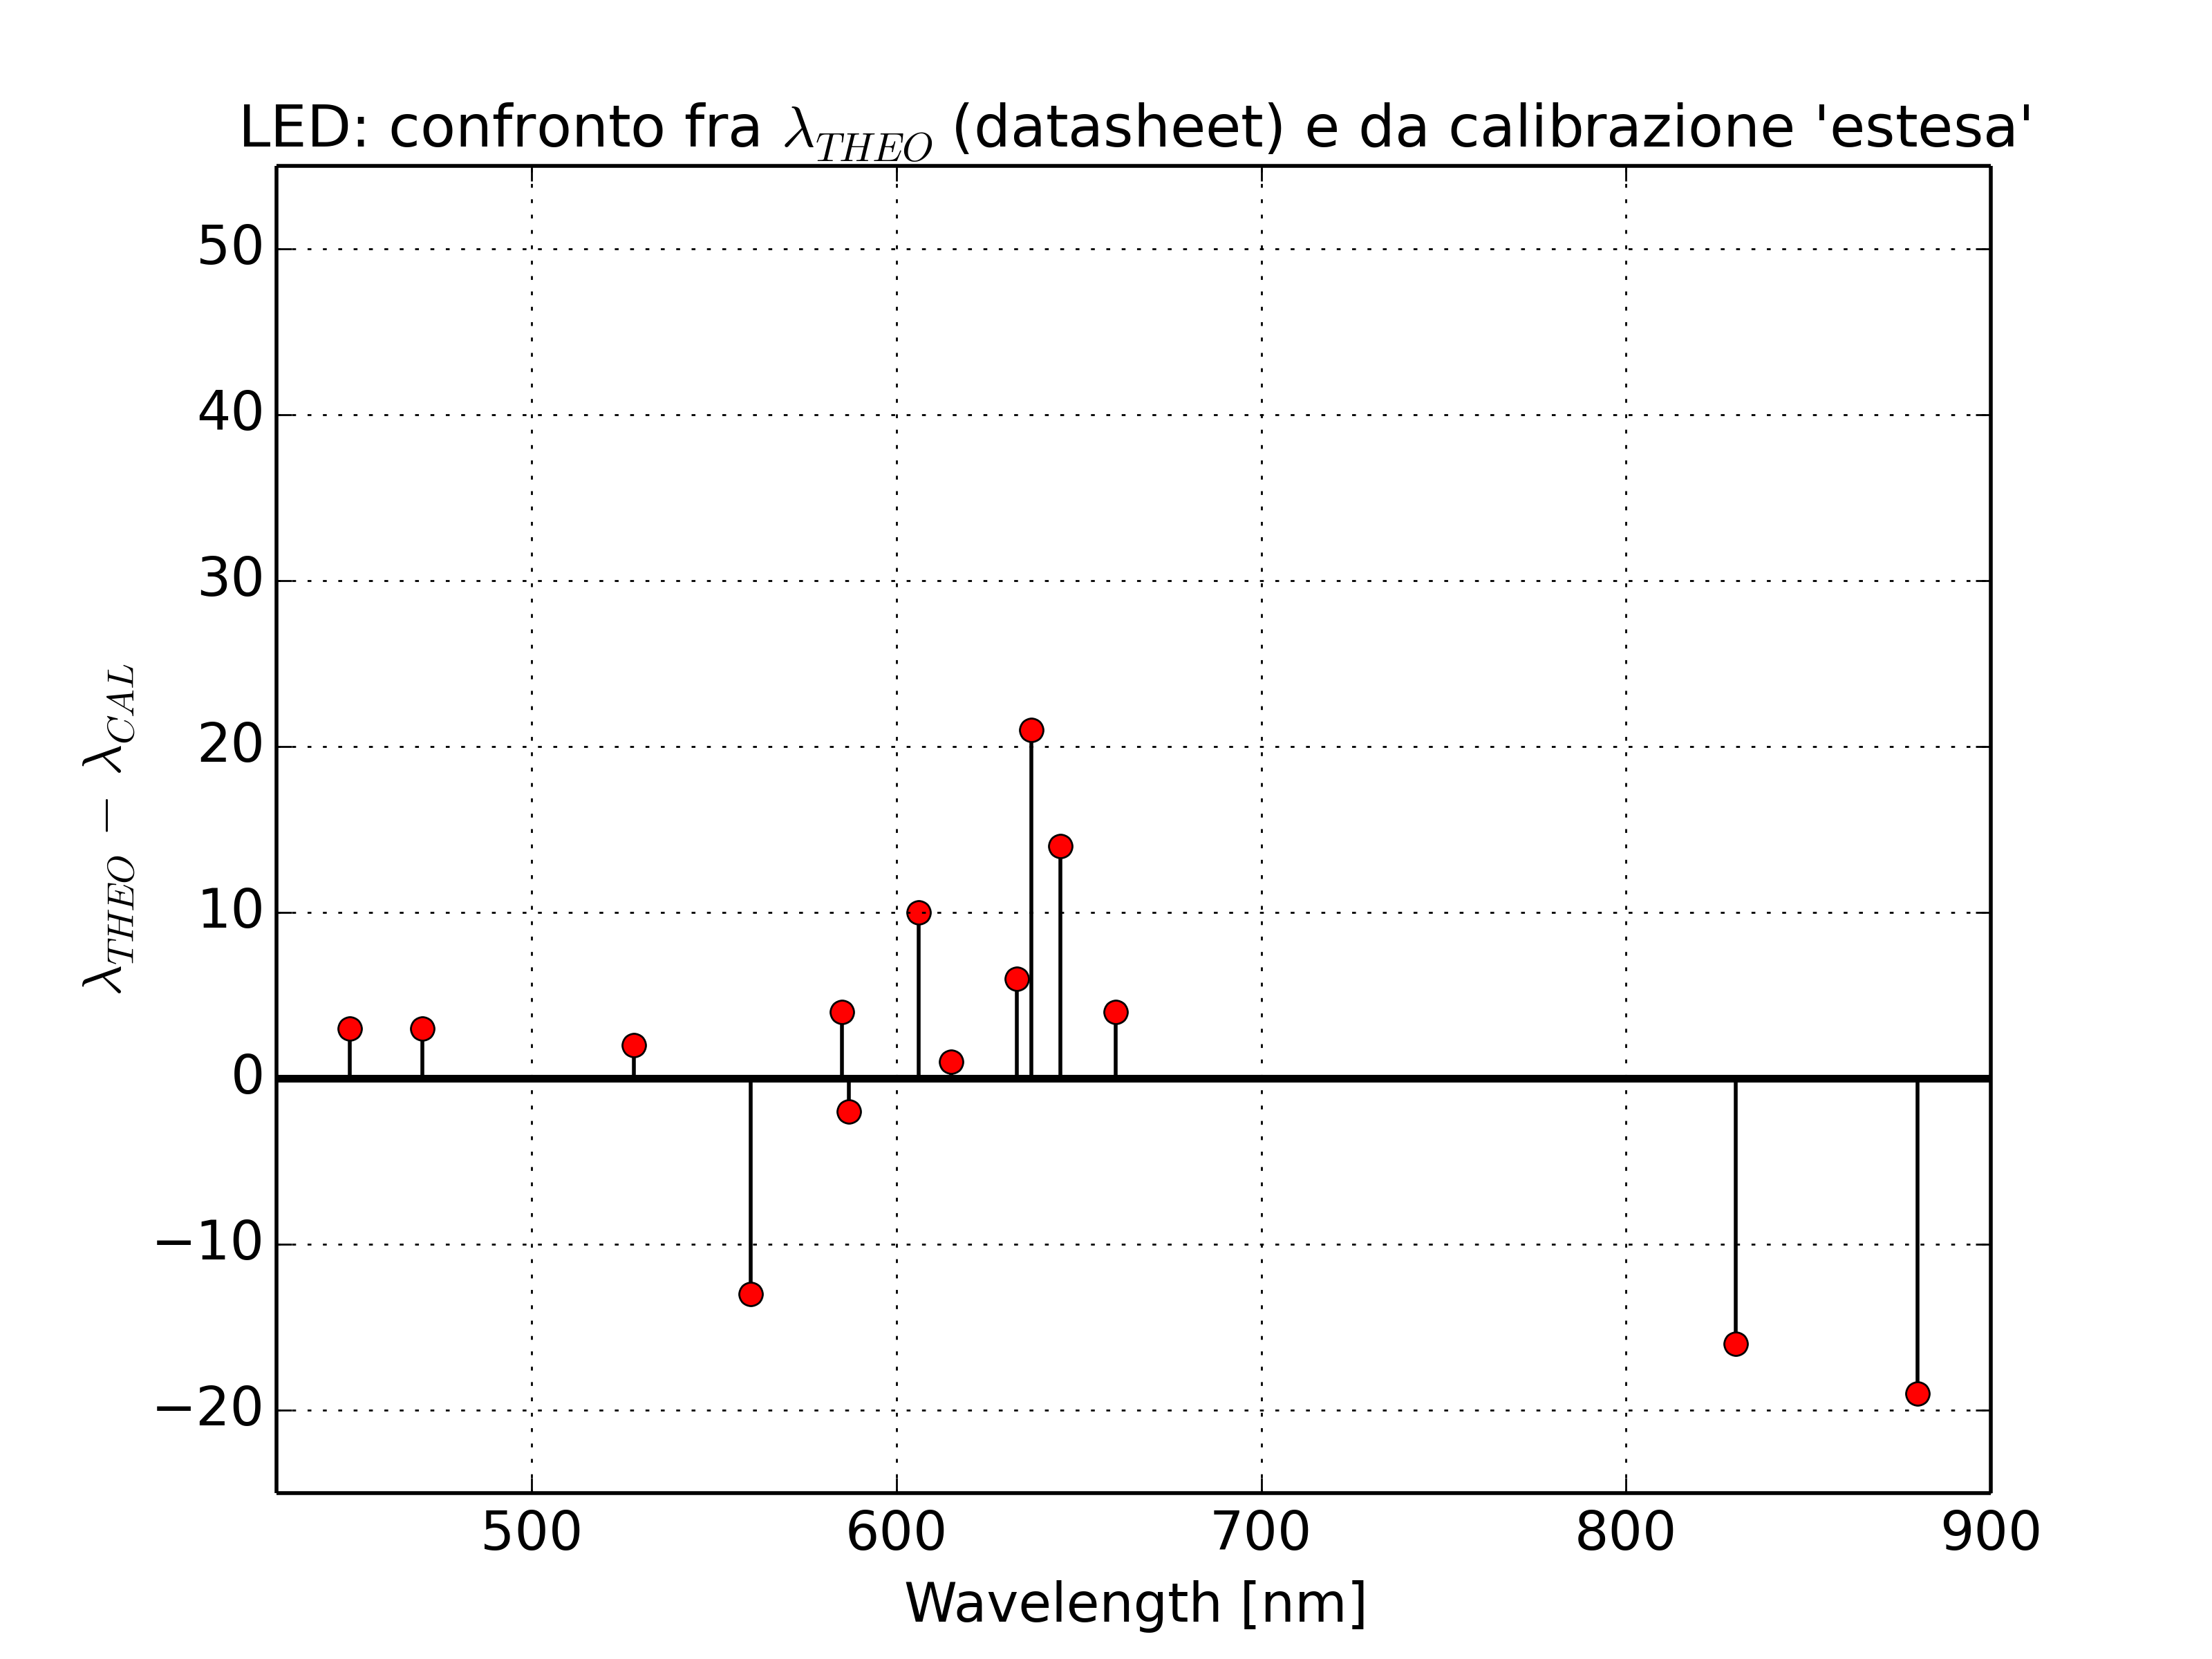
\includegraphics[width=0.6\linewidth]{./LED_confronto_extended}
\label{fig:LED_confronto_extended}}
%\qquad

\caption{Rilevazione della lunghezza d'onda dei LED e confronto con il valore atteso.}
\label{LED_wavel_ext}
\end{figure}

Infine, si riporta una Tabella (\ref{tabella_LED_ext}) riassuntiva con i valori nominali e quelli calcolati per interpolazione della curva di calibrazione "estesa" delle lunghezze d'onda dei LED impiegati.

\begin{table}[h]
\centering
% This LaTeX table template is generated by emacs 24.3.1
\begin{tabular}{l|c|c}
\hline
\textbf{LED} & \textbf{Wavelength} nominal (nm) & \textbf{Wavelength} calibr. (nm) \\
\hline
\textsc{hlmpd101-645} & 645 & 659(1) \\
\textsc{hlmpc115-red} & 637 & 658(2)  \\
\textsc{hlmpc315-Y} & 585 & 589(2)  \\
\textsc{la3366} & 615 & 616(1) \\
\textsc{lb3333} & 470 & 473(1) \\
\textsc{led450} & 450 & 453(1) \\
\textsc{lo3336} & 606 & 616(1) \\
\textsc{lpk376} & 560 & 547(4) \\
\textsc{ls3336} & 633 & 639(1) \\
\textsc{lt3333} & 528 & 530(1) \\
\textsc{ly3336} & 587 & 585(1) \\
\textsc{sfh4873-880} & 880 & 861(1) \\
\textsc{ssl-lxa} & 660 & 664(2) \\
\textsc{tshg8400-830} & 830 & 814(1) \\
\hline
\end{tabular}
\caption{Lunghezze d'onda dei LED ricavate da calibrazione del sensore analogico.}
\label{tabella_LED_ext}
\end{table}
~\\


\subsection{BONUS FINALE: }
In quest'ultima sezione vogliamo presentare un ultimo risultato che si può ottenere con le informazioni acquisite nel corso dell'esperienza della \textsc{week09} unitamente ai dispositivi impiegati in queste settimane: in particolare ci interessa studiare la risposta della fotocellula al silicio alla proiezione dei colori (ottenuti tramite il solito script) sul monitor e legare questi dati alla lunghezza d'onda rilevata dal sensore analogico \textsc{WS-7.56-TO5}. Un aspetto rilevante non secondario consiste in una valutazione indipendente della bontà del modello quadratico che avevamo proposto per spiegare l'andamento della tensione ai capi della fotocellula in funzione delle triplette RGB.\\
Prima di procedere con la discussione, è opportuno riassumere alcuni punti che saranno essenziali nel seguito:

\begin{itemize}
\item La lunghezza d'onda ottenuta per interpolazione della curva di calibrazione ha un senso fisico solo per le situazioni in cui si ha \textit{un solo} led RGB acceso, poichè, ovviamente, la radiazione che incide sul fotorivelatore ha una $\lambda$ definita. Per tutte le altre configurazioni RGB quella che noi chiamiamo lunghezza d'onda in realtà ha un significato completamente diverso e non è facile ipotizzare fin da subito quale questo possa essere. Ad esempio, sia per la configurazione (0.4,1,0) che per (0.8,0,1) viene rilevata una "pseudo" $\lambda$ di circa 550nm: è evidente che queste non possano essere triplette associate allo stesso colore.

\item Nel corso della week09 era stato proposto un modello quadratico dei coefficienti RGB che potesse spiegare la curva di intensità della fotocellula in risposta alle triplette sul monitor. Il modello è come segue:

\begin{equation}
S_{TOT} = a_R^2 S_R + a_B^2 S_B + a_G^2 S_G
\end{equation}

dove $S_R$, $S_B$, $S_G$ corrispondono ai segnali dei colori puri e i coefficienti a sono proprio i componenti della tripletta (R,G,B)=($a_R$, $a_G$, $a_B$). La seguente normalizzazione del modello ci ha permesso di estrarre i rapporti tra le intensità dei colori puri: questi dati sembrano corrispondere qualitativamente alla curva di intensità di una fotocellula calibrata per avere una responsività spettrale simile a quella dell'occhio umano e centrata sul verde.

\begin{equation}
S_{TOT} = \frac{a_R^2 S_R + a_B^2 S_B + a_G^2 S_G}{a_R^2 + a_B^2 + a_G^2}
\end{equation}

\begin{table}
\centering
\begin{tabular}{c|c}
\hline Colore RGB & Intens. relat. (to G) \\ 
\hline GREEN & 1 \\ 
 RED & 0.854 \\ 
 BLUE & 0.663 \\ 
\hline 
\end{tabular} 
\end{table}
~\\

Si riporta in Figura (\ref{modello_quad}) il grafico del modello teorico quadratico (normalizzato e non) con i punti sperimentali acquisiti.

\begin{figure}
\centering
\subfloat[Subfigure 1 list of figures text][Modello quadratico dei coefficienti RGB.]{
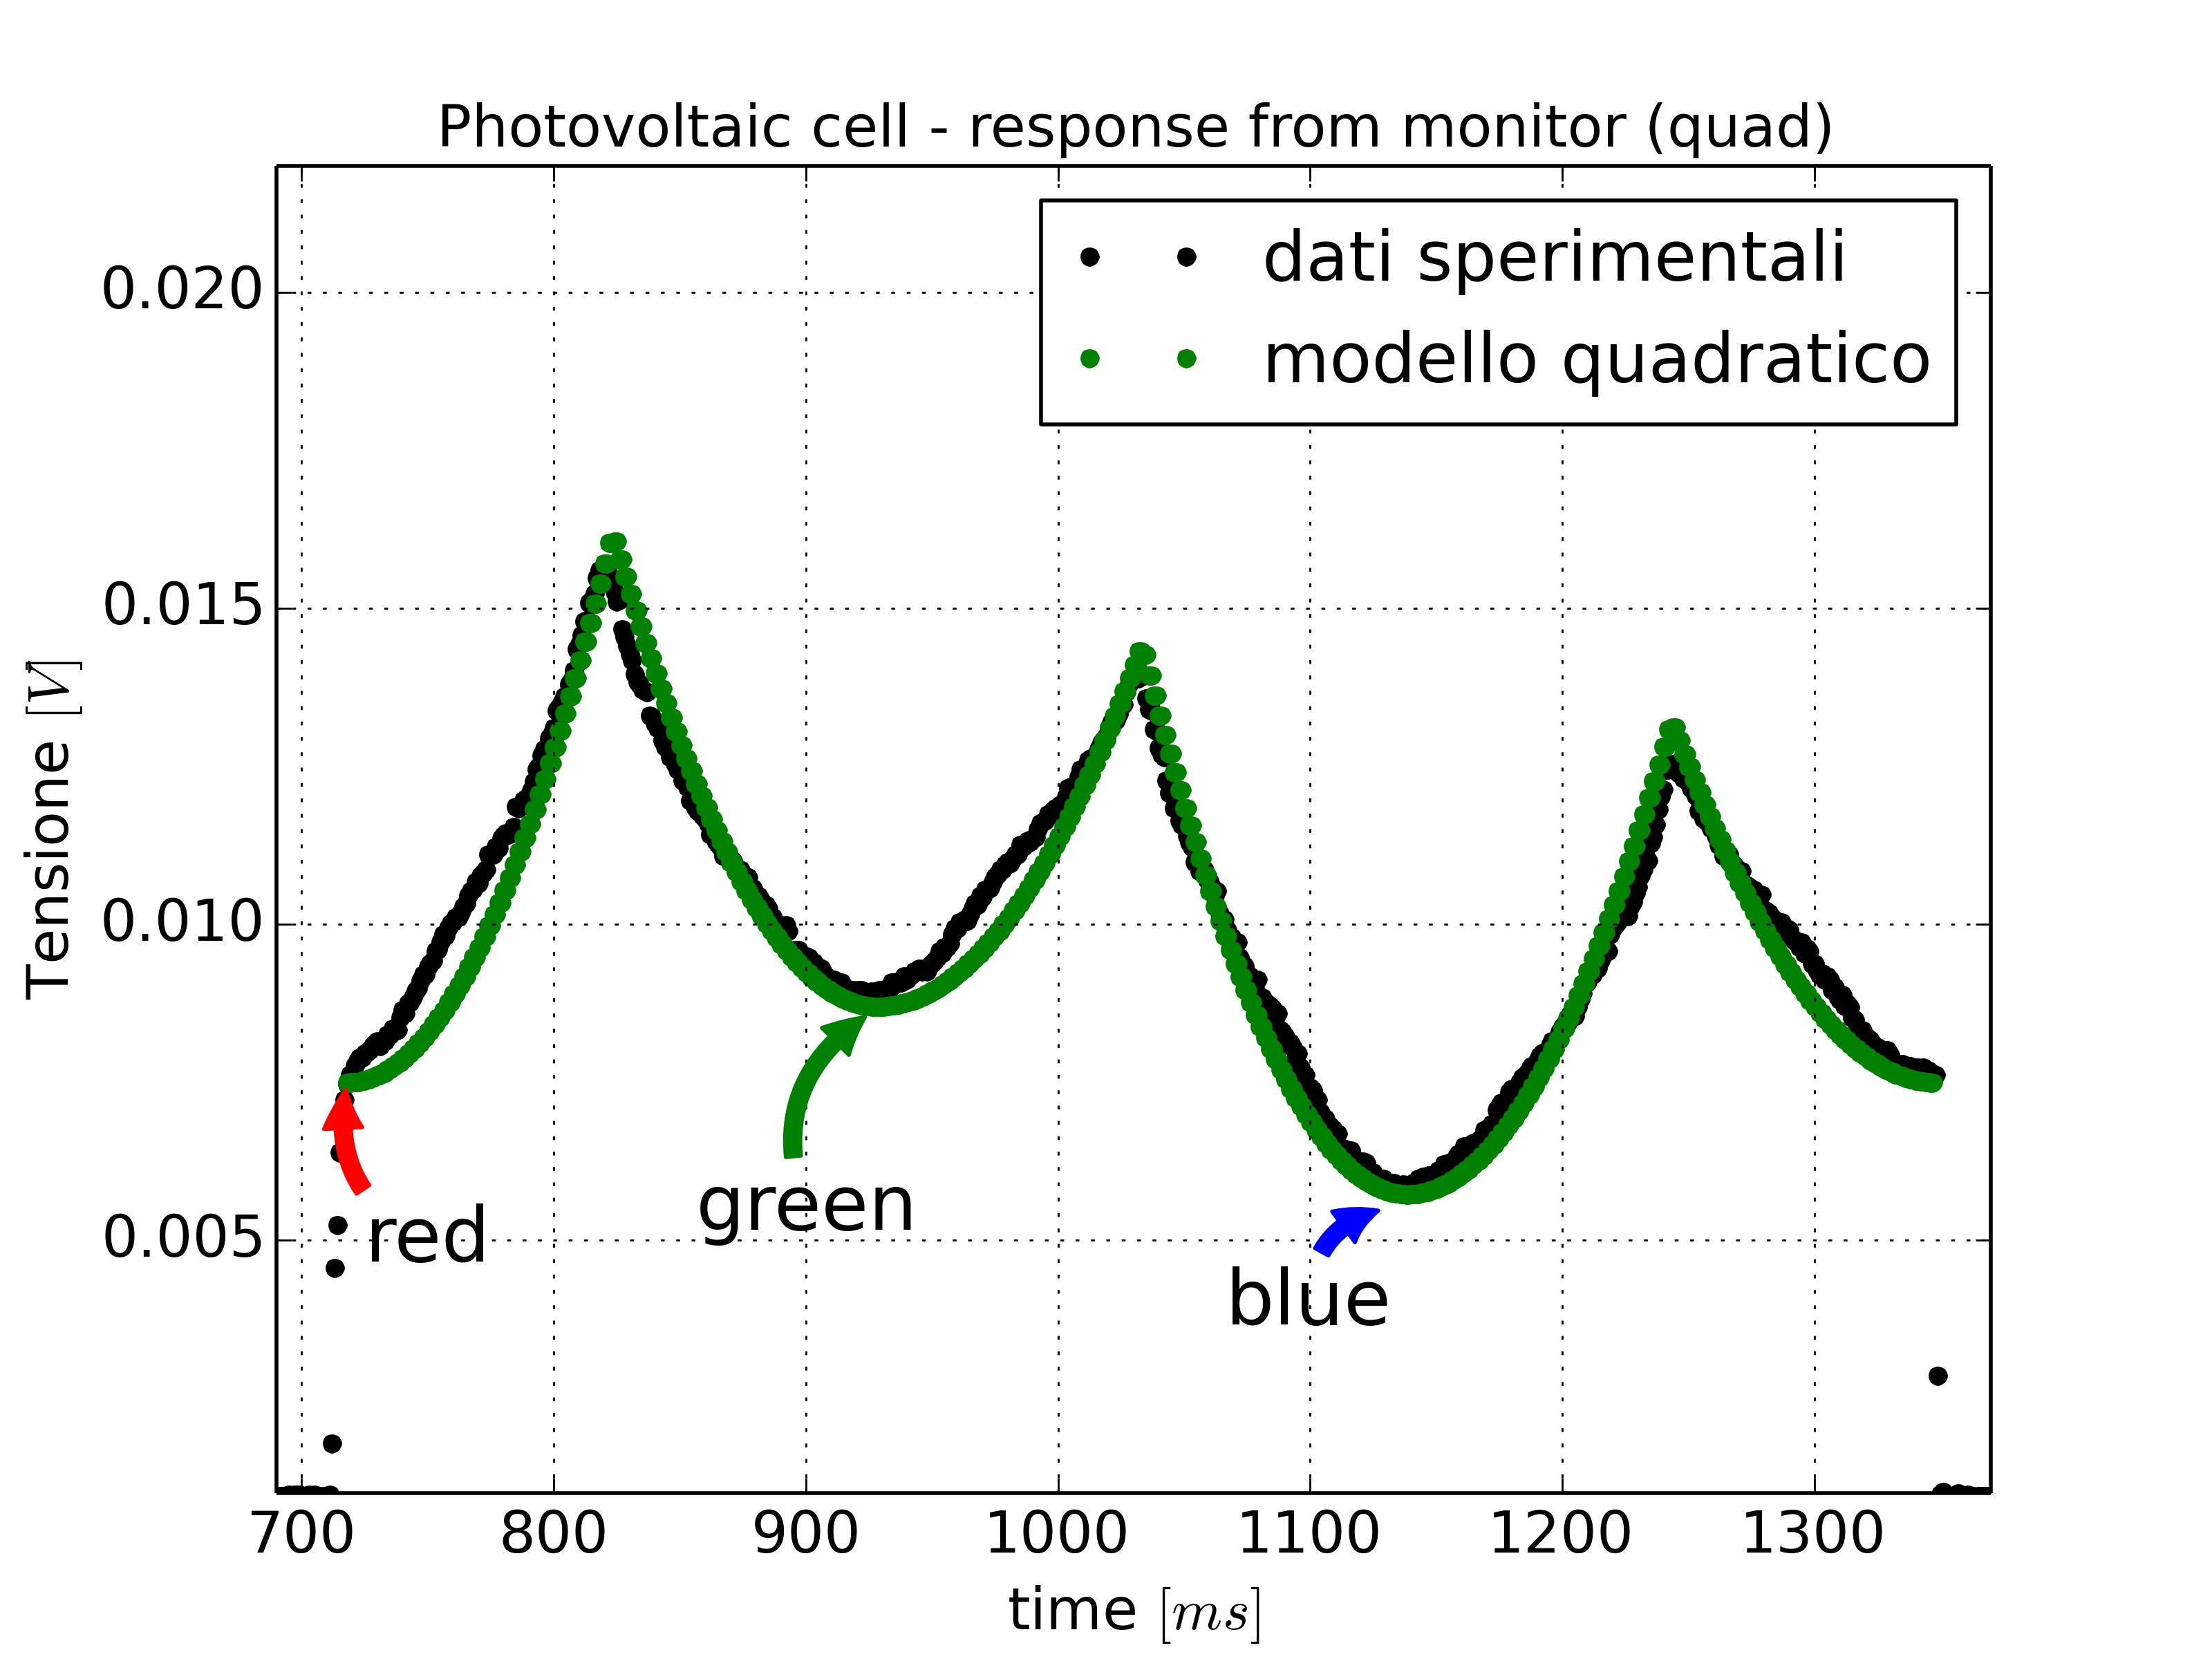
\includegraphics[width=0.6\linewidth]{./dati_quad}
\label{fig:dati_quad}}
%\qquad
\subfloat[Subfigure 2 list of figures text][Curva normalizzata del modello quadratico]{
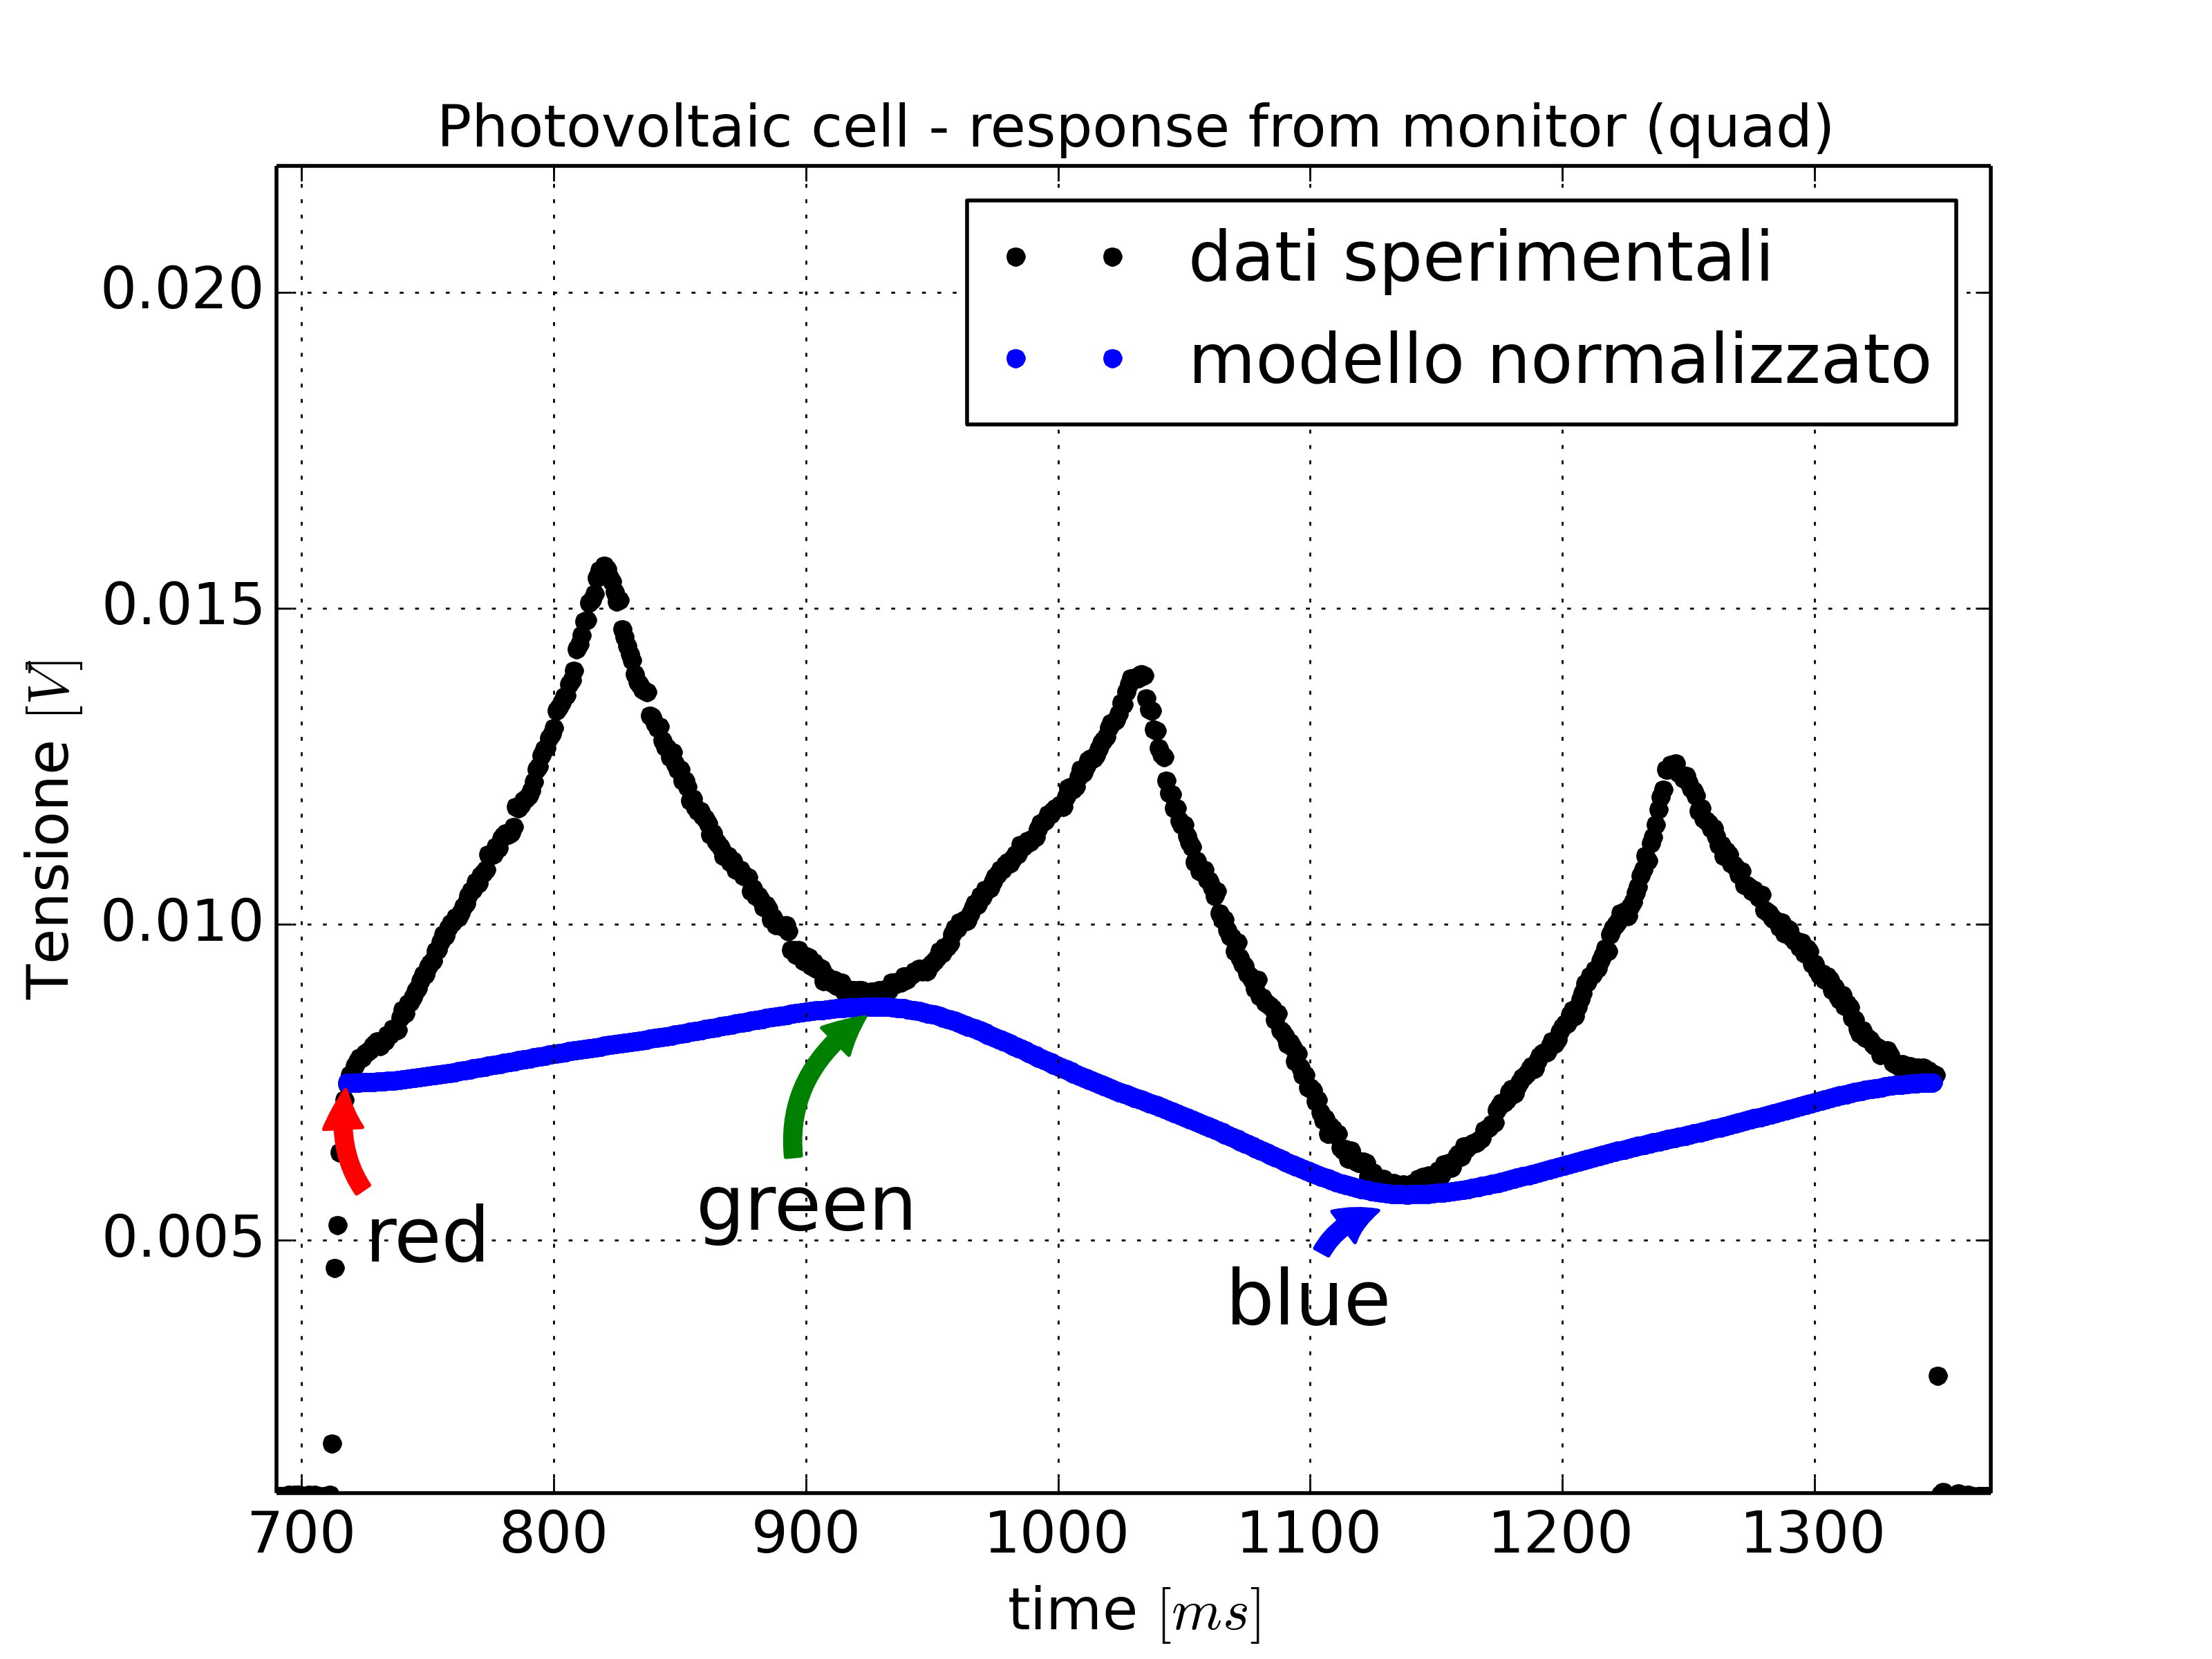
\includegraphics[width=0.6\linewidth]{./dati_normal}
\label{fig:dati_norm}}
%\qquad

\caption{}
\label{modello_quad}
\end{figure}


\item Idealmente, se il nostro monitor fosse stato composto da un numero piuttosto grande di LED ciascuno con la propria lunghezza d'onda e capaci di visualizzare (molti) var\^{\i} colori, si sarebbero potute identificare con il sensore analogico le $\lambda$ per tracciare la curva di responsività della fotocellula al silicio, ottenendo un importante risultato del punto di vista fisico. Tuttavia, come abbiamo ampiamente già detto, proprio a causa del principio di funzionamento di un monitor a LCD questo non è possibile. 

\end{itemize} 

Mettiamo da parte per il momento queste importanti precisazioni per affrontare in modo più generale il problema della riproduzione dei colori sullo schermo e della loro visualizzazione.\\
Introduciamo il concetto di \textbf{gamut} dei colori, strettamente legato alla creazione di un set di coordinate opportuno in cui questi possono essere rappresentati. Definito un set adeguato, infatti, il gamut è essenzialmente quella porzione di spazio che racchiude i colori che possono essere rappresentati da un dispositivo o rilevati (ad esempio dall'occhio umano). Esistono molti modelli di colore (tra cui l'RGB, il CMYK...) e modi differenti per definire le coordinate per ciascuno di questi. Un sistema standard è il \textsc{CIE 1931 XYZ colour space} creato dalla Commision Internationalle d'Eclaraige (CIE) nel 1931. Questo modello deriva da alcuni esperimenti portati avanti da Wright e Guild  negli anni '20 del secolo scorso che miravano a legare in qualche modo le proprietà fisiche di un colore (la lunghezza d'onda) con la percezione fisiologica di quest'ultimo da parte dell'occhio umano. I loro risultati sono stati integrati nelle specifiche del CIE RGB e le coordinate XYZ sono quelle usate più comunemente (anche nel gamut di Figura (\ref{fig:8_CIExy1931_sRGB_gamut_D65}). La definizione di quest'ultime si basa sull'introduzione delle cosiddette \textit{colour matching functions} $\bar{x}, \bar{y}, \bar{z}$, rappresentate in Figura (\ref{fig:446px-CIE_1931_XYZ_Color_Matching_Functions})): le matching functions sono definite dallo standard CIE in modo tale da riprodurre la responsività dei tre tipi di coni presenti nell'occhio. In particolare la $\bar{y}$ è detta \textit{luminosity function}: essendo centrata sul verde descrive la sensitività spettrale media della percezione visuale della luminosità da parte dell'occhio umano. Notiamo, \textit{en passant}, che queste curve non sono del tutto assimilabili a dei picchi centrati attorno alla rispettiva lunghezza d'onda, in quanto sono pesate in maniera diversa e forma differente.\\
Tramite le colour matching functions, definiamo ora in maniera precisa le coordinate XYZ già presentate:

\begin{equation}
\mathrm{X} = \int_{380}^{780} M(\lambda) \bar{x}(\lambda) \mathrm{d} \lambda
\end{equation}

\begin{equation}
\mathrm{Y} = \int_{380}^{780} M(\lambda) \bar{y}(\lambda) \mathrm{d} \lambda
\end{equation}

\begin{equation}
\mathrm{Z} = \int_{380}^{780} M(\lambda) \bar{z}(\lambda) \mathrm{d} \lambda
\end{equation}

Dove $M(\lambda)$ è lo spettro in lunghezza d'onda della radiazione incidente sul rivelatore.\\
Le coordinate XYZ sono anche dette "funzioni di tri-stimolo" (\textit{tristimulus functions}). Qualitativamente, i valori di tristimolo per un determinato spazio dei colori possono essere concettualizzate come la percentuale dei colori primari in un modello additivo tri-cromatico come è appunto l'RGB. In riferimento a quanto già detto, questi colori "primari" impiegati nella definizione non corrispondono a colori reali, cioè non sono generati da nessuna lunghezza d'onda definita. Le coordinate del gamut in Figura () sono proprio le funzioni di tristimolo Y e X (eventualmente normalizzate).\\

\begin{figure}
\centering
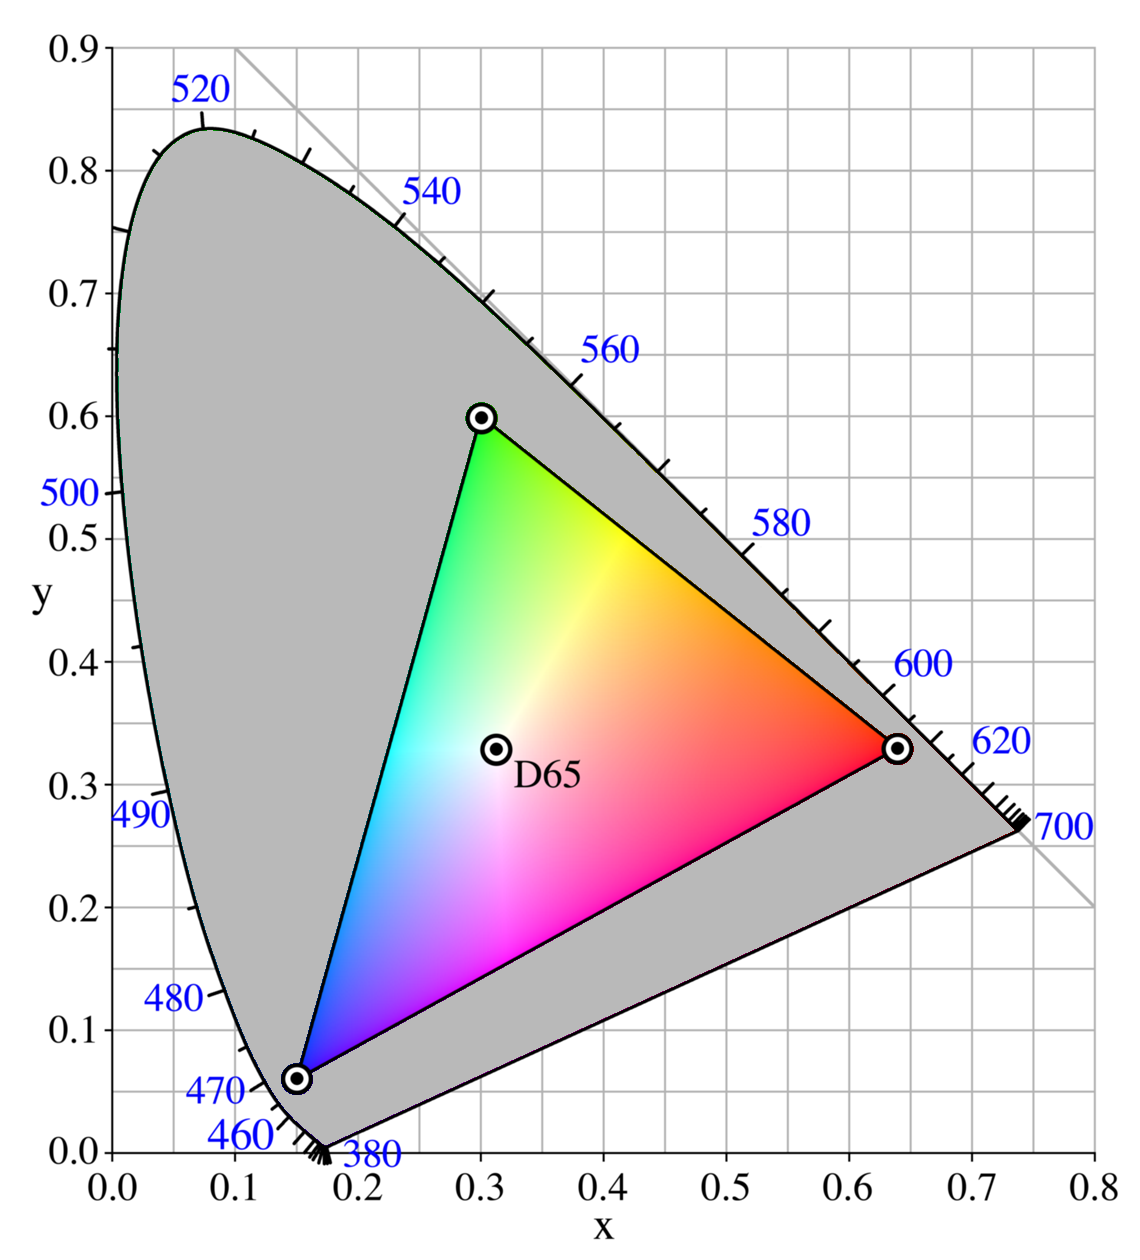
\includegraphics[width=0.7\linewidth]{./8_CIExy1931_sRGB_gamut_D65}
\caption{gamut dei colori su schermo RGB}
\label{fig:8_CIExy1931_sRGB_gamut_D65}
\end{figure}



\begin{figure}
\centering
\includegraphics[width=0.7\linewidth]{./446px-CIE_1931_XYZ_Color_Matching_Functions}
\caption{Color matching functions.}
\label{fig:446px-CIE_1931_XYZ_Color_Matching_Functions}
\end{figure}


%The tristimulus values associated with a colour space can be conceptualized as amounts of three primary colours in a tri-chromatic additive colour model. In some colour spaces, including LMS and XYZ spaces, the primary colours used are not real colours, in the sense that they cannot be generated with any light spectrum.
Dopo questa breve dissertazione, torniamo ora ai dati dell'intensità normalizzata rilevata dalla fotocellula. Durante quest'ultima esperienza, tramite l'uso del sensore \textsc{WS-7.56-TO5}, è stato possibile assegnare ad ogni tripletta RGB un valore di "pseudo" lunghezza d'onda (il cui significato è quello usuale di $\lambda$ della radiazione corrispondente ai colori puri R,G,B), cosa che non è stata possibile durante la week09. Proviamo a plottare quindi i dati dell'intensità luminosa normalizzata con il modello quadratico ormai ben noto, in funzione della "pseudo" lunghezza d'onda assegnata ad ogni tripletta RGB. Il grafico è in Figura (\ref{fig:nostro_gamut}).
Il risultato è davvero interessante: in particolare è facile notare la fortissima somiglianza con un tipico gamut dei colori riproducibili su un monitor LCD. Vogliamo cercare di capire se vi è qualche equivalenza fra gli assi da noi usati per il plot (luminosità-"pseudo"$\lambda$) e i valori di tristimolo (Y-X) dello spazio CIE:

\begin{figure}
\centering
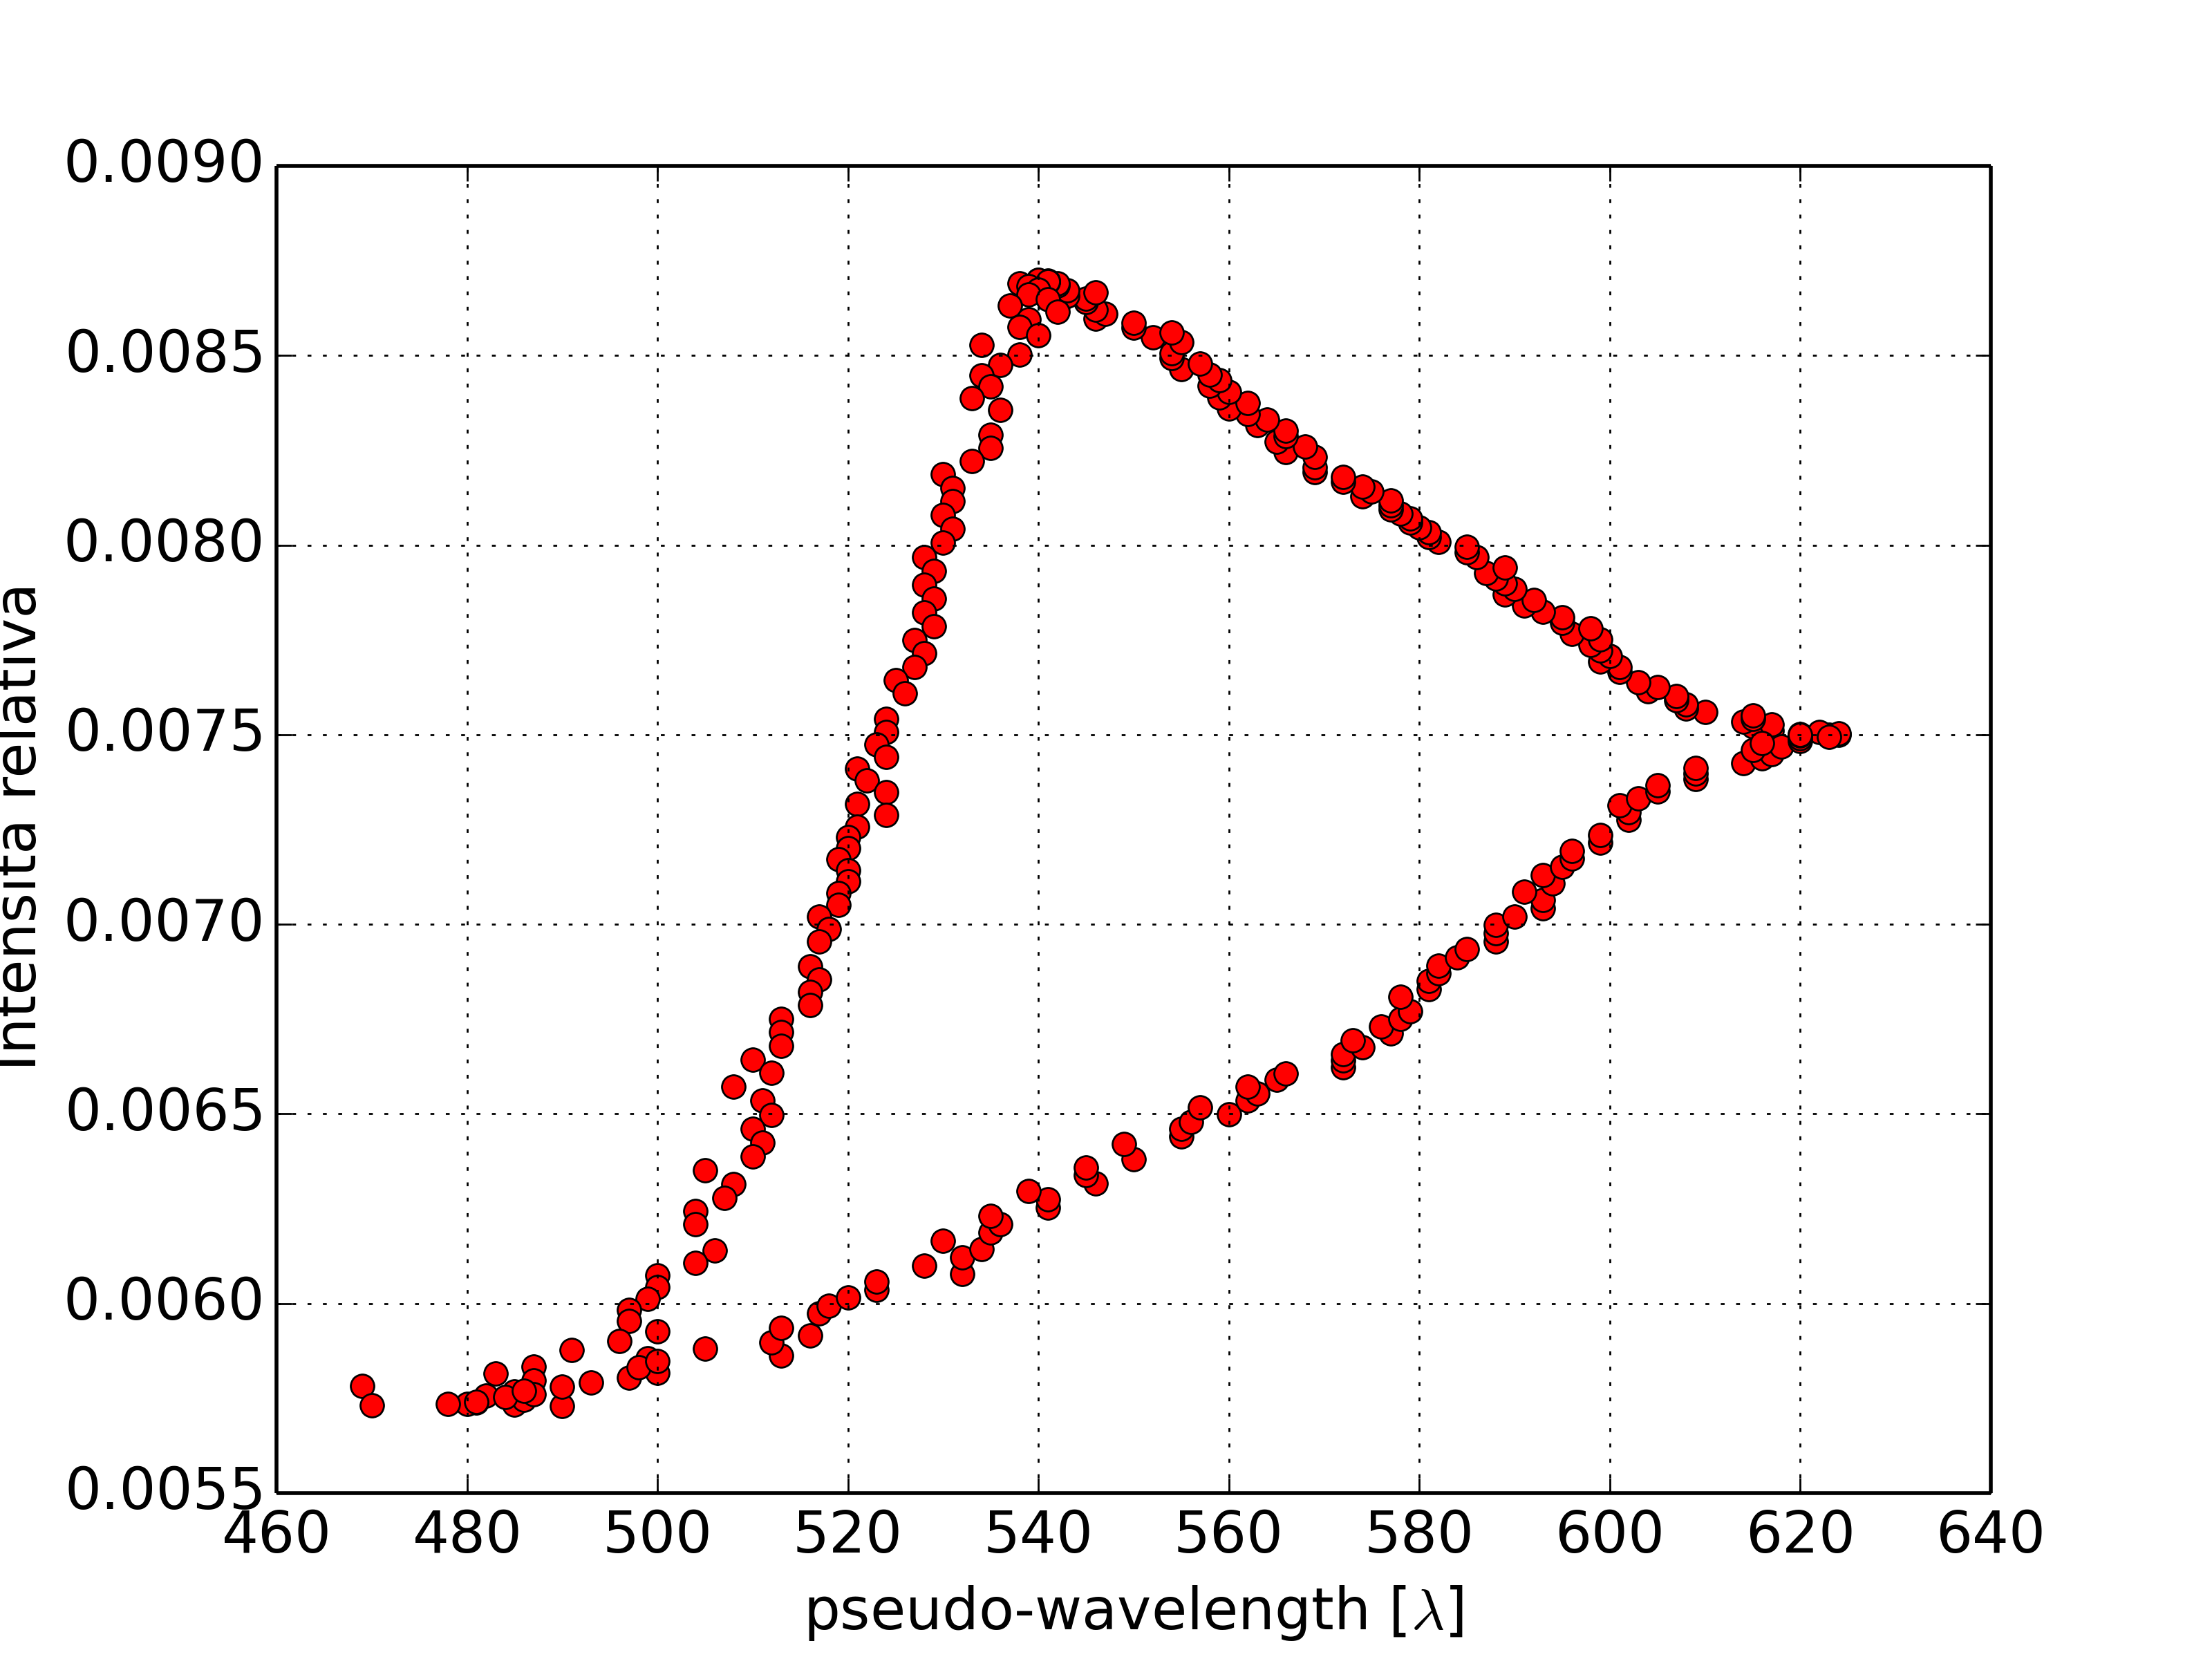
\includegraphics[width=0.7\linewidth]{./nostro_gamut}
\caption{Grafico della luminosità relativa in funzione della "pseudo" lunghezza d'onda}
\label{fig:nostro_gamut}
\end{figure}


\begin{itemize}
\item Si è già detto che il valore di tristimolo Y è definito in base alla luminosity function $\bar{y}(\lambda)$ che produce quindi una misura della luminosità della radiazione incidente come questa è percepita dall'occhio umano a causa del diverso bilanciamento delle tre tipologie di coni presenti (in particolare una maggiore presenza di colore verde porta ad una luminosità rilevata più alta). Più precisamente, la fotocellula stessa ha una curva di responsività che approssima quella dell'occhio, per questo motivo è possibile identificare in maniera abbastanza immediata il nostro asse delle ordinate con quello dello spazio dei colori CIE1931.

\item Per quanto riguarda l'asse delle ascisse il discorso è un po' più delicato. Il valore di tristimolo X effettivamente è legato in prima approssimazione alla quantità di colore rosso presente nella radiazione incidente e classifica quest'ultima da un minimo ad un massimo, dove il minimo corrisponde al blu (il picco del blu è il più lontano dalla color matching fuunction $\bar{x}$ e quindi l'integrale su quest'ultima dà il valore più basso) e il massimo corrisponde al rosso stesso: l'integrazione restituisce valore massimo poichè le due curve sono praticamente sovrapposte. Non è banale capire qual è il processo per cui, a partire da una radiazione composta da un miscuglio di lunghezze d'onda differenti, tramite il sensore analogico si può estrarre una "lunghezza d'onda" risultante: questo valore non è semplicemente quello della radiazione prevalente, come dimostra l'esempio riportato in precedenza delle triplette (0.4,1,0), (0.8,0,1) per cui viene rilevata una "pseudo" $\lambda$ di circa 550nm, date anche le proporzioni confrontabili delle intensità dei due LED per cui non ve n'è una molto più piccola dell'altra. Ad ogni modo, fenomenologicamente possiamo osservare che l'aspetto che conta davvero è che i diversi colori prodotti dal monitor vengono classificati in maniera \underline{analoga} a quanto verrebbe fatto con l'integrale sulla funzione matching: da sinistra verso destra si procede andando dal blu al rosso e questa "pseudo" lunghezza d'onda è tanto maggiore quanto più ci si avvicina al colore rosso (a livello dei colori puri quest'ultima osservazione è ovvia). Per questi motivi, nonostante risulti azzardato identificare un'equivalenza fra le due scale X e $\lambda$, l'ordinamento dei colori è analogo per entrambe e possiamo quindi affermare di aver misurato il gamut del nostro monitor LCD.
\end{itemize}

\begin{thebibliography}{10}

\bibitem{bib3}
Thomas J. Bruno, Paris D. N. Svoronos. CRC Handbook of Fundamental Spectroscopic Correlation Charts

\end{thebibliography}



\end{document}